% -*- Mode:TeX -*-

%% IMPORTANT: The official thesis specifications are available at:
%%            http://libraries.mit.edu/archives/thesis-specs/
%%
%%            Please verify your thesis' formatting and copyright
%%            assignment before submission.  If you notice any
%%            discrepancies between these templates and the 
%%            MIT Libraries' specs, please let us know
%%            by e-mailing thesis@mit.edu

%% The documentclass options along with the pagestyle can be used to generate
%% a technical report, a draft copy, or a regular thesis.  You may need to
%% re-specify the pagestyle after you \include  cover.tex.  For more
%% information, see the first few lines of mitthesis.cls. 

%\documentclass[12pt,vi,twoside]{mitthesis}
%%
%%  If you want your thesis copyright to you instead of MIT, use the
%%  ``vi'' option, as above.
%%
%\documentclass[12pt,twoside,leftblank]{mitthesis}
%%
%% If you want blank pages before new chapters to be labelled ``This
%% Page Intentionally Left Blank'', use the ``leftblank'' option, as
%% above. 

\documentclass[12pt,twoside]{mitthesis}
\usepackage{lgrind}
%% These have been added at the request of the MIT Libraries, because
%% some PDF conversions mess up the ligatures.  -LB, 1/22/2014
\usepackage{cmap}
\usepackage[english]{babel}
\usepackage[utf8]{inputenc}
\usepackage{algorithm,algpseudocode,amsmath,amssymb,amsfonts,amsthm,array,bm,caption,cases,color,fancybox,fancyhdr,float,fontenc,geometry,graphicx,lipsum,pdfpages,subcaption,tikz,times,thmbox,xcolor}
\pagestyle{plain}

%% This bit allows you to either specify only the files which you wish to
%% process, or `all' to process all files which you \include.
%% Krishna Sethuraman (1990).
\makeatletter
\renewcommand*\env@matrix[1][\arraystretch]{%
  \edef\arraystretch{#1}%
  \hskip -\arraycolsep
  \let\@ifnextchar\new@ifnextchar
  \array{*\c@MaxMatrixCols c}}
\makeatother


\begin{document}

% -*-latex-*-
% 
% For questions, comments, concerns or complaints:
% thesis@mit.edu
% 
%
% $Log: cover.tex,v $
% Revision 1.8  2008/05/13 15:02:15  jdreed
% Degree month is June, not May.  Added note about prevdegrees.
% Arthur Smith's title updated
%
% Revision 1.7  2001/02/08 18:53:16  boojum
% changed some \newpages to \cleardoublepages
%
% Revision 1.6  1999/10/21 14:49:31  boojum
% changed comment referring to documentstyle
%
% Revision 1.5  1999/10/21 14:39:04  boojum
% *** empty log message ***
%
% Revision 1.4  1997/04/18  17:54:10  othomas
% added page numbers on abstract and cover, and made 1 abstract
% page the default rather than 2.  (anne hunter tells me this
% is the new institute standard.)
%
% Revision 1.4  1997/04/18  17:54:10  othomas
% added page numbers on abstract and cover, and made 1 abstract
% page the default rather than 2.  (anne hunter tells me this
% is the new institute standard.)
%
% Revision 1.3  93/05/17  17:06:29  starflt
% Added acknowledgements section (suggested by tompalka)
% 
% Revision 1.2  92/04/22  13:13:13  epeisach
% Fixes for 1991 course 6 requirements
% Phrase "and to grant others the right to do so" has been added to 
% permission clause
% Second copy of abstract is not counted as separate pages so numbering works
% out
% 
% Revision 1.1  92/04/22  13:08:20  epeisach

% NOTE:
% These templates make an effort to conform to the MIT Thesis specifications,
% however the specifications can change.  We recommend that you verify the
% layout of your title page with your thesis advisor and/or the MIT 
% Libraries before printing your final copy.
\title{Calibration and Fusion of Stereoscopic Cameras and Optical Range Finder Sensors for Zero Gravity Targets Inspection}

\author{Gabriel P. Urbain}
% If you wish to list your previous degrees on the cover page, use the 
% previous degrees command:
%       \prevdegrees{A.A., Harvard University (1985)}
% You can use the \\ command to list multiple previous degrees
%       \prevdegrees{B.S., University of California (1978) \\
%                    S.M., Massachusetts Institute of Technology (1981)}
\department{Department of Electronics, Optronics and Signal Processing (DEOS)}

% If the thesis is for two degrees simultaneously, list them both
% separated by \and like this:
% \degree{Doctor of Philosophy \and Master of Science}
\degree{Master of Science in Aerospace Engineering}

% As of the 2007-08 academic year, valid degree months are September, 
% February, or June.  The default is June.
\degreemonth{October}
\degreeyear{2014}
\thesisdate{October 23, 2014}

%% By default, the thesis will be copyrighted to MIT.  If you need to copyright
%% the thesis to yourself, just specify the `vi' documentclass option.  If for
%% some reason you want to exactly specify the copyright notice text, you can
%% use the \copyrightnoticetext command.  
%\copyrightnoticetext{\copyright IBM, 1990.  Do not open till Xmas.}

% If there is more than one supervisor, use the \supervisor command
% once for each.
\supervisor{Alvar Saenz-Otero}{Principal Research Scientist, Space Systems Laboratory, MIT}
\supervisor{Daniel Alazard}{Professor, Department of Mathematics, Computer Science and Control (DMIA), ISAE Supaero}

% This is the department committee chairman, not the thesis committee
% chairman.  You should replace this with your Department's Committee
% Chairman.
\chairman{moi}{moi}
% Make the titlepage based on the above information.  If you need
% something special and can't use the standard form, you can specify
% the exact text of the titlepage yourself.  Put it in a titlepage
% environment and leave blank lines where you want vertical space.
% The spaces will be adjusted to fill the entire page.  The dotted
% lines for the signatures are made with the \signature command.
\maketitle

% The abstractpage environment sets up everything on the page except
% the text itself.  The title and other header material are put at the
% top of the page, and the supervisors are listed at the bottom.  A
% new page is begun both before and after.  Of course, an abstract may
% be more than one page itself.  If you need more control over the
% format of the page, you can use the abstract environment, which puts
% the word "Abstract" at the beginning and single spaces its text.

%% You can either \input (*not* \include) your abstract file, or you can put
%% the text of the abstract directly between the \begin{abstractpage} and
%% \end{abstractpage} commands.

% First copy: start a new page, and save the page number.
\cleardoublepage
% Uncomment the next line if you do NOT want a page number on your
% abstract and acknowledgments pages.
% \pagestyle{empty}
\setcounter{savepage}{\thepage}
\begin{abstractpage}
In many areas of robotics, vision is becoming more and more common in applications such as localization, automatic map construction, autonomous navigation, path following, inspection, monitoring or risky situation detection. With the increasing performances of embedded computers and the development of faster algorithms in the last few years, multi-sensors data fusion is considered as an opportunity to take better advantage of different sensors characteristics and stretch the limits. This project aims at implementing a multi-sensor data fusion algorithm involving two stereoscopic cameras of and a Time-of-Flight camera (TOF) on in-space nano-satellites called SPHERES.\\
This document is the result of five months internship at the MIT SSL, USA as part of the final project of a double Master degree in Aerospace Engineering at ISAE, France and Electrical Engineering at UMONS, Belgium. The first chapter introduces the goal and the context of the project. The second chapter is dedicated to the theoretical aspect and aims at summarizing the required mathematical background and development. A third chapter analyzes concretely the implementation and finally, the results of two different experiments set will be detailed in the fourth chapter before to conclude.
\end{abstractpage}

% Additional copy: start a new page, and reset the page number.  This way,
% the second copy of the abstract is not counted as separate pages.
% Uncomment the next 6 lines if you need two copies of the abstract
% page.
% \setcounter{page}{\thesavepage}
% \begin{abstractpage}
% % $Log: abstract.tex,v $
% Revision 1.1  93/05/14  14:56:25  starflt
% Initial revision
% 
% Revision 1.1  90/05/04  10:41:01  lwvanels
% Initial revision
% 
%
%% The text of your abstract and nothing else (other than comments) goes here.
%% It will be single-spaced and the rest of the text that is supposed to go on
%% the abstract page will be generated by the abstractpage environment.  This
%% file should be \input (not \include 'd) from cover.tex.
In this thesis, I designed and implemented a compiler which performs
optimizations that reduce the number of low-level floating point operations
necessary for a specific task; this involves the optimization of chains of
floating point operations as well as the implementation of a ``fixed'' point
data type that allows some floating point operations to simulated with integer
arithmetic.  The source language of the compiler is a subset of C, and the
destination language is assembly language for a micro-floating point CPU.  An
instruction-level simulator of the CPU was written to allow testing of the
code.  A series of test pieces of codes was compiled, both with and without
optimization, to determine how effective these optimizations were.

% \end{abstractpage}

\cleardoublepage

\section*{Acknowledgments}
I am grateful to all the great people who helped me throughout this internship, starting with Alvar Saenz-Otero, who welcomed me in his lab and always took the time to guide me, all SSL staff for their help and their advice, Daniel Alazard who accelerated the administrative process, Marina G. March who undertake this experience on my side as well as all my professors in Mons and Toulouse and especially Ir. S. Lizy-Destrez and Pr. T. Dutoit who helped me personally in all my projects.\\\\
I also would like to thank GDF Suez, the University of Mons and the Fernand Lazard Foundation for the financial support they provided during this internship.\\\\
Finally, I give the biggest thanks of all to my parents, my sister and my friends in Mons and Supaero who, through their support, their energy and their smile, made my six years at university the most unforgettable experience ever.

%%%%%%%%%%%%%%%%%%%%%%%%%%%%%%%%%%%%%%%%%%%%%%%%%%%%%%%%%%%%%%%%%%%%%%
% -*-latex-*-

% Some departments (e.g. 5) require an additional signature page.  See
% signature.tex for more information and uncomment the following line if
% applicable.
% % -*- Mode:TeX -*-
%
% Some departments (e.g. Chemistry) require an additional cover page
% with signatures of the thesis committee.  Please check with your
% thesis advisor or other appropriate person to determine if such a 
% page is required for your thesis.  
%
% If you choose not to use the "titlepage" environment, a \newpage
% commands, and several \vspace{\fill} commands may be necessary to
% achieve the required spacing.  The \signature command is defined in
% the "mitthesis" class
%
% The following sample appears courtesy of Ben Kaduk <kaduk@mit.edu> and
% was used in his June 2012 doctoral thesis in Chemistry. 

\begin{titlepage}
\begin{large}
%This doctoral thesis has been examined by a Committee of the Department
%of Chemistry as follows:

%\signature{Professor Jianshu Cao}{Chairman, Thesis Committee \\
%   Professor of Chemistry}

%\signature{Professor Troy Van Voorhis}{Thesis Supervisor \\
%   Associate Professor of Chemistry}

%\signature{Professor Robert W. Field}{Member, Thesis Committee \\
%   Haslam and Dewey Professor of Chemistry}
\end{large}
\end{titlepage}


\pagestyle{plain}
  % -*- Mode:TeX -*-
%% This file simply contains the commands that actually generate the table of
%% contents and lists of figures and tables.  You can omit any or all of
%% these files by simply taking out the appropriate command.  For more
%% information on these files, see appendix C.3.3 of the LaTeX manual. 
\tableofcontents
\newpage
\listoffigures
\newglossaryentry{FOV}{name=FOV, description={Field-of-View}}
\newglossaryentry{ORF}{name=ORF, description={Optical Range Finder}}
\newglossaryentry{ToF}{name=ToF, description={Time-of-Flight}}

\newglossaryentry{SPHERES}{name=SPHERES, description={Synchronized Position Hold, Engage, Reorient Experimental Satellites}}
\newglossaryentry{VERTIGO}{name=VERTIGO, description={Visual Estimation for Relative Tracking and Inspection of Generic Objects}}
\newglossaryentry{INSPECT}{name=INSPECT, description={Integrated Navigation Sensor Platform for EVA Control and Testing}}
\newglossaryentry{EVA}{name=EVA, description={Extra Vehicular Activity}}
\newglossaryentry{MIT}{name=MIT, description={Massachusetts Institute of Technology}}
\newglossaryentry{ISAE}{name=ISAE, description={Instititut Superieur de l'Aeronautique et de l'Espace}}
\newglossaryentry{SSL}{name=SSL, description={Space System Laboratory}}
\newglossaryentry{HEOMD}{name=HEOMD, description={NASA Human Exploration and Operations Mission Directorate}}
\newglossaryentry{CMG}{name=CMG, description={Control Moment Gyroscope}}
\newglossaryentry{RGA}{name=RGA, description={Reduced Gravity Aircraft}}
\newglossaryentry{DoF}{name=DoF, description={Degree of Freedom}}
\newglossaryentry{ISS}{name=ISS, description={International Space Station}}
\printglossaries


% % First Chapter : Introduction
%
% Master Thesis: Calibration and fusion of stereo cameras and optical-range finder sensors
% for in-space localization and mapping
%
% Achieved at Space System Lab, M.I.T.
% Supervisor: Alvar Saenz-Otero, Daniel Alazard
%
% Institut Sup�rieur de l'A�ronautique et de l'Espace
% Major: Telecommunications et r�seaux - Syst�mes Spatiaux et Lanceurs
% Gabriel Urbain - October 2014
%%

\chapter{Introduction}

\section{Context}
\subsection{SPHERES}
\subsection{HALO}
\subsection{INSPECT}

\section{Objectives}
3 Sensors. Architecture. 2 sections: calibration and fusion.



% % Second Chapter : Theoritical Approach
%
% Master Thesis: Calibration and Fusion of Stereoscopic and Time-of-Flight 
% Cameras for Zero Gravity Targets Inspection
%
% Achieved at Space System Lab, M.I.T.
% Supervisor: Alvar Saenz-Otero, Daniel Alazard
%
% Institut Sup�rieur de l'A�ronautique et de l'Espace
% Major: Telecommunications et r�seaux - Syst�mes Spatiaux et Lanceurs
% Gabriel Urbain - October 2014
%%

\chapter{Theoretical Approach}
\label{chapter:theory}

In this chapter, we will try to give all the theoretical tools to understand the algorithm development carried out in this project. The first section aims at reminding the reader of background models and theories but we will assume he masters his basics of mechanics of the rigid body, optics, image processing, numerical analysis and computer sciences.
Section two focuses on calibration algorithm. It reviews solutions found in the literature to calibrate separately stereoscopic cameras and a \gls{ToF} camera but also describes the implementation and adaptation of a new algorithm proposed in \cite{stereo_tof_fusion_proba} to calibrate the whole \gls{ToF} and stereo cameras system while taking advantage of each sensors characteristics.
Finally, the last section analyzes the core implementation of the fusion algorithm tested in this project, try to set out arguments to the choices that have been made and describes each parts in details.

\section{Camera Model Elaboration}
Before going into further details into the algorithms breakdown, it may be necessary to clarify the models employed throughout this document. Indeed, to simplify the sensor fusion analysis and implementation, we will have to make numerous simplifications and hypothesis about the camera models that we shall remember in Chapter 4 where experimental results are discussed.

\subsection{Mathematical Notations}
Several coordinates systems are used in this work leading themselves to many different transformations between each others. To give the reader a better overview, this paragraph summarizes the mathematical notations employed in this document.

\paragraph{Coordinates Systems:}
\begin{itemize*}
\item $\mathbf{T}$: Coordinate system of the \gls{ToF}) camera (or \gls{ORF}). In the 3D system, the origin is situated in the pinhole, the  $Z$ axis points forward, $Y$ axis points down and $X$ points right. In the 2D coordinate system, the origin is situated in the top left corner of the image plane,$U$ points to the right and $V$ points down.
\item $\mathbf{R}$: 3D coordinate system of the right camera of the stereo rig. In the 3D system, the origin is situated in the pinhole, the  $Z$ axis points forward, $Y$ axis points down and $X$ points right. In the 2D coordinate system, the origin is situated in the top left corner of the image plane,$U$ points to the right and $V$ points down.
\item $\mathbf{L}$: 3D coordinate system of the left camera of the stereo rig. In the 3D system, the origin is situated in the pinhole, the  $Z$ axis points forward, $Y$ axis points down and $X$ points right. In the 2D coordinate system, the origin is situated in the top left corner of the image plane,$U$ points to the right and $V$ points down.
\end{itemize*}

\paragraph{Transformations Matrices:}
To represent both affine (translation and rotation) and projective transformation  from one coordinate system to another, we use $4x4$ transformation matrices. For instance, in the case of an affine transformation of a point $P$ from $R$ to $L$ coordinate system, we write:
\begin{equation}
\begin{pmatrix}[0.8]
x_L\\
y_L\\
z_L\\
1
\end{pmatrix} = M_{LR} * \begin{pmatrix}[0.8]
x_R\\
y_R\\
z_R\\
1
\end{pmatrix}
\end{equation}
Where:
\begin{equation}
M_{LR} = \begin{pmatrix}[0.8]
r_{XX} & r_{XY} & r_{XZ} & t_X\\
r_{YX} & r_{YY} & r_{YZ} & t_Y\\
r_{ZX} & r_{ZY} & r_{ZZ} & t_Z
\end{pmatrix}
\end{equation}
Which allows to multiply matrices directly between each other:
\begin{equation}
M_{TR} = M_{TL} * M_{LR}
\end{equation}


\subsection{Pinhole Camera Model}
\label{sec:mono_camera}
According to \cite{epipolar_geometry}, a common representation of a camera is composed of a lens represented by a single pinhole $O$ in the \textit{focal plane }$\mathcal{F}$ and a sensor matrix in the \textit{image plane} $\mathcal{I}$ at a distance $f$ from the focal plane. As represented on figure \ref{fig:cam1}, $O$, also called optical center, is the origin of the world 3D coordinates system $OXYZ$ where $Z$ is perpendicular to the focal plane and directed in the opposite direction of the image plane and $X$ and $Y$ are included in the plane. The pixels on the image plane are localized with a 2D coordinates system $O'U'V'$ where the origin is situated in the lower-right corner of the sensor matrix. The $Z$ axis intersects $\mathcal{I}$ in a point $c' = (c_U', c_V')$ called the \textit{principal point}.

% Figure cam1
\begin{figure}[!htt]
	\begin{center}
		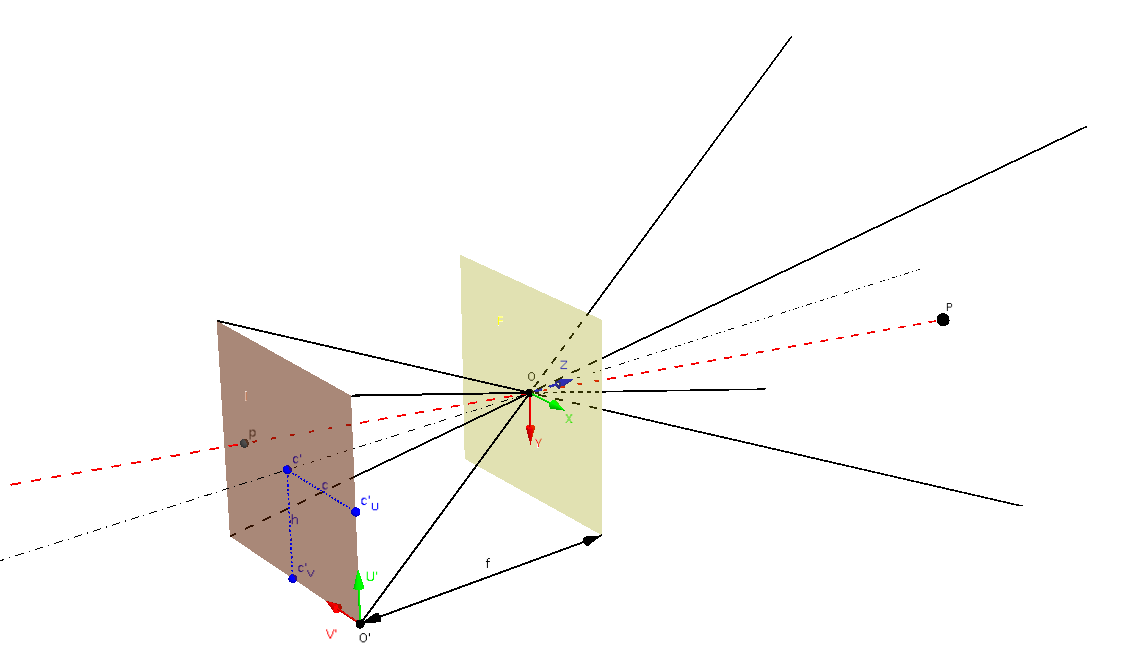
\includegraphics[width=15cm]{img/cam1.png}
		\caption{Geometry of the pinhole model for a single camera}
		\label{fig:cam1}
	\end{center}
\end{figure}

To facilitate the representation, we can consider a \textit{virtual image plane} at a distance $f$ on the positive $Z$ axis, which does not change anything to the problem but helps to recreate directly a \textit{projected image} with the same orientation than the real object. We now have a 2D coordinate system $O"UV$ (figure \ref{fig:cam2}).

% Figure cam2
\begin{figure}[!htt]
	\begin{center}
		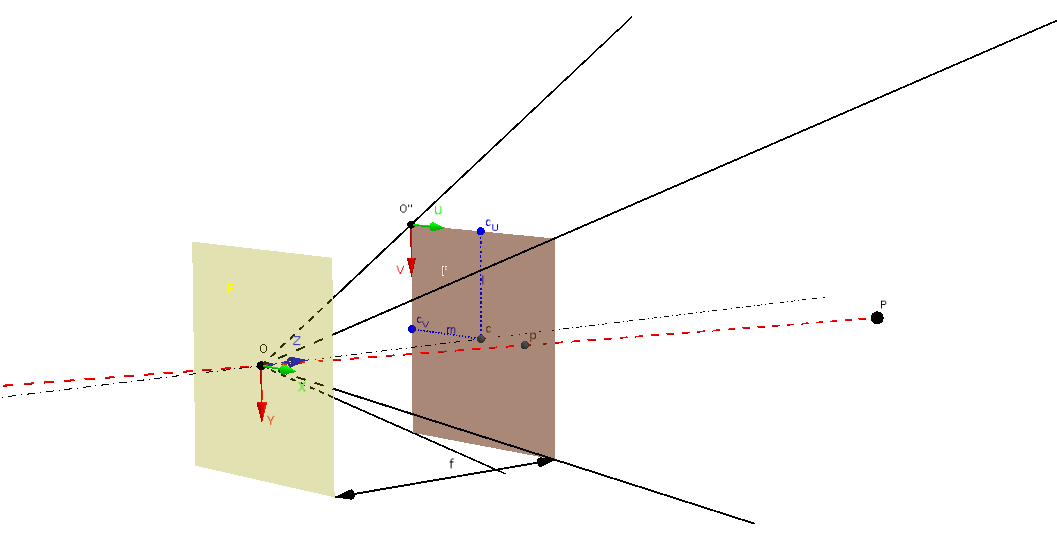
\includegraphics[width=15cm]{img/cam2.png}
		\caption{In this simplified representation, the point P is projected in the virtual plane}
		\label{fig:cam2}
	\end{center}
\end{figure}

In this optimal model, the \textit{intrinsic} geometry of the camera is completely represented by the parameters $f$, $c_U$ and $c_V$ measured in pixels. However, to make the model more realistic, we can introduce extra parameters such as:
\begin{itemize*}
\item The lens enlargement $k$, whose value is different along $u$ and $v$ axis and represented in the model by coordinates $f_U = k_U * f$ and $f_V = k_V * f$
\item The skew $s_{UV}$, assessing the non-orthogonality between rows and columns of the sensor photosensitive cells.
\end{itemize*}
Those five parameters $f_U$, $f_V$, $c_U$, $c_V$, $s_{UV}$ constitute what we call the \textit{intrinsic matrix} of the camera:
\begin{equation}
K =  \begin{pmatrix}
	f_U & s_{UV} & c_U\\
	0 & f_V & c_V\\
	0 & 0 & 1
	\end{pmatrix}
\end{equation}

Therefore, we can write the affine transformation linking a \textit{world point}, represented by its \textit{homogeneous coordinates} in the camera three-dimensional coordinates system and a \textit{projected point} represented by its \textit{homogeneous coordinates} in the image two-dimensional coordinates system:
\begin{equation}
\label{eq:pinhole}
s \begin{pmatrix}[0.8]
u\\
v\\
1
\end{pmatrix}
 = K * \begin{pmatrix}[0.8]
 x\\
 y\\
 z\\
 1
 	\end{pmatrix}
\end{equation}

Finally, the model can be refine to take the distortions into account. As proposed by Brown \cite{camera_distortion}, the distortion may be divided into radial and tangential and can be represented by a second degree polynomial which maps the undistorted and distorted images together thanks to 6 parameters. This will be detailed in section \ref{sec:calib}.\\

One should also notice that the parameters discussed here define the mathematical model of the camera but performances can be determined as well. For instance, the \textit{Field-Of-View} (\gls{FoV}) of the camera and the pixel size $\epsilon_p$ of the photosensitive cells (sometimes given by the pixel density, measured in pix/meters) are two characteristics to measure camera performances.

\subsection{Stereoscopic Cameras Model}
\label{sec:stereo_camera}
In the literature, the stereo camera is commonly represented as the assembly of two pinhole models whose focal points are separated by a distance called \textit{baseline}. As in figure \ref{fig:cam_stereo}, we thus have now two 3D coordinate systems $L = O_LX_LY_LZ_L$ and $R = O_RX_RY_RZ_R$.

% Figure cam_stereo
\begin{figure}[!htt]
	\begin{center}
		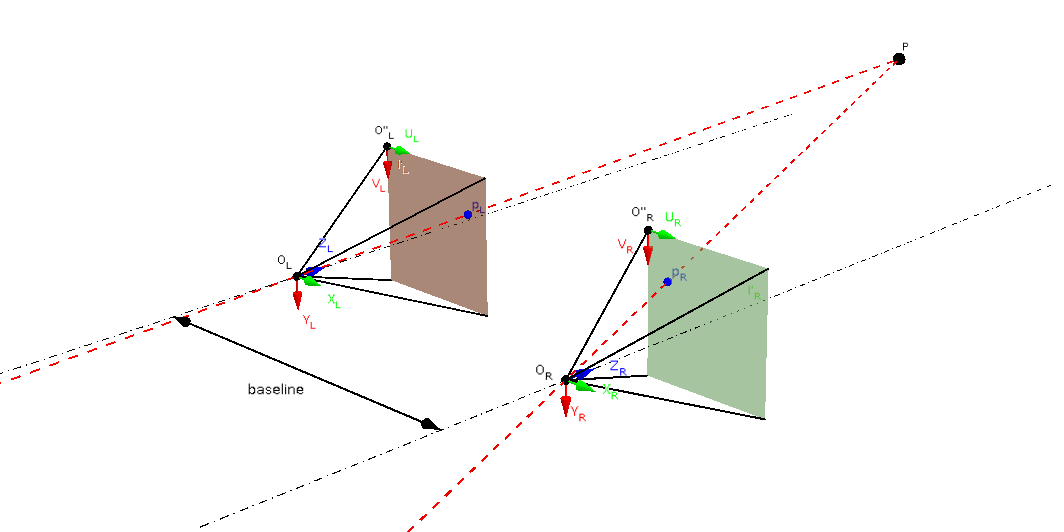
\includegraphics[width=15cm]{img/cam_stereo.png}
		\caption{Model of an assembly of stereoscopic cameras}
		\label{fig:cam_stereo}
	\end{center}
\end{figure}

\subsubsection{Projection}
We can still use the model developed in the precedent paragraph but the rotation and the translation between $L$ and $R$ must be taken into account when a point is represented in 3D. An \textit{extrincic matrix} is then defined to perform that transformation:
\begin{equation}
M =  \begin{pmatrix}
	r_{X,X'} & r_{X,Y'} & r_{X,Z'} & t_{X}\\
	r_{Y,X'} & r_{Y,Y'} & r_{Y,Z'} & t_{Y}\\
	r_{Z,X'} & r_{Z,Y'} & r_{Z,Z'} & t_{Z}
	\end{pmatrix}
\end{equation}

Which gives:
\begin{equation}
s \begin{pmatrix}
u\\
v\\
1
\end{pmatrix}
 = K * M * \begin{pmatrix}[0.8]
 x\\
 y\\
 z\\
 1
 	\end{pmatrix} = P * \begin{pmatrix}[0.8]
 	 x\\
 	 y\\
 	 z\\
 	 1
 	 	\end{pmatrix}
\end{equation}

Where $P$ is also called the \textit{projection matrix}.

When we write the equations for both left and right cameras, the \textit{extrinsic matrix} can either refer to a third coordinate system, either to $L$ or $R$. In the last case, one of the two $M$ matrix is useless. For instance, if we consider the world coordinate system as $L$, we now write:
\begin{equation}
\label{eq:stereo}
\begin{cases}
s \begin{pmatrix}[0.8]
	u_L\\
	v_L\\
	1
	\end{pmatrix}
= K_L * \begin{pmatrix}[0.8]
	x\\
	y\\
	z\\
	1
	\end{pmatrix}\\
s \begin{pmatrix}[0.8]
	u_R\\
	v_R\\
	1
	\end{pmatrix}
= K_R * M_R * \begin{pmatrix}[0.8]
	x\\
	y\\
	z\\
	1
	\end{pmatrix}
\end{cases}
\end{equation}

As for the camera model, those equations can be used to compute directly $(u_L, v_L)$ and $(u_R,v_R)$ from the 3D coordinates of a point with the knowledge of \textit{intrinsic} and \textit{extrinsic} matrices for both cameras. This process is known as \textit{\textbf{projection}}.

\subsubsection{Triangulation}
Intuitively, if inverting the pinhole equation was not directly useful with a mono camera because there was one degree of freedom remaining, we can invert the stereo cameras model to find the 3D coordinates from the projected points in $L$ and $R$. However, this process, known as \textit{\textbf{triangulation}}, requires the triangulated points to respect the \textit{epipolar constraint} in order to give coherent results \cite{multiple_view}, i.e. $(u_L,v_L)$ and $(u_R, v_R)$ must be defined to ensure that the two \textit{epipolar rays} from $L$ and $R$ cross in one point in the real world as represented in figure \ref{fig:cam_stereo}.

Practically, in the 3D reconstruction from stereo sensors problem, the points $p_L = (u_L, v_L)$ and $p_R = (u_R, v_R)$ in the focal images are found using image processing techniques, as developed in \ref{subsec:fusion:overview}. The precision of this method, the accuracy of the physical sensors, the precision of the calibration matrices, the numerical errors,... Everything makes this constraint difficult to respect. We can therefore consider two ways to overcome this issue:
\paragraph{Simplify the problem}: In the first option, we suppose the cameras to be perfectly aligned in $Y$ and $Z$ coordinates, the \textit{baseline} is measured on the $X$ axis. Thus, \textit{epipolar lines} are totally included in $XZ$ planes for each points and as soon as those one are visible in left and right images, they will cross for sure. This leads to simplified projection matrices:
\begin{equation}
P_L = \begin{pmatrix}
	f & 0 & c_U & 0\\
	0 & f & c_V & 0\\
	0 & 0 & 1 & 0
	\end{pmatrix}
\end{equation}
\begin{equation}
P_R = \begin{pmatrix}
	f & 0 & c_U & t_{LR}\\
	0 & f & c_V & 0\\
	0 & 0 & 1 & 0
	\end{pmatrix}
\end{equation}

\paragraph{Minimize errors}: The other solution is to keep an elaborate model where left and right cameras can be misaligned but try to minimize the sum of euclidean errors when we are triangulating many points. Various algorithm concerning the subject have been analyzed in \cite{multiple_view} or \cite{triangulation}.

The two kinds of \textit{triangulation} and \textit{projection} methods have been implemented in the stereo cameras software but this thesis mostly focus on the first one for it is easier to implement and give sufficient results with \gls{VERTIGO} \cite{muggler_phd}.

\subsection{Optical Range Finder Model}
\label{sec:ORF_model}
A Time-Of-Flight camera (\gls{ToF}), also called Optical Range Finder (\gls{ORF}) in this document, is a class of LIDAR that can measure an entire 3D scene in real-time (more than 25 FPS) \cite{TOF_principle}\cite{TOF}. As shown in figure \ref{fig:cam_orf} modulated light bursts illuminating the scene are produced by an IR emitter on the camera, the light is scattered by objects in the scene and a fast CMOS sensor synchronized with the emitter samples the received pulse and retrieves its phase. For each pixel, a distance camera-object can be compute as:
\begin{equation}
d = \dfrac{c}{2}.\dfrac{\Delta\phi}{2 \pi f}
\end{equation}
Where:
\begin{itemize*}
\item $\Delta \phi$ is the phase shift between the emitted and received light
\item $c$ is the light speed: $299 792 458 m/s$
\item $f$ is the IR modulation frequency which has been set to $15MHz$ in our experiments
\end{itemize*}
Which also means that the camera maximal range $D$ is equal to $10m$.

% Figure cam_orf
\begin{figure}[!htt]
	\begin{center}
		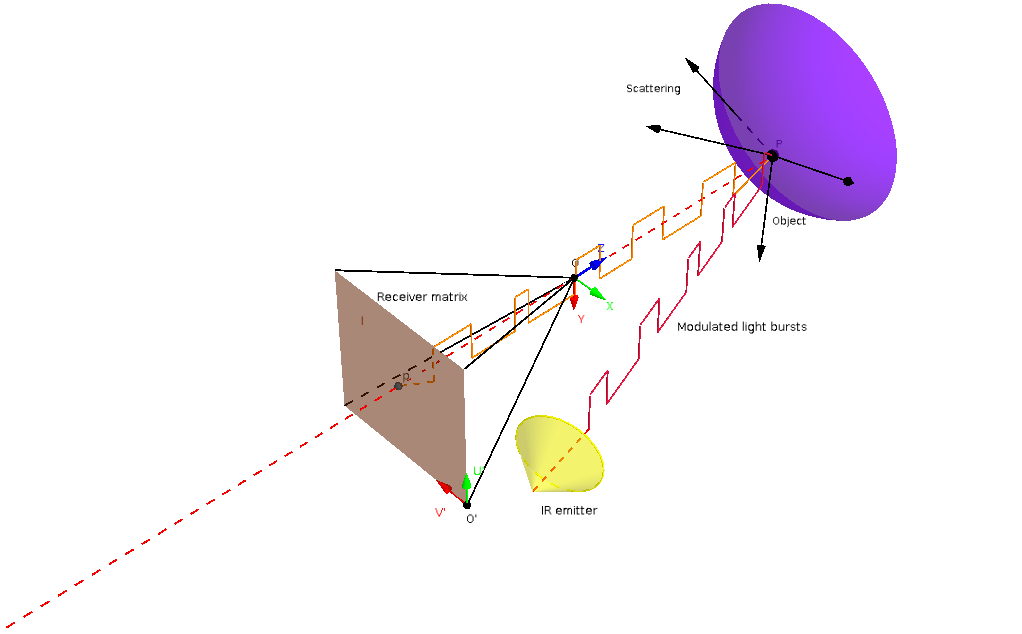
\includegraphics[width=14cm]{img/cam_orf.png}
		\caption{Principle of a time-of-flight camera. The pinhole model is still applicable for the geometry but the measurement of the phase allows to create a new image: the \textit{depth map} $D_T$}
		\label{fig:cam_orf}
	\end{center}
\end{figure}

In addition to the \textit{depth map} $D_T$, two other images can be extracted from the sensor. In figure \ref{fig:cam_orf_2} provided by the Data Sheet of the camera, we are using \cite{SR4k_manual}, $A$ is a measure of the modulated signal amplitude and helps to compute a \textit{confidence map} $C_T$ (the larger $A$, the better confidence on the measure); $B$ is a measure of the mean signal amplitude and gives a \textit{visual image} $V_T$ very similar to the one we can have with traditional black and white cameras.

% Figure cam_orf_2
\begin{figure}[!htt]
	\begin{center}
		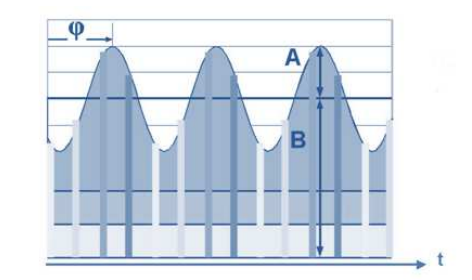
\includegraphics[width=12cm]{img/cam_orf_2.png}
		\caption{The received modulated IR signal is sampled and three images can be computed from the parameters $A$, $B$ and $\Delta \phi$: \textit{depth map} $D_T$, \textit{confidence map} $C_T$ and \textit{visual image} $V_T$ - \textit{Mesa Imaging SR4k Data Sheet \cite{SR4k_manual}}}
		\label{fig:cam_orf_2}
	\end{center}
\end{figure}




\section{Calibration Algorithm}
\label{sec:calib}
\subsection{Literature Overview}
The calibration is a process that aims at finding the most accurate \textit{instrinsic} and \textit{extrinsic} matrices of the pinhole model described in sections \ref{sec:mono_camera} and \ref{sec:stereo_camera} without any prior knowledge of the camera geometry. A precise camera calibration constitutes an important problem since it determines the accuracy of the results. Thus, numerous alternate methods have been developed to guarantee the best possible calibration. According to \cite{intrinsic_calib}, this process can be divided into three categories:
\begin{itemize*}
\item \textbf{3D object-based calibration}: The known geometry of a 3D object as well as its projection are used to compute the best matrices that verify the pinhole equation \ref{eq:pinhole}. It however requires the presence of an accurate 3D calibration target for each calibration.
\item \textbf{Self-calibration}: No object is used but the rigidity of a static environment induces enough constraints to estimate the calibration parameters. If this is very flexible, it is still not always reliable as a lot of initial parameters has to be estimated.
\item \textbf{2D pattern-based calibration}: This third category is a compromise of flexibility (it requires only a 2D pattern like a checkerboard) and reliability (the solution always converges).
\end{itemize*}
\subsubsection{\gls{ORF} calibration}
Calibrating the \gls{ORF} can be seen as a single camera calibration as it involves only the estimation of the \textit{intrinsic matrix}. Different methods has been proposed in \cite{tof_calibration} or \cite{tof_calibration_2}. Due to its success, the Brown method presented in \cite{intrinsic_calib} and \cite{intrinsic_calib_1} will be considered. 
Apart from the \textit{intrinsic} calibration, we shall however notice that \cite{stereo_tof_fusion_proba} and \cite{tof_calibration_1} explain that we shall correct the systematic depth measurement error and this can be realized with a polynomial correction functional approach.
\subsubsection{Stereoscopic cameras calibration}
This category is relatively old, which is an advantage since we can find numerous efficient ways to realize them in the literature. For example, in the \gls{VERTIGO} project, the Brown method \cite{camera_distortion} has been tested through the \textit{OpenCV} libraries \cite{opencv} leading to satisfying results \cite{vertigo_phd}.
\subsubsection{\gls{ORF}-stereo system calibration}
This last category aims at finding \textit{extrinsic matrices} between the \gls{ORF} camera and the stereo cameras assembly. Since the problem is quite recent, different algorithms have been proposed these last few years in \cite{stereo_tof_fusion_proba}, \cite{stereo_tof_fusion_accuracy}, \cite{tof_calibration_1}. In this paper, we will focus on the algorithm presented in \cite{stereo_tof_fusion_proba} because besides the \gls{ORF} \textit{visual image} whose space resolution is very low, the process also takes profit of the \textit{depth map} to increase the accuracy.


\subsection{Optical Range Finder Calibration}
As the \gls{ORF} can be seen as a simple camera, the goal of the process is to find the matrix $K$ in the pinhole equation:
\begin{equation}
s \begin{pmatrix}[0.8]
u_T\\
v_T\\
1
\end{pmatrix}
 = K * \begin{pmatrix}[0.8]
 x_T\\
 y_T\\
 z_T\\
 1
 	\end{pmatrix}
\end{equation}
Let's take a set of world points $P_T^i$ ($i=1...m$) and their projection $p_T^i$. For each $i$, this equation ca be rewritten:
\begin{equation}
\label{eq:K}
p_T^i = \begin{pmatrix}[0.8]
u\\
v
\end{pmatrix}_T^i =  \mathcal{K}(f_U, f_V, c_U, c_V, s_{UV}, P_T^i)
\end{equation}
If we consider now the distortion model proposed in \cite{camera_distortion}, we can match initial coordinates $(u_{init},v_{init})$ in the \textit{image plan} with \textit{undistorted} coordinates $(u_{corr}, v_{corr})$ in the same plan through the equation:
\begin{equation}
\label{eq:D}
p_{corr}^i = \begin{pmatrix}[0.8]
u\\
v
\end{pmatrix}_{corr}^i =  \mathcal{D}(u_{init}^i, v_{init}^i, k_1, k_2, k_3, k_4, k_5)
\end{equation}
Where:
\begin{equation}
	\begin{cases}
		u_{corr} = u * (1 + k_1 r + k_2 r^4 + k_3 r^6) + 2 k_4 u v_ + k_5 (r^2 + 2 u^2)\\
		v_{corr} = v * (1 + k_1 r + k_2 r^4 + k_3 r^6) + k_4 (r^2 + 2 v^2) + 2 k_5 u v\\
		r = \sqrt{u + v}\\
		u = \dfrac{u_{init}}{z}\\
		v = \dfrac{v_{init}}{z}\\
	\end{cases}
\end{equation}
From \ref{eq:K} and \ref{eq:D}, we can write then:
\begin{equation}
\label{eq:F}
p_T^i = \begin{pmatrix}[0.8]
u\\
v
\end{pmatrix}_T^i =  \mathcal{F}(f_U, f_V, c_U, c_V, s_{UV}, k_1, k_2, k_3, k_4, k_5, P_T^i)
\end{equation}
Or more simply:
\begin{equation}
\label{eq:F2}
p_T^i =  \mathcal{F}(\theta_T^i)
\end{equation}
If we define $\theta_T^i = (f_U, f_V, c_U, c_V, s_{UV}, k_1, k_2, k_3, k_4, k_5, P_T^i)$ as the unknown vector.

Practically, all those points $P_T^i$ correspond to the points on a plane pattern (the corner of a checkerboard). Therefore, to find the vector $\theta_T^i$, we detect the checkerboard corners projections $p_T^i$ in the \textit{visual image} $V_T$, we create an initial guess $\hat{\theta}_T^i$ for each point and we solve the constrained iterative least square problem:
\begin{equation}
\label{eq:calib_min}
\theta_T^i = \mathtt{arg}\enspace \mathsf{min}\,\bigg\{\sum_{i=1}^m\, \lVert\mathcal{F}(\hat{\theta}_T^i) - p_T^i\rVert^2\bigg\}
\end{equation}
Where constraints are:
\begin{itemize*}
\item \textit{All points are in the same plane}
\item \textit{The distance between two consecutive points is known}
\end{itemize*}
As the iterative algorithm used to solve the problem \ref{eq:calib_min} has been detailed in \cite{intrinsic_calib} and already implemented in OpenCV, we will not go into further details but understanding how the problem is defined will be useful in the following sections.


\subsection{Stereoscopic Cameras Calibration}
In a stereoscopic calibration, the same thought process can be applied as in the previous paragraph except that \textit{intrinsic} and \textit{extrinsic} matrices for both cameras must be estimated in the same time. Indeed, we start from the equation system \ref{eq:stereo}, which gives after rewriting:
\begin{equation}
\label{eq:F_stero}
\begin{pmatrix}[0.8]
	p_L\\
	p_R
\end{pmatrix}^i
=  \mathcal{F}_{stereo}(\theta_{stereo})
\end{equation}
Where:
\begin{equation}
\theta_{stereo} = \begin{pmatrix}[0.8]
f_U^L, f_V^L, c_U^L, c_V^L, s_{UV}^L, k_1^L, k_2^L, k_3^L, k_4^L, k_5^L, P_L^i\\
f_U^R, f_V^R, c_U^R, c_V^R, s_{UV}^R, k_1^R, k_2^R, k_3^R, k_4^R, k_5^R, P_R^i\\
M_LR
\end{pmatrix}
\end{equation}
The minimization problem is then:
\begin{equation}
\label{eq:calib_min_stereo}
\theta_{stereo}^i = \mathtt{arg}\enspace \mathsf{min}\,\bigg\{\sum_{i=1}^m\, \bigg\lVert\mathcal{F}_{stereo}(\hat{\theta}_{stereo}^i)
- \begin{pmatrix}[0.8]
p_L\\
p_R
\end{pmatrix}^i\bigg\rVert^2\bigg\}
\end{equation}
The constraints are now:
\begin{itemize*}
\item \textit{All points are in the same plane}
\item \textit{The distance between two consecutive points is known}
\item \textit{Two epipolar lines cross in one single point (or the error is minimized in the case of a complex model)}
\end{itemize*}

\subsection{Multi-Sensors Calibration}
\label{subsec:system_calib}
In this third and last part of calibration, we focused on the estimation of the extrinsic matrix between the \gls{ORF} and the stereoscopic cameras. As  explained in the literature review, this method proposed in \cite{stereo_tof_fusion_proba} takes advantage of all the information given by the sensors and not only of visual images. Figure \ref{fig:calib_arch} shows the architecture of this method and theoretical details are given in the following paragraphs.

% Figure calib_arch
\begin{figure}[!htt] 
	\begin{center}
		{\scalefont{0.5}
		% Graphic for TeX using PGF
% Title: /home/gabs48/mit/thesis/graphic/calib_arch.dia
% Creator: Dia v0.97.2
% CreationDate: Fri Oct 10 14:03:20 2014
% For: gabs48
% \usepackage{tikz}
% The following commands are not supported in PSTricks at present
% We define them conditionally, so when they are implemented,
% this pgf file will use them.
\ifx\du\undefined
  \newlength{\du}
\fi
\setlength{\du}{15\unitlength}
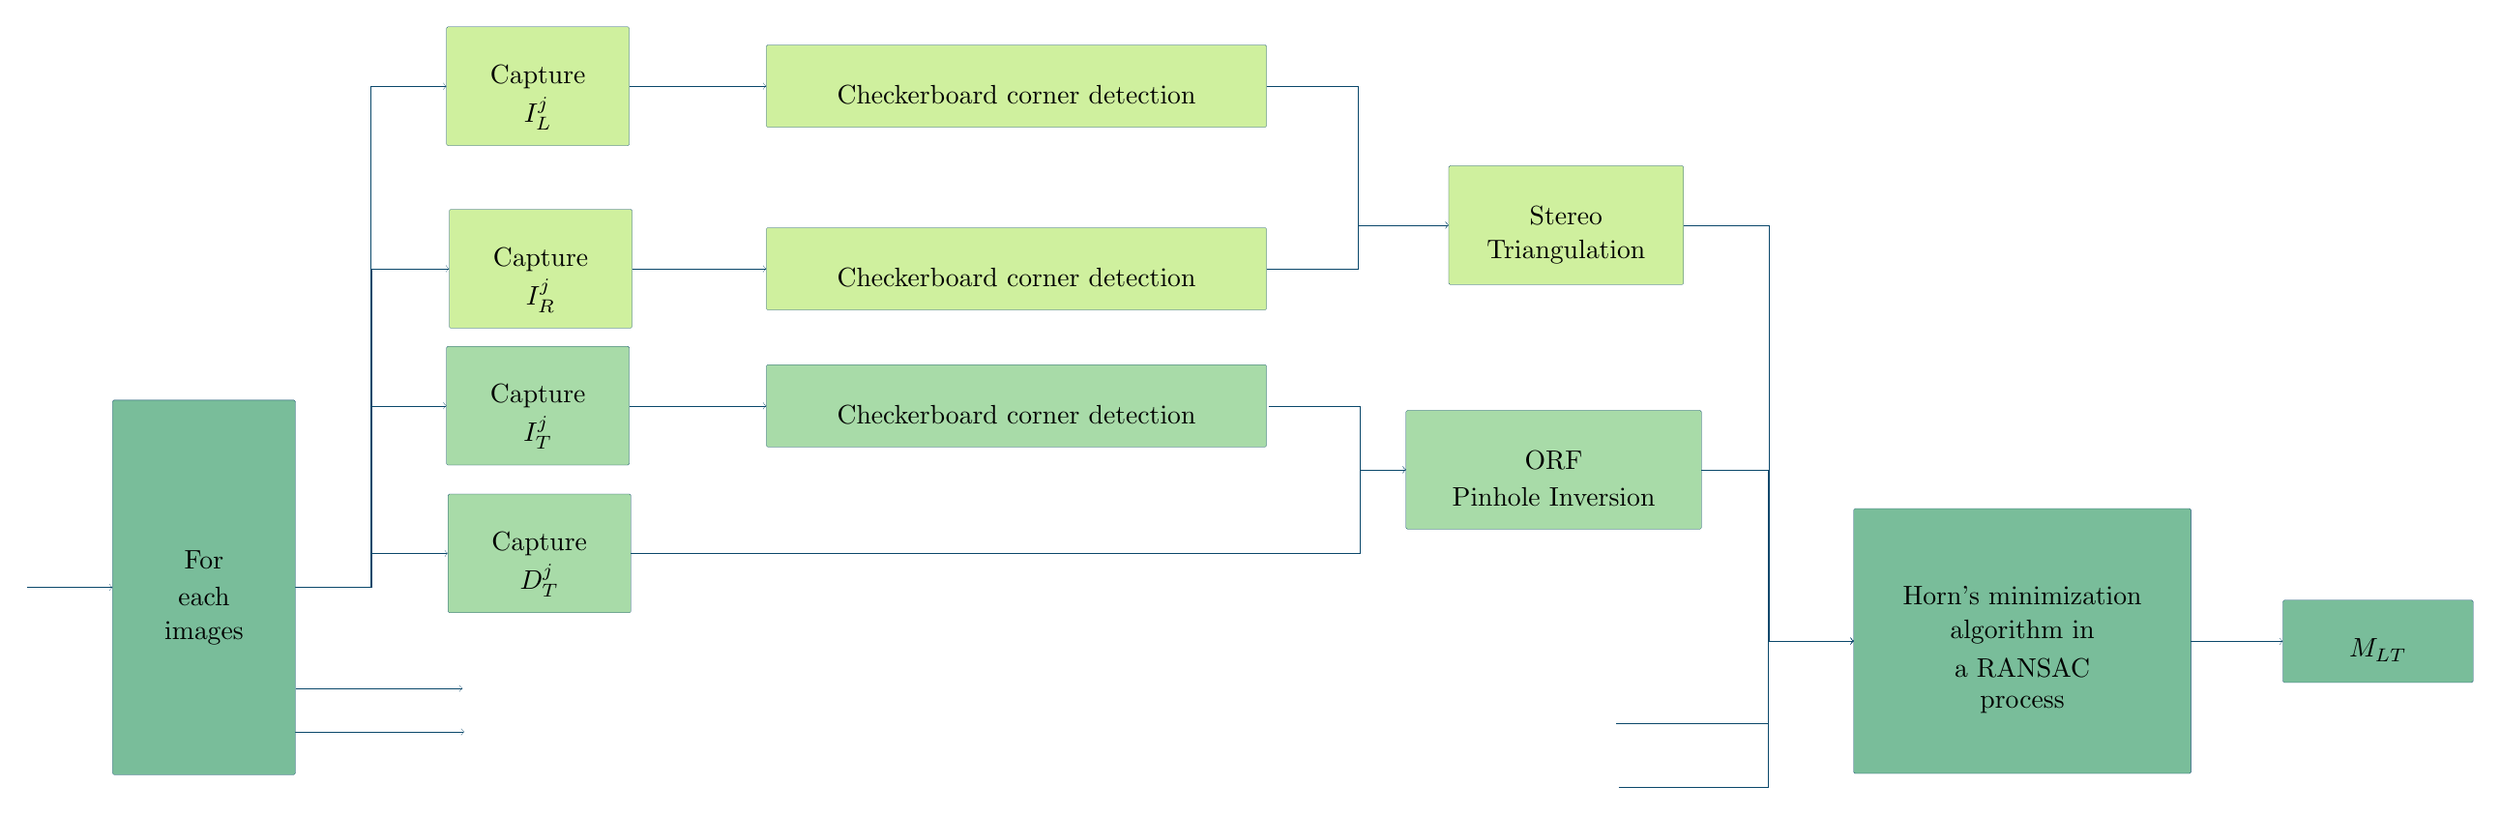
\begin{tikzpicture}
\pgftransformxscale{0.600000}
\pgftransformyscale{-0.600000}
\definecolor{dialinecolor}{rgb}{0.000000, 0.000000, 0.000000}
\pgfsetstrokecolor{dialinecolor}
\definecolor{dialinecolor}{rgb}{1.000000, 1.000000, 1.000000}
\pgfsetfillcolor{dialinecolor}
\pgfsetlinewidth{0.100000\du}
\pgfsetdash{}{0pt}
{\pgfsetcornersarced{\pgfpoint{0.500000\du}{0.500000\du}}\definecolor{dialinecolor}{rgb}{0.811765, 0.941176, 0.619608}
\pgfsetfillcolor{dialinecolor}
\fill (15.000000\du,11.000000\du)--(15.000000\du,12.800000\du)--(25.947500\du,12.800000\du)--(25.947500\du,11.000000\du)--cycle;
}{\pgfsetcornersarced{\pgfpoint{0.500000\du}{0.500000\du}}\definecolor{dialinecolor}{rgb}{0.043137, 0.282353, 0.419608}
\pgfsetstrokecolor{dialinecolor}
\draw (15.000000\du,11.000000\du)--(15.000000\du,12.800000\du)--(25.947500\du,12.800000\du)--(25.947500\du,11.000000\du)--cycle;
}% setfont left to latex
\definecolor{dialinecolor}{rgb}{0.043137, 0.282353, 0.419608}
\pgfsetstrokecolor{dialinecolor}
\node at (20.473750\du,12.095000\du){Checkerboard corner detection};
\pgfsetlinewidth{0.100000\du}
\pgfsetdash{}{0pt}
{\pgfsetcornersarced{\pgfpoint{0.500000\du}{0.500000\du}}\definecolor{dialinecolor}{rgb}{0.811765, 0.941176, 0.619608}
\pgfsetfillcolor{dialinecolor}
\fill (15.000000\du,15.000000\du)--(15.000000\du,16.800000\du)--(25.947500\du,16.800000\du)--(25.947500\du,15.000000\du)--cycle;
}{\pgfsetcornersarced{\pgfpoint{0.500000\du}{0.500000\du}}\definecolor{dialinecolor}{rgb}{0.043137, 0.282353, 0.419608}
\pgfsetstrokecolor{dialinecolor}
\draw (15.000000\du,15.000000\du)--(15.000000\du,16.800000\du)--(25.947500\du,16.800000\du)--(25.947500\du,15.000000\du)--cycle;
}% setfont left to latex
\definecolor{dialinecolor}{rgb}{0.043137, 0.282353, 0.419608}
\pgfsetstrokecolor{dialinecolor}
\node at (20.473750\du,16.095000\du){Checkerboard corner detection};
\pgfsetlinewidth{0.100000\du}
\pgfsetdash{}{0pt}
{\pgfsetcornersarced{\pgfpoint{0.500000\du}{0.500000\du}}\definecolor{dialinecolor}{rgb}{0.658824, 0.858824, 0.658824}
\pgfsetfillcolor{dialinecolor}
\fill (15.000000\du,18.000000\du)--(15.000000\du,19.800000\du)--(25.947500\du,19.800000\du)--(25.947500\du,18.000000\du)--cycle;
}{\pgfsetcornersarced{\pgfpoint{0.500000\du}{0.500000\du}}\definecolor{dialinecolor}{rgb}{0.043137, 0.282353, 0.419608}
\pgfsetstrokecolor{dialinecolor}
\draw (15.000000\du,18.000000\du)--(15.000000\du,19.800000\du)--(25.947500\du,19.800000\du)--(25.947500\du,18.000000\du)--cycle;
}% setfont left to latex
\definecolor{dialinecolor}{rgb}{0.043137, 0.282353, 0.419608}
\pgfsetstrokecolor{dialinecolor}
\node at (20.473750\du,19.095000\du){Checkerboard corner detection};
\pgfsetlinewidth{0.100000\du}
\pgfsetdash{}{0pt}
{\pgfsetcornersarced{\pgfpoint{0.500000\du}{0.500000\du}}\definecolor{dialinecolor}{rgb}{0.658824, 0.858824, 0.658824}
\pgfsetfillcolor{dialinecolor}
\fill (29.000000\du,19.000000\du)--(29.000000\du,21.600000\du)--(35.465000\du,21.600000\du)--(35.465000\du,19.000000\du)--cycle;
}{\pgfsetcornersarced{\pgfpoint{0.500000\du}{0.500000\du}}\definecolor{dialinecolor}{rgb}{0.043137, 0.282353, 0.419608}
\pgfsetstrokecolor{dialinecolor}
\draw (29.000000\du,19.000000\du)--(29.000000\du,21.600000\du)--(35.465000\du,21.600000\du)--(35.465000\du,19.000000\du)--cycle;
}% setfont left to latex
\definecolor{dialinecolor}{rgb}{0.043137, 0.282353, 0.419608}
\pgfsetstrokecolor{dialinecolor}
\node at (32.232500\du,20.095000\du){ORF};
% setfont left to latex
\definecolor{dialinecolor}{rgb}{0.043137, 0.282353, 0.419608}
\pgfsetstrokecolor{dialinecolor}
\node at (32.232500\du,20.895000\du){Pinhole Inversion};
\pgfsetlinewidth{0.100000\du}
\pgfsetbuttcap
\pgfsetdash{}{0pt}
{
\definecolor{dialinecolor}{rgb}{0.043137, 0.282353, 0.419608}
\pgfsetfillcolor{dialinecolor}
% was here!!!
\pgfsetarrowsend{to}
\definecolor{dialinecolor}{rgb}{0.043137, 0.282353, 0.419608}
\pgfsetstrokecolor{dialinecolor}
\draw (25.947500\du,11.900000\du)--(27.941049\du,11.900000\du)--(27.941049\du,14.944005\du)--(29.934598\du,14.944005\du);
}
% setfont left to latex
\pgfsetlinewidth{0.100000\du}
\pgfsetbuttcap
\pgfsetdash{}{0pt}
{
\definecolor{dialinecolor}{rgb}{0.043137, 0.282353, 0.419608}
\pgfsetfillcolor{dialinecolor}
% was here!!!
\pgfsetarrowsend{to}
\definecolor{dialinecolor}{rgb}{0.043137, 0.282353, 0.419608}
\pgfsetstrokecolor{dialinecolor}
\draw (25.947500\du,15.900000\du)--(27.941049\du,15.900000\du)--(27.941049\du,14.944005\du)--(29.934598\du,14.944005\du);
}
% setfont left to latex
\pgfsetlinewidth{0.100000\du}
\pgfsetbuttcap
\pgfsetdash{}{0pt}
{
\definecolor{dialinecolor}{rgb}{0.043137, 0.282353, 0.419608}
\pgfsetfillcolor{dialinecolor}
% was here!!!
\pgfsetarrowsend{to}
\definecolor{dialinecolor}{rgb}{0.043137, 0.282353, 0.419608}
\pgfsetstrokecolor{dialinecolor}
\draw (25.997624\du,18.900000\du)--(28.000000\du,18.900000\du)--(28.000000\du,20.300000\du)--(29.000000\du,20.300000\du);
}
% setfont left to latex
\pgfsetlinewidth{0.100000\du}
\pgfsetbuttcap
\pgfsetdash{}{0pt}
{
\definecolor{dialinecolor}{rgb}{0.043137, 0.282353, 0.419608}
\pgfsetfillcolor{dialinecolor}
% was here!!!
\pgfsetarrowsend{to}
\definecolor{dialinecolor}{rgb}{0.043137, 0.282353, 0.419608}
\pgfsetstrokecolor{dialinecolor}
\draw (12.001417\du,11.903914\du)--(13.500708\du,11.903914\du)--(13.500708\du,11.900000\du)--(15.000000\du,11.900000\du);
}
% setfont left to latex
\pgfsetlinewidth{0.100000\du}
\pgfsetbuttcap
\pgfsetdash{}{0pt}
{
\definecolor{dialinecolor}{rgb}{0.043137, 0.282353, 0.419608}
\pgfsetfillcolor{dialinecolor}
% was here!!!
\pgfsetarrowsend{to}
\definecolor{dialinecolor}{rgb}{0.043137, 0.282353, 0.419608}
\pgfsetstrokecolor{dialinecolor}
\draw (12.060496\du,15.898733\du)--(13.525000\du,15.898733\du)--(13.525000\du,15.900000\du)--(15.000000\du,15.900000\du);
}
% setfont left to latex
\pgfsetlinewidth{0.100000\du}
\pgfsetbuttcap
\pgfsetdash{}{0pt}
{
\definecolor{dialinecolor}{rgb}{0.043137, 0.282353, 0.419608}
\pgfsetfillcolor{dialinecolor}
% was here!!!
\pgfsetarrowsend{to}
\definecolor{dialinecolor}{rgb}{0.043137, 0.282353, 0.419608}
\pgfsetstrokecolor{dialinecolor}
\draw (12.001482\du,18.897713\du)--(13.500741\du,18.897713\du)--(13.500741\du,18.900000\du)--(15.000000\du,18.900000\du);
}
% setfont left to latex
\pgfsetlinewidth{0.100000\du}
\pgfsetbuttcap
\pgfsetdash{}{0pt}
{
\definecolor{dialinecolor}{rgb}{0.043137, 0.282353, 0.419608}
\pgfsetfillcolor{dialinecolor}
% was here!!!
\pgfsetarrowsend{to}
\definecolor{dialinecolor}{rgb}{0.043137, 0.282353, 0.419608}
\pgfsetstrokecolor{dialinecolor}
\draw (12.033259\du,22.131456\du)--(28.000000\du,22.131456\du)--(28.000000\du,20.300000\du)--(29.000000\du,20.300000\du);
}
% setfont left to latex
\pgfsetlinewidth{0.100000\du}
\pgfsetdash{}{0pt}
{\pgfsetcornersarced{\pgfpoint{0.500000\du}{0.500000\du}}\definecolor{dialinecolor}{rgb}{0.474510, 0.741176, 0.603922}
\pgfsetfillcolor{dialinecolor}
\fill (38.800000\du,21.150000\du)--(38.800000\du,26.950000\du)--(46.177500\du,26.950000\du)--(46.177500\du,21.150000\du)--cycle;
}{\pgfsetcornersarced{\pgfpoint{0.500000\du}{0.500000\du}}\definecolor{dialinecolor}{rgb}{0.043137, 0.282353, 0.419608}
\pgfsetstrokecolor{dialinecolor}
\draw (38.800000\du,21.150000\du)--(38.800000\du,26.950000\du)--(46.177500\du,26.950000\du)--(46.177500\du,21.150000\du)--cycle;
}% setfont left to latex
\definecolor{dialinecolor}{rgb}{0.043137, 0.282353, 0.419608}
\pgfsetstrokecolor{dialinecolor}
\node at (42.488750\du,22.245000\du){};
% setfont left to latex
\definecolor{dialinecolor}{rgb}{0.043137, 0.282353, 0.419608}
\pgfsetstrokecolor{dialinecolor}
\node at (42.488750\du,23.045000\du){Horn's minimization};
% setfont left to latex
\definecolor{dialinecolor}{rgb}{0.043137, 0.282353, 0.419608}
\pgfsetstrokecolor{dialinecolor}
\node at (42.488750\du,23.845000\du){algorithm in};
% setfont left to latex
\definecolor{dialinecolor}{rgb}{0.043137, 0.282353, 0.419608}
\pgfsetstrokecolor{dialinecolor}
\node at (42.488750\du,24.645000\du){a RANSAC};
% setfont left to latex
\definecolor{dialinecolor}{rgb}{0.043137, 0.282353, 0.419608}
\pgfsetstrokecolor{dialinecolor}
\node at (42.488750\du,25.445000\du){process};
% setfont left to latex
\definecolor{dialinecolor}{rgb}{0.043137, 0.282353, 0.419608}
\pgfsetstrokecolor{dialinecolor}
\node at (42.488750\du,26.245000\du){};
\pgfsetlinewidth{0.100000\du}
\pgfsetbuttcap
\pgfsetdash{}{0pt}
{
\definecolor{dialinecolor}{rgb}{0.043137, 0.282353, 0.419608}
\pgfsetfillcolor{dialinecolor}
% was here!!!
\pgfsetarrowsend{to}
\definecolor{dialinecolor}{rgb}{0.043137, 0.282353, 0.419608}
\pgfsetstrokecolor{dialinecolor}
\draw (35.465000\du,20.300000\du)--(36.917982\du,20.300000\du)--(36.917982\du,24.050000\du)--(38.800000\du,24.050000\du);
}
% setfont left to latex
\pgfsetlinewidth{0.100000\du}
\pgfsetbuttcap
\pgfsetdash{}{0pt}
{
\definecolor{dialinecolor}{rgb}{0.043137, 0.282353, 0.419608}
\pgfsetfillcolor{dialinecolor}
% was here!!!
\pgfsetarrowsend{to}
\definecolor{dialinecolor}{rgb}{0.043137, 0.282353, 0.419608}
\pgfsetstrokecolor{dialinecolor}
\draw (35.074598\du,14.944005\du)--(36.937299\du,14.944005\du)--(36.937299\du,24.050000\du)--(38.800000\du,24.050000\du);
}
% setfont left to latex
\pgfsetlinewidth{0.100000\du}
\pgfsetbuttcap
\pgfsetdash{}{0pt}
{
\definecolor{dialinecolor}{rgb}{0.043137, 0.282353, 0.419608}
\pgfsetfillcolor{dialinecolor}
% was here!!!
\pgfsetarrowsend{to}
\definecolor{dialinecolor}{rgb}{0.043137, 0.282353, 0.419608}
\pgfsetstrokecolor{dialinecolor}
\draw (33.600000\du,25.850000\du)--(36.917982\du,25.850000\du)--(36.917982\du,24.050000\du)--(38.800000\du,24.050000\du);
}
% setfont left to latex
\pgfsetlinewidth{0.100000\du}
\pgfsetbuttcap
\pgfsetdash{}{0pt}
{
\definecolor{dialinecolor}{rgb}{0.043137, 0.282353, 0.419608}
\pgfsetfillcolor{dialinecolor}
% was here!!!
\pgfsetarrowsend{to}
\definecolor{dialinecolor}{rgb}{0.043137, 0.282353, 0.419608}
\pgfsetstrokecolor{dialinecolor}
\draw (33.650000\du,27.250000\du)--(36.917982\du,27.250000\du)--(36.917982\du,24.050000\du)--(38.800000\du,24.050000\du);
}
% setfont left to latex
\pgfsetlinewidth{0.100000\du}
\pgfsetbuttcap
\pgfsetdash{}{0pt}
{
\definecolor{dialinecolor}{rgb}{0.043137, 0.282353, 0.419608}
\pgfsetfillcolor{dialinecolor}
% was here!!!
\pgfsetarrowsend{to}
\definecolor{dialinecolor}{rgb}{0.043137, 0.282353, 0.419608}
\pgfsetstrokecolor{dialinecolor}
\draw (46.177500\du,24.050000\du)--(47.184333\du,24.050000\du)--(47.184333\du,24.056152\du)--(48.191166\du,24.056152\du);
}
% setfont left to latex
\pgfsetlinewidth{0.100000\du}
\pgfsetbuttcap
\pgfsetdash{}{0pt}
{
\definecolor{dialinecolor}{rgb}{0.043137, 0.282353, 0.419608}
\pgfsetfillcolor{dialinecolor}
% was here!!!
\pgfsetarrowsend{to}
\definecolor{dialinecolor}{rgb}{0.043137, 0.282353, 0.419608}
\pgfsetstrokecolor{dialinecolor}
\draw (4.692174\du,22.875052\du)--(6.346795\du,22.875052\du)--(6.346795\du,11.903914\du)--(8.001417\du,11.903914\du);
}
% setfont left to latex
\pgfsetlinewidth{0.100000\du}
\pgfsetbuttcap
\pgfsetdash{}{0pt}
{
\definecolor{dialinecolor}{rgb}{0.043137, 0.282353, 0.419608}
\pgfsetfillcolor{dialinecolor}
% was here!!!
\pgfsetarrowsend{to}
\definecolor{dialinecolor}{rgb}{0.043137, 0.282353, 0.419608}
\pgfsetstrokecolor{dialinecolor}
\draw (4.692174\du,22.875052\du)--(6.354436\du,22.875052\du)--(6.354436\du,15.898733\du)--(8.060496\du,15.898733\du);
}
% setfont left to latex
\pgfsetlinewidth{0.100000\du}
\pgfsetbuttcap
\pgfsetdash{}{0pt}
{
\definecolor{dialinecolor}{rgb}{0.043137, 0.282353, 0.419608}
\pgfsetfillcolor{dialinecolor}
% was here!!!
\pgfsetarrowsend{to}
\definecolor{dialinecolor}{rgb}{0.043137, 0.282353, 0.419608}
\pgfsetstrokecolor{dialinecolor}
\draw (4.692174\du,22.875052\du)--(6.346828\du,22.875052\du)--(6.346828\du,18.897713\du)--(8.001482\du,18.897713\du);
}
% setfont left to latex
\pgfsetlinewidth{0.100000\du}
\pgfsetbuttcap
\pgfsetdash{}{0pt}
{
\definecolor{dialinecolor}{rgb}{0.043137, 0.282353, 0.419608}
\pgfsetfillcolor{dialinecolor}
% was here!!!
\pgfsetarrowsend{to}
\definecolor{dialinecolor}{rgb}{0.043137, 0.282353, 0.419608}
\pgfsetstrokecolor{dialinecolor}
\draw (4.692174\du,22.875052\du)--(6.354436\du,22.875052\du)--(6.354436\du,22.131456\du)--(8.033259\du,22.131456\du);
}
% setfont left to latex
\pgfsetlinewidth{0.100000\du}
\pgfsetbuttcap
\pgfsetdash{}{0pt}
{
\definecolor{dialinecolor}{rgb}{0.043137, 0.282353, 0.419608}
\pgfsetfillcolor{dialinecolor}
% was here!!!
\pgfsetarrowsend{to}
\definecolor{dialinecolor}{rgb}{0.043137, 0.282353, 0.419608}
\pgfsetstrokecolor{dialinecolor}
\draw (4.695407\du,25.085925\du)--(6.523887\du,25.085925\du)--(6.523887\du,25.086641\du)--(8.352366\du,25.086641\du);
}
% setfont left to latex
\pgfsetlinewidth{0.100000\du}
\pgfsetbuttcap
\pgfsetdash{}{0pt}
{
\definecolor{dialinecolor}{rgb}{0.043137, 0.282353, 0.419608}
\pgfsetfillcolor{dialinecolor}
% was here!!!
\pgfsetarrowsend{to}
\definecolor{dialinecolor}{rgb}{0.043137, 0.282353, 0.419608}
\pgfsetstrokecolor{dialinecolor}
\draw (4.650000\du,26.038761\du)--(6.521277\du,26.038761\du)--(6.521277\du,26.038729\du)--(8.392555\du,26.038729\du);
}
% setfont left to latex
% setfont left to latex
\definecolor{dialinecolor}{rgb}{0.043137, 0.282353, 0.419608}
\pgfsetstrokecolor{dialinecolor}
\node[anchor=west] at (2.620301\du,20.636790\du){};
\pgfsetlinewidth{0.100000\du}
\pgfsetbuttcap
\pgfsetdash{}{0pt}
{
\definecolor{dialinecolor}{rgb}{0.043137, 0.282353, 0.419608}
\pgfsetfillcolor{dialinecolor}
% was here!!!
\pgfsetarrowsend{to}
\definecolor{dialinecolor}{rgb}{0.043137, 0.282353, 0.419608}
\pgfsetstrokecolor{dialinecolor}
\draw (-1.183208\du,22.861674\du)--(-0.149038\du,22.861674\du)--(-0.149038\du,22.875052\du)--(0.692174\du,22.875052\du);
}
% setfont left to latex
\pgfsetlinewidth{0.100000\du}
\pgfsetdash{}{0pt}
{\pgfsetcornersarced{\pgfpoint{0.500000\du}{0.500000\du}}\definecolor{dialinecolor}{rgb}{0.474510, 0.741176, 0.603922}
\pgfsetfillcolor{dialinecolor}
\fill (0.692174\du,18.775052\du)--(0.692174\du,26.975052\du)--(4.692174\du,26.975052\du)--(4.692174\du,18.775052\du)--cycle;
}{\pgfsetcornersarced{\pgfpoint{0.500000\du}{0.500000\du}}\definecolor{dialinecolor}{rgb}{0.043137, 0.282353, 0.419608}
\pgfsetstrokecolor{dialinecolor}
\draw (0.692174\du,18.775052\du)--(0.692174\du,26.975052\du)--(4.692174\du,26.975052\du)--(4.692174\du,18.775052\du)--cycle;
}% setfont left to latex
\definecolor{dialinecolor}{rgb}{0.043137, 0.282353, 0.419608}
\pgfsetstrokecolor{dialinecolor}
\node at (2.692174\du,19.870052\du){};
% setfont left to latex
\definecolor{dialinecolor}{rgb}{0.043137, 0.282353, 0.419608}
\pgfsetstrokecolor{dialinecolor}
\node at (2.692174\du,20.670052\du){};
% setfont left to latex
\definecolor{dialinecolor}{rgb}{0.043137, 0.282353, 0.419608}
\pgfsetstrokecolor{dialinecolor}
\node at (2.692174\du,21.470052\du){};
% setfont left to latex
\definecolor{dialinecolor}{rgb}{0.043137, 0.282353, 0.419608}
\pgfsetstrokecolor{dialinecolor}
\node at (2.692174\du,22.270052\du){For};
% setfont left to latex
\definecolor{dialinecolor}{rgb}{0.043137, 0.282353, 0.419608}
\pgfsetstrokecolor{dialinecolor}
\node at (2.692174\du,23.070052\du){each};
% setfont left to latex
\definecolor{dialinecolor}{rgb}{0.043137, 0.282353, 0.419608}
\pgfsetstrokecolor{dialinecolor}
\node at (2.692174\du,23.870052\du){images};
% setfont left to latex
\definecolor{dialinecolor}{rgb}{0.043137, 0.282353, 0.419608}
\pgfsetstrokecolor{dialinecolor}
\node at (2.692174\du,24.670052\du){};
% setfont left to latex
\definecolor{dialinecolor}{rgb}{0.043137, 0.282353, 0.419608}
\pgfsetstrokecolor{dialinecolor}
\node at (2.692174\du,25.470052\du){};
% setfont left to latex
\definecolor{dialinecolor}{rgb}{0.043137, 0.282353, 0.419608}
\pgfsetstrokecolor{dialinecolor}
\node at (2.692174\du,26.270052\du){};
\pgfsetlinewidth{0.100000\du}
\pgfsetdash{}{0pt}
{\pgfsetcornersarced{\pgfpoint{0.500000\du}{0.500000\du}}\definecolor{dialinecolor}{rgb}{0.811765, 0.941176, 0.619608}
\pgfsetfillcolor{dialinecolor}
\fill (29.934598\du,13.644005\du)--(29.934598\du,16.244005\du)--(35.074598\du,16.244005\du)--(35.074598\du,13.644005\du)--cycle;
}{\pgfsetcornersarced{\pgfpoint{0.500000\du}{0.500000\du}}\definecolor{dialinecolor}{rgb}{0.043137, 0.282353, 0.419608}
\pgfsetstrokecolor{dialinecolor}
\draw (29.934598\du,13.644005\du)--(29.934598\du,16.244005\du)--(35.074598\du,16.244005\du)--(35.074598\du,13.644005\du)--cycle;
}% setfont left to latex
\definecolor{dialinecolor}{rgb}{0.043137, 0.282353, 0.419608}
\pgfsetstrokecolor{dialinecolor}
\node at (32.504598\du,14.739005\du){Stereo};
% setfont left to latex
\definecolor{dialinecolor}{rgb}{0.043137, 0.282353, 0.419608}
\pgfsetstrokecolor{dialinecolor}
\node at (32.504598\du,15.539005\du){Triangulation};
\pgfsetlinewidth{0.100000\du}
\pgfsetdash{}{0pt}
{\pgfsetcornersarced{\pgfpoint{0.500000\du}{0.500000\du}}\definecolor{dialinecolor}{rgb}{0.811765, 0.941176, 0.619608}
\pgfsetfillcolor{dialinecolor}
\fill (8.001417\du,10.603914\du)--(8.001417\du,13.203914\du)--(12.001417\du,13.203914\du)--(12.001417\du,10.603914\du)--cycle;
}{\pgfsetcornersarced{\pgfpoint{0.500000\du}{0.500000\du}}\definecolor{dialinecolor}{rgb}{0.043137, 0.282353, 0.419608}
\pgfsetstrokecolor{dialinecolor}
\draw (8.001417\du,10.603914\du)--(8.001417\du,13.203914\du)--(12.001417\du,13.203914\du)--(12.001417\du,10.603914\du)--cycle;
}% setfont left to latex
\definecolor{dialinecolor}{rgb}{0.043137, 0.282353, 0.419608}
\pgfsetstrokecolor{dialinecolor}
\node at (10.001417\du,11.698914\du){Capture};
% setfont left to latex
\definecolor{dialinecolor}{rgb}{0.043137, 0.282353, 0.419608}
\pgfsetstrokecolor{dialinecolor}
\node at (10.001417\du,12.498914\du){$I_L^j$};
\pgfsetlinewidth{0.100000\du}
\pgfsetdash{}{0pt}
{\pgfsetcornersarced{\pgfpoint{0.500000\du}{0.500000\du}}\definecolor{dialinecolor}{rgb}{0.811765, 0.941176, 0.619608}
\pgfsetfillcolor{dialinecolor}
\fill (8.060496\du,14.598733\du)--(8.060496\du,17.198733\du)--(12.060496\du,17.198733\du)--(12.060496\du,14.598733\du)--cycle;
}{\pgfsetcornersarced{\pgfpoint{0.500000\du}{0.500000\du}}\definecolor{dialinecolor}{rgb}{0.043137, 0.282353, 0.419608}
\pgfsetstrokecolor{dialinecolor}
\draw (8.060496\du,14.598733\du)--(8.060496\du,17.198733\du)--(12.060496\du,17.198733\du)--(12.060496\du,14.598733\du)--cycle;
}% setfont left to latex
\definecolor{dialinecolor}{rgb}{0.043137, 0.282353, 0.419608}
\pgfsetstrokecolor{dialinecolor}
\node at (10.060496\du,15.693733\du){Capture};
% setfont left to latex
\definecolor{dialinecolor}{rgb}{0.043137, 0.282353, 0.419608}
\pgfsetstrokecolor{dialinecolor}
\node at (10.060496\du,16.493733\du){$I_R^j$};
\pgfsetlinewidth{0.100000\du}
\pgfsetdash{}{0pt}
{\pgfsetcornersarced{\pgfpoint{0.500000\du}{0.500000\du}}\definecolor{dialinecolor}{rgb}{0.658824, 0.858824, 0.658824}
\pgfsetfillcolor{dialinecolor}
\fill (8.001482\du,17.597713\du)--(8.001482\du,20.197713\du)--(12.001482\du,20.197713\du)--(12.001482\du,17.597713\du)--cycle;
}{\pgfsetcornersarced{\pgfpoint{0.500000\du}{0.500000\du}}\definecolor{dialinecolor}{rgb}{0.043137, 0.282353, 0.419608}
\pgfsetstrokecolor{dialinecolor}
\draw (8.001482\du,17.597713\du)--(8.001482\du,20.197713\du)--(12.001482\du,20.197713\du)--(12.001482\du,17.597713\du)--cycle;
}% setfont left to latex
\definecolor{dialinecolor}{rgb}{0.043137, 0.282353, 0.419608}
\pgfsetstrokecolor{dialinecolor}
\node at (10.001482\du,18.692713\du){Capture};
% setfont left to latex
\definecolor{dialinecolor}{rgb}{0.043137, 0.282353, 0.419608}
\pgfsetstrokecolor{dialinecolor}
\node at (10.001482\du,19.492713\du){$I_T^j$};
\pgfsetlinewidth{0.100000\du}
\pgfsetdash{}{0pt}
{\pgfsetcornersarced{\pgfpoint{0.500000\du}{0.500000\du}}\definecolor{dialinecolor}{rgb}{0.658824, 0.858824, 0.658824}
\pgfsetfillcolor{dialinecolor}
\fill (8.033259\du,20.831456\du)--(8.033259\du,23.431456\du)--(12.033259\du,23.431456\du)--(12.033259\du,20.831456\du)--cycle;
}{\pgfsetcornersarced{\pgfpoint{0.500000\du}{0.500000\du}}\definecolor{dialinecolor}{rgb}{0.043137, 0.282353, 0.419608}
\pgfsetstrokecolor{dialinecolor}
\draw (8.033259\du,20.831456\du)--(8.033259\du,23.431456\du)--(12.033259\du,23.431456\du)--(12.033259\du,20.831456\du)--cycle;
}% setfont left to latex
\definecolor{dialinecolor}{rgb}{0.043137, 0.282353, 0.419608}
\pgfsetstrokecolor{dialinecolor}
\node at (10.033259\du,21.926456\du){Capture};
% setfont left to latex
\definecolor{dialinecolor}{rgb}{0.043137, 0.282353, 0.419608}
\pgfsetstrokecolor{dialinecolor}
\node at (10.033259\du,22.726456\du){$D_T^j$};
\pgfsetlinewidth{0.100000\du}
\pgfsetdash{}{0pt}
{\pgfsetcornersarced{\pgfpoint{0.500000\du}{0.500000\du}}\definecolor{dialinecolor}{rgb}{0.474510, 0.741176, 0.603922}
\pgfsetfillcolor{dialinecolor}
\fill (48.191166\du,23.156152\du)--(48.191166\du,24.956152\du)--(52.353666\du,24.956152\du)--(52.353666\du,23.156152\du)--cycle;
}{\pgfsetcornersarced{\pgfpoint{0.500000\du}{0.500000\du}}\definecolor{dialinecolor}{rgb}{0.043137, 0.282353, 0.419608}
\pgfsetstrokecolor{dialinecolor}
\draw (48.191166\du,23.156152\du)--(48.191166\du,24.956152\du)--(52.353666\du,24.956152\du)--(52.353666\du,23.156152\du)--cycle;
}% setfont left to latex
\definecolor{dialinecolor}{rgb}{0.043137, 0.282353, 0.419608}
\pgfsetstrokecolor{dialinecolor}
\node at (50.272416\du,24.251152\du){$M_{LT}$};
\end{tikzpicture}

		}
	\end{center}
	\caption{Architecture of the multi-sensors extrinsic calibration algorithm}\label{fig:calib_arch}
\end{figure}

\subsubsection{Checkerboard Corners Detection}
Let us consider a system composed by two traditional cameras $L$ and $R$ and an \gls{ORF} (or \gls{ToF}) camera $T$ (figure \ref{fig:3cam}). To keep this method universal, no hypothesis are made on the geometry between those cameras. $L$ and $R$ cameras produce respectively an image matrix $I_L$ and $I_R$ whose resolution is good and $T$ produce a depth matrix $D_T$, a visual image matrix $I_T$ and a confidence matrix $C_T$.

% figure 3cam
\begin{figure}[!htt]
	\begin{center}
		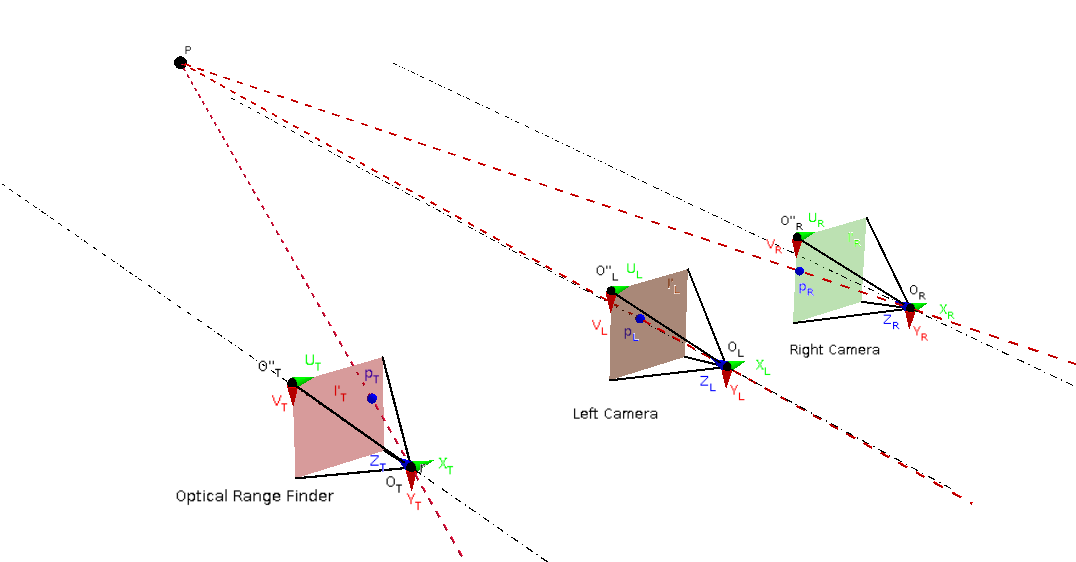
\includegraphics[width=14cm]{img/cam_3.png}
		\caption{A point P of the real world is framed by three cameras: the \gls{ORF}, left camera and right camera}
		\label{fig:3cam}
	\end{center}
\end{figure}

First, the intrinsic parameters of $L$, $R$ and $T$ and the extrinsic parameters between $L$ and $R$ are computed thanks to the methods introduced previously. Then, we present a checkerboard in a region framed simultaneously by all the three cameras and we capture images from all the sensors on time $t_j$ where $j = 1..m$. In practice, we must also ensure that all images are reliable (no noise, no movement, good ranges, good confidence $C_T$,...) since the calibration process is sensible to the exactness of the measurements. By using OpenCV detection methods described in \cite{find_checkerboard}, we can obtain a set of $i$ checkerboard corner $i=1..n$ where $n$ is equal to the number of images $m$ times the number of corner per checkerboard $k$. Those points are represented by:
\begin{equation}
p_T^i = \begin{pmatrix}[0.8]
u\\
v
\end{pmatrix}_T^i\hspace{35pt}
p_L^i = \begin{pmatrix}[0.8]
u\\
v
\end{pmatrix}_R^i\hspace{35pt}
p_R^i = \begin{pmatrix}[0.8]
u\\
v
\end{pmatrix}_R^i
\end{equation}

\subsubsection{Stereoscopic Triangulation}
Once we have the set of points in the projection images of each camera, we use the stereoscopic cameras as well as their calibration matrices previously computed to triangulate them into the real world. In this project, given the relatively good alignment of \gls{VERTIGO} cameras, a simplified triangulation is used but we could have used the full one:
\begin{equation}
\begin{cases}
\begin{pmatrix}[0.8]
x_L\\
y_L\\
z_L\\
1
\end{pmatrix}_L^i = 
\begin{pmatrix}
	f & 0 & c_U & 0\\
	0 & f & c_V & 0\\
	0 & 0 & 1 & 0
\end{pmatrix}^{-1}
\begin{pmatrix}
	u\\
	v\\
	1
\end{pmatrix}_L^i\\\\
\vspace{10pt}
\begin{pmatrix}[0.8]
x_L\\
y_L\\
z_L\\
1
\end{pmatrix}_R^i = 
\begin{pmatrix}
	f & 0 & c_U & t_{RL}\\
	0 & f & c_V & 0\\
	0 & 0 & 1 & 0
\end{pmatrix}^{-1}
\begin{pmatrix}
	u\\
	v\\
	1
\end{pmatrix}_R^i\\
\end{cases}
\end{equation}
Which can be simplified in:
\begin{equation}
\begin{cases}
z_L = \dfrac{t_{RL}}{u_L-u_R}\\
x_L = \dfrac{(u_L - c_U) z}{f}\\
y_L = \dfrac{(v_L - c_V) z}{f}
\end{cases}
\end{equation}

\subsubsection{Optical Range Finder Pinhole Inversion}
\label{subsubsec:orf_pinhole_inverstion}
Similarly to the triangulation of the stereo assembly, we proceed to a re-projection of points $p_T^i$ in 3D. In contrast with the stereo triangulation method, a depth can be directly read in the $D_T$ depth matrix for each of the points $i$. This lead to the simple euclidean geometry problem presented in figure \ref{fig:orf_depth} where we have:
\begin{itemize*}
\item Three inputs: $u_T^i, v_T^i, d_T^i$
\item Three outputs: $x_T^i, y_T^i, z_T^i$only
\end{itemize*}

% figure orf_depth
\begin{figure}[H]
	\begin{center}
		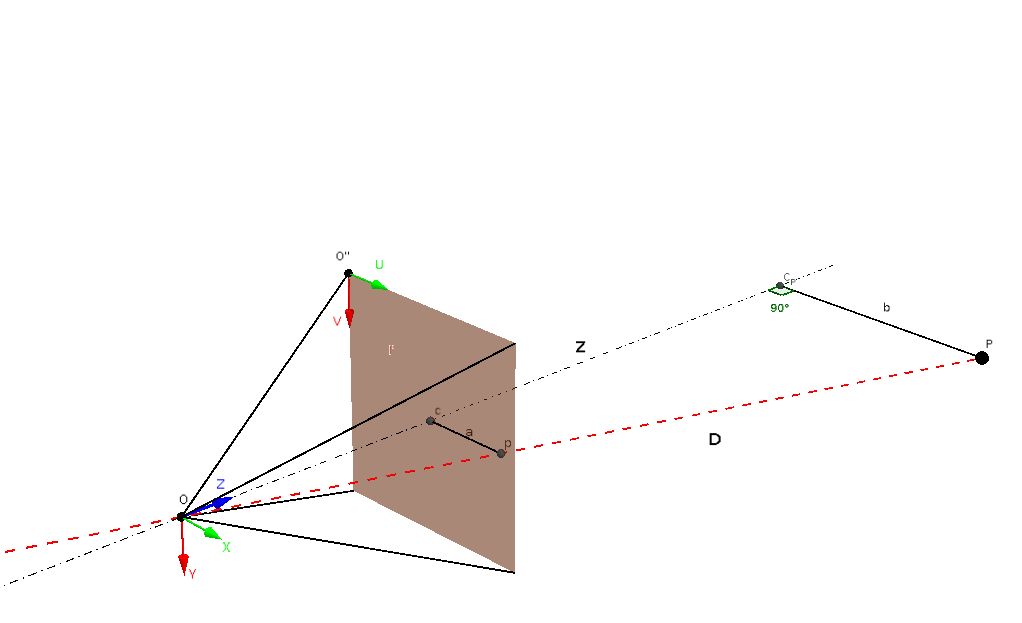
\includegraphics[width=12cm]{img/orf_depth.png}
		\caption{To compute the $(x_T,y_T,z_T)$ coordinates of the point $P$ given $(u_T,v_T)$ and $d_T$, we use the Pythagorean and Thales theorems}
		\label{fig:orf_depth}
	\end{center}
\end{figure}

In figure \ref{fig:orf_depth}, for each point $p_T^i$:
\begin{align}
x_T & =\dfrac{(u_T - c_U)}{z_T} f \tag{Pinhole model}\\
y_T & = \dfrac{(v_T - c_V)}{z_T} f \tag{Pinhole model}\\
\dfrac{f}{z_T} & = \dfrac{a}{b} \tag{Thales}\\
d^2 & = z_T^2 + b^2 \tag{Pythagoras}
\end{align}
Hence, after simplifications:
\begin{equation}
\begin{cases}
z_T = \sqrt{\dfrac{d_T^2}{1 + (u_T - c_U)^2 + \dfrac{(v_T - cV)^2}{f^2}}}\\\\
x_T = \dfrac{(u_T - c_U)}{z_T} f\\
y_T = \dfrac{(v_T - c_V)}{z_T} f
\end{cases}
\end{equation}

\subsubsection{Pose Estimation}
Now that the triangulation from the stereo cameras and the re-projection from the \gls{ORF} have been performed, we have a set of $i$ 3D points in two different coordinates systems $T$ and $L$ and we want to find the matrix $M_{LT}$ which minimizes the global errors between all those couple of points. The optimization problem can therefore be defined as:
\begin{equation}
M_{LT} = \mathtt{arg}\enspace \mathsf{min}\,\bigg\{\sum_{i=1}^n\, \lVert P_T^i - \hat{M}_{LT} * P_L^i \rVert^2\bigg\}
\end{equation}
This problem will be solve using Horn's absolute orientation algorithm \cite{absolute_orientation} into a Random Sample Consensus process (RANSAC) \cite{ransac}. Without going into further details, the idea behind Horn's algorithm is the following:
\begin{itemize*}
\item Compute the centroids for $L$ and $T$ points, find the translation between those centroids
\item Find the scale between the two points clouds
\item Rewrite the problem using quaternion so that the minimization can be reduced to finding eigenvalues of a matrix
\end{itemize*}
The RANSAC process aims at rejecting false positive measurement from the estimation scheme. For instance, if the checkerboard corner detection fails in one image and detect wrong points, we do not want those false positives to influence the total estimation. Intuitively, we know they can be spotted very quickly because the $M_{LT}$ they give is far from the $M_{LT}$ computed with all other points. We present the algorithm as summarized in \cite{muggler_phd}:

\begin{algorithm}
\caption{RANSAC: Random sample consensus}
\begin{algorithmic}[1]
\Function{RANSAC}{$data$, $max iterations$, $min inliers$}
\State $iteration \longleftarrow 0$;
\State $best model points \longleftarrow empty set$;
\While{$iterations < max iterations$ OR $best model points < min inliers$}
	\State $random points \longleftarrow$ select minimum number of $points$ randomly;
	\State $hypothesis model \longleftarrow$ estimate $model parameters$ using $random points$;
	\State $hypothesis points\, \longleftarrow\, random points$;
	\For{all $points$ except $random points$}
		\If{$point$ fits $hypothesis model$ with small error}
			\State Add $point$ to $hypothesis points$;
		\EndIf
	\EndFor
	\If{$hypothesis points$ has more $points$ than $best model points$}
		\State $best model points \longleftarrow  hypothesis points$;
	\EndIf
	\State $iterations \longleftarrow iterations + 1$;
\EndWhile
\State $best model \longleftarrow$ estimate model parameters using $best model points$;
\State Return $best model$;
\EndFunction
\end{algorithmic}
\end{algorithm}

\subsubsection{Extrinsic parameters computation}
In the end, we get the transformation matrix $M_{LT}$ and with the stereo extrinsic matrix $M_{LR}$, we can compute all extrinsic parameters:
\begin{equation}
M_{TL} = M_{LT}^{-1} \hspace{30pt} M_{RL} = M_{LR}^{-1} \hspace{30pt} M_{RT} = M_{RL} * M_{LT} \hspace{30pt} M_{TR} = M_{RT}^{-1}
\end{equation}

\newpage
\section{Fusion Algorithm}
\subsection{Literature Overview}
The goal of the fusion algorithm is to compute a 3D map of the environment, taking advantage of each sensor features in order to improve the global accuracy. Many articles have studied the realization of stereo and \gls{ToF} cameras fusion algorithm using various alternate methods. In order to understand more clearly, we can divide them into two categories:
\begin{itemize*}
\item In the first category, the stereo algorithm is performed alone without including the \gls{ToF} informations. As an output of this algorithm, we obtain a 3D map which can be compared to the \gls{ToF} 3D map to give a refined solution. This analyze is proposed in \cite{stereo_tof_fusion_realtime} where a final 3D map is deduced from the \gls{ToF} 3D map and the stereo 3D map by \textit{Winner takes it all} or \textit{Simulated annealing} strategies. According to their results, it gives real-time performances with a computation time lower than one second which is a true asset. In \cite{stereo_tof_fusion_patchlet}, 3D maps are fused along many patchlets areas using a \textit{Gauss-Markov Model}.
\item The second category implies incorporating the 3D information of the \gls{ToF} sensor directly in the stereo algorithm. Those methods seem to give good results but no information about the processing time is given. In \cite{stereo_tof_fusion_proba}, a full probability model is computed and an estimation maximizing the joint probability is then selected. The same kind of approach is used in \cite{stereo_tof_fusion_accuracy}. In \cite{stereo_tof_fusion}, the \gls{ToF} data are exploited in the initialization phase of a \textit{Dynamic Programming (DP)} algorithm developed in \cite{stereo_algorithm_KUL}. In another field of application, \cite{stereo_tof_fusion_3D_reconstruction} creates a joint probability of the two sensors to fulfill an occupancy grid and reconstruct a 3D object from multiple views.
\end{itemize*}
In this section, we will construct new algorithm based essentially on the work in \cite{stereo_tof_fusion_proba}.

\subsection{Overview}
\label{subsec:fusion:overview}

\subsubsection{Sensors}

% figure sensors
\begin{figure}[H] 
	\begin{center}
		{\scalefont{0.5}
		% Graphic for TeX using PGF
% Title: /home/gabs48/mit/thesis/graphic/sensors.dia
% Creator: Dia v0.97.2
% CreationDate: Fri Oct 10 15:03:48 2014
% For: gabs48
% \usepackage{tikz}
% The following commands are not supported in PSTricks at present
% We define them conditionally, so when they are implemented,
% this pgf file will use them.
\ifx\du\undefined
  \newlength{\du}
\fi
\setlength{\du}{15\unitlength}
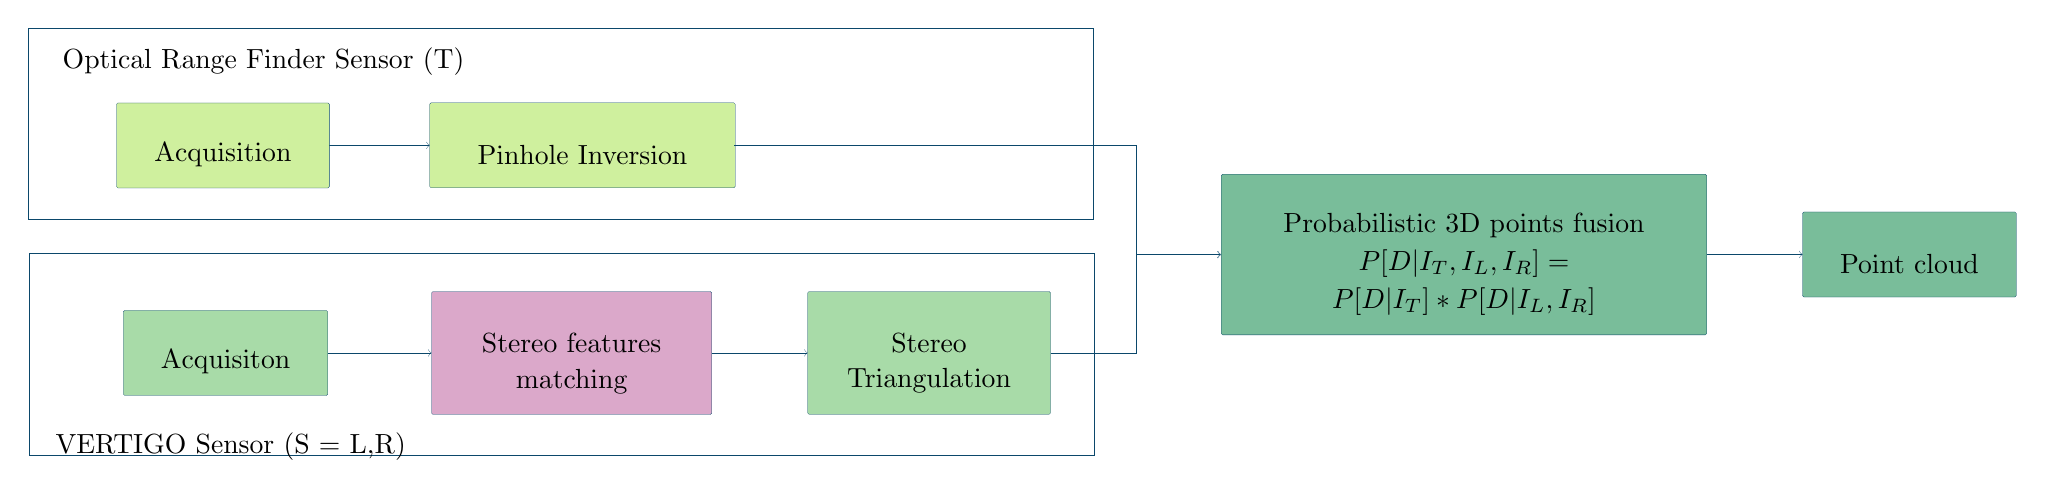
\begin{tikzpicture}
\pgftransformxscale{0.600000}
\pgftransformyscale{-0.600000}
\definecolor{dialinecolor}{rgb}{0.000000, 0.000000, 0.000000}
\pgfsetstrokecolor{dialinecolor}
\definecolor{dialinecolor}{rgb}{1.000000, 1.000000, 1.000000}
\pgfsetfillcolor{dialinecolor}
\pgfsetlinewidth{0.100000\du}
\pgfsetdash{}{0pt}
{\pgfsetcornersarced{\pgfpoint{0.500000\du}{0.500000\du}}\definecolor{dialinecolor}{rgb}{0.811765, 0.941176, 0.619608}
\pgfsetfillcolor{dialinecolor}
\fill (14.962113\du,11.000000\du)--(14.962113\du,12.800000\du)--(21.427113\du,12.800000\du)--(21.427113\du,11.000000\du)--cycle;
}{\pgfsetcornersarced{\pgfpoint{0.500000\du}{0.500000\du}}\definecolor{dialinecolor}{rgb}{0.043137, 0.282353, 0.419608}
\pgfsetstrokecolor{dialinecolor}
\draw (14.962113\du,11.000000\du)--(14.962113\du,12.800000\du)--(21.427113\du,12.800000\du)--(21.427113\du,11.000000\du)--cycle;
}% setfont left to latex
\definecolor{dialinecolor}{rgb}{0.043137, 0.282353, 0.419608}
\pgfsetstrokecolor{dialinecolor}
\node at (18.194613\du,12.095000\du){Pinhole Inversion};
\pgfsetlinewidth{0.100000\du}
\pgfsetdash{}{0pt}
{\pgfsetcornersarced{\pgfpoint{0.500000\du}{0.500000\du}}\definecolor{dialinecolor}{rgb}{0.858824, 0.658824, 0.792157}
\pgfsetfillcolor{dialinecolor}
\fill (15.000000\du,14.995264\du)--(15.000000\du,17.595264\du)--(20.932500\du,17.595264\du)--(20.932500\du,14.995264\du)--cycle;
}{\pgfsetcornersarced{\pgfpoint{0.500000\du}{0.500000\du}}\definecolor{dialinecolor}{rgb}{0.043137, 0.282353, 0.419608}
\pgfsetstrokecolor{dialinecolor}
\draw (15.000000\du,14.995264\du)--(15.000000\du,17.595264\du)--(20.932500\du,17.595264\du)--(20.932500\du,14.995264\du)--cycle;
}% setfont left to latex
\definecolor{dialinecolor}{rgb}{0.043137, 0.282353, 0.419608}
\pgfsetstrokecolor{dialinecolor}
\node at (17.966250\du,16.090264\du){Stereo features};
% setfont left to latex
\definecolor{dialinecolor}{rgb}{0.043137, 0.282353, 0.419608}
\pgfsetstrokecolor{dialinecolor}
\node at (17.966250\du,16.890264\du){ matching};
\pgfsetlinewidth{0.100000\du}
\pgfsetbuttcap
\pgfsetdash{}{0pt}
{
\definecolor{dialinecolor}{rgb}{0.043137, 0.282353, 0.419608}
\pgfsetfillcolor{dialinecolor}
% was here!!!
\pgfsetarrowsend{to}
\definecolor{dialinecolor}{rgb}{0.043137, 0.282353, 0.419608}
\pgfsetstrokecolor{dialinecolor}
\draw (12.837930\du,11.901712\du)--(13.900022\du,11.901712\du)--(13.900022\du,11.900000\du)--(14.962113\du,11.900000\du);
}
% setfont left to latex
\pgfsetlinewidth{0.100000\du}
\pgfsetbuttcap
\pgfsetdash{}{0pt}
{
\definecolor{dialinecolor}{rgb}{0.043137, 0.282353, 0.419608}
\pgfsetfillcolor{dialinecolor}
% was here!!!
\pgfsetarrowsend{to}
\definecolor{dialinecolor}{rgb}{0.043137, 0.282353, 0.419608}
\pgfsetstrokecolor{dialinecolor}
\draw (12.804756\du,16.294325\du)--(13.525000\du,16.294325\du)--(13.525000\du,16.295264\du)--(15.000000\du,16.295264\du);
}
% setfont left to latex
\pgfsetlinewidth{0.100000\du}
\pgfsetdash{}{0pt}
{\pgfsetcornersarced{\pgfpoint{0.500000\du}{0.500000\du}}\definecolor{dialinecolor}{rgb}{0.474510, 0.741176, 0.603922}
\pgfsetfillcolor{dialinecolor}
\fill (31.715151\du,12.511789\du)--(31.715151\du,15.911789\du)--(41.992651\du,15.911789\du)--(41.992651\du,12.511789\du)--cycle;
}{\pgfsetcornersarced{\pgfpoint{0.500000\du}{0.500000\du}}\definecolor{dialinecolor}{rgb}{0.043137, 0.282353, 0.419608}
\pgfsetstrokecolor{dialinecolor}
\draw (31.715151\du,12.511789\du)--(31.715151\du,15.911789\du)--(41.992651\du,15.911789\du)--(41.992651\du,12.511789\du)--cycle;
}% setfont left to latex
\definecolor{dialinecolor}{rgb}{0.043137, 0.282353, 0.419608}
\pgfsetstrokecolor{dialinecolor}
\node at (36.853901\du,13.606789\du){Probabilistic 3D points fusion};
% setfont left to latex
\definecolor{dialinecolor}{rgb}{0.043137, 0.282353, 0.419608}
\pgfsetstrokecolor{dialinecolor}
\node at (36.853901\du,14.406789\du){$P[D|I_T, I_L, I_R] =$};
% setfont left to latex
\definecolor{dialinecolor}{rgb}{0.043137, 0.282353, 0.419608}
\pgfsetstrokecolor{dialinecolor}
\node at (36.853901\du,15.206789\du){$P[D|I_T] * P[D|I_L,I_R]$};
\pgfsetlinewidth{0.100000\du}
\pgfsetdash{}{0pt}
{\pgfsetcornersarced{\pgfpoint{0.500000\du}{0.500000\du}}\definecolor{dialinecolor}{rgb}{0.658824, 0.858824, 0.658824}
\pgfsetfillcolor{dialinecolor}
\fill (22.961654\du,14.994000\du)--(22.961654\du,17.594000\du)--(28.101654\du,17.594000\du)--(28.101654\du,14.994000\du)--cycle;
}{\pgfsetcornersarced{\pgfpoint{0.500000\du}{0.500000\du}}\definecolor{dialinecolor}{rgb}{0.043137, 0.282353, 0.419608}
\pgfsetstrokecolor{dialinecolor}
\draw (22.961654\du,14.994000\du)--(22.961654\du,17.594000\du)--(28.101654\du,17.594000\du)--(28.101654\du,14.994000\du)--cycle;
}% setfont left to latex
\definecolor{dialinecolor}{rgb}{0.043137, 0.282353, 0.419608}
\pgfsetstrokecolor{dialinecolor}
\node at (25.531654\du,16.089000\du){Stereo};
% setfont left to latex
\definecolor{dialinecolor}{rgb}{0.043137, 0.282353, 0.419608}
\pgfsetstrokecolor{dialinecolor}
\node at (25.531654\du,16.889000\du){Triangulation};
\pgfsetlinewidth{0.100000\du}
\pgfsetdash{}{0pt}
{\pgfsetcornersarced{\pgfpoint{0.500000\du}{0.500000\du}}\definecolor{dialinecolor}{rgb}{0.811765, 0.941176, 0.619608}
\pgfsetfillcolor{dialinecolor}
\fill (8.332930\du,11.001712\du)--(8.332930\du,12.801712\du)--(12.837930\du,12.801712\du)--(12.837930\du,11.001712\du)--cycle;
}{\pgfsetcornersarced{\pgfpoint{0.500000\du}{0.500000\du}}\definecolor{dialinecolor}{rgb}{0.043137, 0.282353, 0.419608}
\pgfsetstrokecolor{dialinecolor}
\draw (8.332930\du,11.001712\du)--(8.332930\du,12.801712\du)--(12.837930\du,12.801712\du)--(12.837930\du,11.001712\du)--cycle;
}% setfont left to latex
\definecolor{dialinecolor}{rgb}{0.043137, 0.282353, 0.419608}
\pgfsetstrokecolor{dialinecolor}
\node at (10.585430\du,12.096712\du){Acquisition};
\pgfsetlinewidth{0.100000\du}
\pgfsetdash{}{0pt}
{\pgfsetcornersarced{\pgfpoint{0.500000\du}{0.500000\du}}\definecolor{dialinecolor}{rgb}{0.658824, 0.858824, 0.658824}
\pgfsetfillcolor{dialinecolor}
\fill (8.477256\du,15.394325\du)--(8.477256\du,17.194325\du)--(12.804756\du,17.194325\du)--(12.804756\du,15.394325\du)--cycle;
}{\pgfsetcornersarced{\pgfpoint{0.500000\du}{0.500000\du}}\definecolor{dialinecolor}{rgb}{0.043137, 0.282353, 0.419608}
\pgfsetstrokecolor{dialinecolor}
\draw (8.477256\du,15.394325\du)--(8.477256\du,17.194325\du)--(12.804756\du,17.194325\du)--(12.804756\du,15.394325\du)--cycle;
}% setfont left to latex
\definecolor{dialinecolor}{rgb}{0.043137, 0.282353, 0.419608}
\pgfsetstrokecolor{dialinecolor}
\node at (10.641006\du,16.489325\du){Acquisiton};
\pgfsetlinewidth{0.100000\du}
\pgfsetdash{}{0pt}
{\pgfsetcornersarced{\pgfpoint{0.500000\du}{0.500000\du}}\definecolor{dialinecolor}{rgb}{0.474510, 0.741176, 0.603922}
\pgfsetfillcolor{dialinecolor}
\fill (44.018906\du,13.310344\du)--(44.018906\du,15.110344\du)--(48.543906\du,15.110344\du)--(48.543906\du,13.310344\du)--cycle;
}{\pgfsetcornersarced{\pgfpoint{0.500000\du}{0.500000\du}}\definecolor{dialinecolor}{rgb}{0.043137, 0.282353, 0.419608}
\pgfsetstrokecolor{dialinecolor}
\draw (44.018906\du,13.310344\du)--(44.018906\du,15.110344\du)--(48.543906\du,15.110344\du)--(48.543906\du,13.310344\du)--cycle;
}% setfont left to latex
\definecolor{dialinecolor}{rgb}{0.043137, 0.282353, 0.419608}
\pgfsetstrokecolor{dialinecolor}
\node at (46.281406\du,14.405344\du){Point cloud};
\pgfsetlinewidth{0.100000\du}
\pgfsetbuttcap
\pgfsetdash{}{0pt}
{
\definecolor{dialinecolor}{rgb}{0.043137, 0.282353, 0.419608}
\pgfsetfillcolor{dialinecolor}
% was here!!!
\pgfsetarrowsend{to}
\definecolor{dialinecolor}{rgb}{0.043137, 0.282353, 0.419608}
\pgfsetstrokecolor{dialinecolor}
\draw (20.932500\du,16.295264\du)--(21.947077\du,16.295264\du)--(21.947077\du,16.294000\du)--(22.961654\du,16.294000\du);
}
% setfont left to latex
\pgfsetlinewidth{0.150000\du}
\pgfsetdash{}{0pt}
\pgfsetdash{}{0pt}
\pgfsetmiterjoin
\definecolor{dialinecolor}{rgb}{0.043137, 0.282353, 0.419608}
\pgfsetstrokecolor{dialinecolor}
\draw (6.456786\du,9.414155\du)--(6.456786\du,13.468052\du)--(28.999486\du,13.468052\du)--(28.999486\du,9.414155\du)--cycle;
\pgfsetlinewidth{0.150000\du}
\pgfsetdash{}{0pt}
\pgfsetdash{}{0pt}
\pgfsetmiterjoin
\definecolor{dialinecolor}{rgb}{0.043137, 0.282353, 0.419608}
\pgfsetstrokecolor{dialinecolor}
\draw (6.482533\du,14.183341\du)--(6.482533\du,18.469122\du)--(29.025233\du,18.469122\du)--(29.025233\du,14.183341\du)--cycle;
\pgfsetlinewidth{0.100000\du}
\pgfsetbuttcap
\pgfsetdash{}{0pt}
{
\definecolor{dialinecolor}{rgb}{0.043137, 0.282353, 0.419608}
\pgfsetfillcolor{dialinecolor}
% was here!!!
\pgfsetarrowsend{to}
\definecolor{dialinecolor}{rgb}{0.043137, 0.282353, 0.419608}
\pgfsetstrokecolor{dialinecolor}
\draw (21.412906\du,11.900000\du)--(29.904036\du,11.900000\du)--(29.904036\du,14.211789\du)--(31.700944\du,14.211789\du);
}
% setfont left to latex
\pgfsetlinewidth{0.100000\du}
\pgfsetbuttcap
\pgfsetdash{}{0pt}
{
\definecolor{dialinecolor}{rgb}{0.043137, 0.282353, 0.419608}
\pgfsetfillcolor{dialinecolor}
% was here!!!
\pgfsetarrowsend{to}
\definecolor{dialinecolor}{rgb}{0.043137, 0.282353, 0.419608}
\pgfsetstrokecolor{dialinecolor}
\draw (28.101654\du,16.294000\du)--(29.908403\du,16.294000\du)--(29.908403\du,14.211789\du)--(31.715151\du,14.211789\du);
}
% setfont left to latex
% setfont left to latex
\definecolor{dialinecolor}{rgb}{0.043137, 0.282353, 0.419608}
\pgfsetstrokecolor{dialinecolor}
\node[anchor=west] at (17.728136\du,11.441104\du){};
% setfont left to latex
\definecolor{dialinecolor}{rgb}{0.043137, 0.282353, 0.419608}
\pgfsetstrokecolor{dialinecolor}
\node[anchor=west] at (6.996674\du,10.124534\du){Optical Range Finder Sensor (T)};
% setfont left to latex
\definecolor{dialinecolor}{rgb}{0.043137, 0.282353, 0.419608}
\pgfsetstrokecolor{dialinecolor}
\node[anchor=west] at (6.845126\du,18.270216\du){VERTIGO Sensor (S = L,R)};
\pgfsetlinewidth{0.100000\du}
\pgfsetbuttcap
\pgfsetdash{}{0pt}
{
\definecolor{dialinecolor}{rgb}{0.043137, 0.282353, 0.419608}
\pgfsetfillcolor{dialinecolor}
% was here!!!
\pgfsetarrowsend{to}
\definecolor{dialinecolor}{rgb}{0.043137, 0.282353, 0.419608}
\pgfsetstrokecolor{dialinecolor}
\draw (41.992651\du,14.211789\du)--(43.005779\du,14.211789\du)--(43.005779\du,14.210344\du)--(44.018906\du,14.210344\du);
}
% setfont left to latex
\end{tikzpicture}

		}
	\end{center}
	\caption{The physical sensors of the \gls{INSPECT} project are represented with their software in a \textit{common representation format} which enables a probabilistic fusion \cite{multi_sensors_fusion}}\label{fig:sensors}
\end{figure}

If we adopt the representation and the notation in \cite{multi_sensors_fusion}, a \textit{sensor} $E$ is a system (hardware + software) characterized by its state, function, performances, output and energy type. In this case, we then consider two external sensors dedicated to navigation through 3D environment reconstruction whose output is a 3D point cloud combined with a monochromatic image (figure \ref{fig:sensors}). The performances are summarized in table \ref{table:perf}

\begin{center}
\begin{longtable}{|l|p{5.5cm}|p{5.5cm}|}
\hline
Performance & ORF & VERTIGO Sensors\\
\hline
Accuracy & Omnipresent noise & Good (if results)\\
\hline
Repeatability & Very good & Very good\\
\hline
Linearity & Non-linear with object speed and distance & Non-linear with object textures\\
\hline
Sensitivity & Sensible to luminous noise, saturation and movement & Sensible to the lack of texture in the environment\\
\hline
Resolution & Medium spatial resolution and good temporal resolution & Good spatial resolution and bad temporal resolution (computation)\\
\hline
Reliability & A result is guaranteed (but with variable quality) & Result not always guaranteed \\
\hline
Range & Very limited & Good\\
\hline
\caption{Performances of the two sensors according to the notation in \cite{multi_sensors_fusion}}\label{table:perf}
\end{longtable}
\end{center}

For each sensor, we can also define a \textit{sensor observation} $O$:
\begin{equation}
O = \langle E, \mathbf{x}, t, \mathbf{y}, \mathbf{\Delta y} \rangle
\end{equation}
Where:
\begin{itemize*}
\item $E$: the entity name which include the name of the physical property measured by the sensors as well as the units. Here, we measure \textit{3D point clouds} with their luminous intensity. In this work, we do not try to measure a spectral intensity as we will do next when the thermo-graphic camera will be added, we just need to know if the point exists or not (boolean measurement)
\item $\mathbf{x}$: the spatial location of the measurement (the 3D coordinates of each point in an absolute coordinate system)
\item $\mathbf{y}$: the value of the measurement (exists or not)
\item $\mathbf{\Delta y}$: a generic term which includes many types of errors including measurement, calibration, location,...
\end{itemize*}

\subsubsection{Fusion}
To perform fusion between them, the two \textit{sensors observations} must be represented in the same \textit{common representational format} which means we shall perform:
\begin{itemize*}
\item \textit{Spatial Alignment}: This process also called \textit{registration} consists of matching both sensors point clouds together. This task is one of the most important in the fusion and involves \textit{triangulation} and \textit{re-projection} using the calibration matrices as discussed in sections \ref{sec:stereo_camera} and \ref{sec:ORF_model}. In this work, we will do:
\begin{center}
2D points in $T$ reference system $\Rightarrow$ Triangulation $\Rightarrow$ 3D points in $T$ $\Rightarrow$ 3D points in $L$ $\Rightarrow$ Projection $\Rightarrow$ 2D points in $L$ and $R$
\end{center}
\item \textit{Temporal Alignment}: It is the transformation of the local times $t$ to a common time axis. In this work, we can estimate the image acquisition to be synchronous between the two devices (a system of time stamps has been implemented to guarantee this approximation) and we will not focus on this point.
\item \textit{Sensor Value Normalization}: As explained in \cite{multi_sensors_fusion}, normalizing two sensors with different physical properties is generally done by converting them into \textit{a posteriori probabilities}. In that case, estimated outputs are given by the application of the Bayes theorem. Here we can assimilate the computation of a 3D cloud to the research of a depth distribution $D$ which will be estimated by the system as a distribution $\hat{D}$ which maximizes the probability:
\begin{equation}
\hat{D} =  \mathtt{arg}\enspace \mathsf{max}\,\mathit{P}[D|I_T, I_L, I_R] =  \mathtt{arg}\enspace \mathsf{max}\,\dfrac{\mathit{P}[I_T, I_L, I_R|D] \mathit{P}[D]}{\mathit{P}[I_T, I_L, I_R]}
\end{equation}
Since $\mathit{P}[I_T, I_L, I_R]$ is not $D$-dependent, it can be replaced by any constant without changing the problem. Within those constants, let choose $\mathit{P}[I_T] \mathit{P}[I_L, I_R]$:
\begin{equation}
\hat{D} = \mathtt{arg}\enspace \mathsf{max}\,\dfrac{\mathit{P}[I_T, I_L, I_R|D] \mathit{P}[D]}{\mathit{P}[I_T] \mathit{P}[I_L, I_R]}
\end{equation}
As the camera depth distribution can be considered uniform, we can also write:
\begin{equation}
\hat{D} = \mathtt{arg}\enspace \mathsf{max}\,\dfrac{\mathit{P}[I_T, I_L, I_R|D] \mathit{P}[D]\mathit{P}[D]}{\mathit{P}[I_T] \mathit{P}[I_L, I_R]}
\end{equation}
One major hypothesis in the fusion is that $\{I_T, D\}$ and $\{I_L, I_R, D\}$ are independent \cite{stereo_tof_fusion_proba}. It leads to:
\begin{eqnarray}
\hat{D} & = & \mathtt{arg}\enspace \mathsf{max}\,\dfrac{\mathit{P}[I_T|D] \mathit{P}[D]}{\mathit{P}[I_T]}*\dfrac{\mathit{P}[I_L, I_R|D] \mathit{P}[D]}{\mathit{P}[I_L, I_R]}\\
\hat{D} & = & \mathtt{arg}\enspace \mathsf{max}\,\mathit{P}[D|I_T]*\mathit{P}[D|I_L, I_R]
\end{eqnarray}

\end{itemize*}
Finally, a fusion algorithm is characterized in terms of representation, certainty, accuracy, completeness. They will be discussed again when the results are introduced in chapter \ref{chapter:results} but we can already say:
\begin{itemize*}
\item \textbf{Representation}: This feature characterizing the abstraction level increasse from the algorithm inputs (2D matrices) to the algorithm outputs (3D point clouds).
\item \textbf{Certainty}: The gain in measurement certainty illustrates the growth between $\mathit{P}[D|I_T]$ and $\mathit{P}[D|I_L, I_R]$ on one hand and $\mathit{P}[D|I_T, I_L, I_R]$ on the other hand. It will be discussed in chapter \ref{chapter:results}.
\item \textbf{Accuracy}: The gain in measurement accuracy before and after the fusion will be discussed in chapter \ref{chapter:results}.
\item \textbf{Completeness}: The completeness will be affected by the limited \gls{FoV} of each cameras and the geometry between them. This feature is environment-dependent and will depend on the target size and distance and the application we want to perform.
\end{itemize*}

\subsection{Architecture}
All the concepts above leads to the architecture in figure \ref{fig:fusion_arch} that shows the big scheme of the fusion algorithm implemented in this thesis. However, there is a big difference compared to figure \ref{fig:sensors}. Indeed, we want to avoid \textit{feature matching} between stereo images which leads to bad results in poor textured environment. To avoid this problem, the fusion architecture in \cite{stereo_tof_fusion_proba} is exploited. This will be discussed in chapter \ref{chapter:results}.


\subsubsection{Determination of the Points Framed by all Cameras}
In order to perform \textit{registration}, the determination of the domain framed by both devices must be accomplished as the first step of the algorithm. We then only keep the points framed by the two cameras before proceeding to the fusion. Figure \ref{fig:geometry} shows the three devices \gls{FoV} in the $XZ$ plane. The hatched zone corresponds to the domain where fusion will take place. As we consider the three cameras have the same $Y$ coordinate, the $Y$ domain is given by the minimal \gls{FoV}. Basic analytical calculations give:
\begin{eqnarray}
z_i & \in & \Big[min\Big(\frac{t_{TR}\,\mathsf{tan}(\rho)\,\mathsf{tan}(\tau)}{\mathsf{tan}(\rho) + \mathsf{tan}(\tau)}, range_{min}\Big);\,range_{max}\Big]\\
x_i & \in & \Big[\dfrac{-z_i-t_{TR}\mathsf{tan}(\rho)}{\mathsf{tan}(\rho)};\,\dfrac{z_i}{\mathsf{tan}(\rho)}\Big]\\
y_i & \in & \Big[min\Big(\dfrac{-z_i}{\mathsf{tan}(\rho)}, \dfrac{-z_i}{\mathsf{tan}(\tau)}\Big);\,min\Big(\dfrac{z_i}{\mathsf{tan}(\rho)}, \dfrac{z_i}{\mathsf{tan}(\tau)}\Big)\Big]
\end{eqnarray}

% Figure geometry
\begin{figure}[!htt]
	\begin{center}
		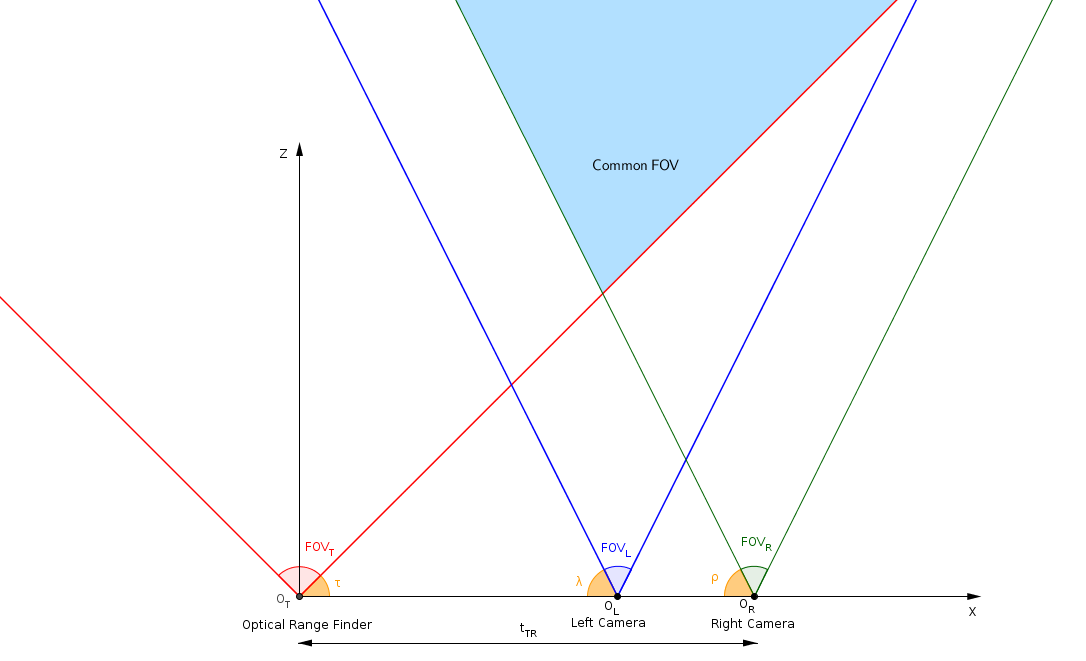
\includegraphics[width=10cm]{img/geometry.png}
		\caption{The region framed by the three cameras depends on the \textit{baseline} between the cameras as well as their \gls{FoV}}
		\label{fig:geometry}
	\end{center}
\end{figure}


\subsubsection{Optical Range Finder Noise Model}
According to \cite{orf_calib} and \cite{stereo_tof_fusion_proba}, the error in the depth measurement $\hat{D}_T$ for each pixel captured by the \gls{ORF} camera can be mainly described as the sum of the following components:
\begin{itemize*}
\item A \textit{thermal noise} with a Gaussian distribution
\item A \textit{quantization error}
\item A \textit{photon shot noise} with a Poisson distribution
\item A \textit{scattering generated noise} especially in presence of discontinuities
\end{itemize*}
According to the same sources, they consider the \textit{quantization error} and the \textit{photon shot noise} can be neglected in front of the \textit{thermal noise}. The latter can be represented by a Normal distribution around the measured depth:
\begin{equation}
\mathcal{N}(d_T^i, \sigma_t^2)
\end{equation}
Where $\sigma_t$ is inversely proportional to the confidence of the pixel given in the pixel map $C_T$. In our experiment set, we selected a factor $\sigma_t^2 = (range_{max} - C_T)/10$.
Concerning the scattering noise, \cite{orf_scattering} shows that it could also be expressed with a normal distribution:
\begin{equation}
\mathcal{N}(d_T^i, \sigma_s^2)
\end{equation}
Where $\sigma_s^2$ is the variance of the measured depths in the second order neighborhood of the considered pixel $p_T$.
Finally, the thermal noise is neglected near discontinuities and scattering noise far from discontinuities which gives:
\begin{equation}
\mathit{P}[d^i|I_T] \sim \mathcal{N}(d_T^i, \sigma_w^2)
\end{equation}
Where:
\begin{equation}
\sigma_w = \mathsf{max}(\sigma_t, \sigma_s)
\end{equation}

\subsubsection{Probabilistic Space Discretization}
Once the noise has been determined for each pixel, we can assume the real depth is situated at maximum $3 \sigma_w$ from the measured depth:
\begin{equation}
d^i \in [d_T^i - 3 \sigma_w;\,d_T^i + 3 \sigma_w]
\end{equation}

% figure orf_normal
\begin{figure}[H]
	\begin{center}
		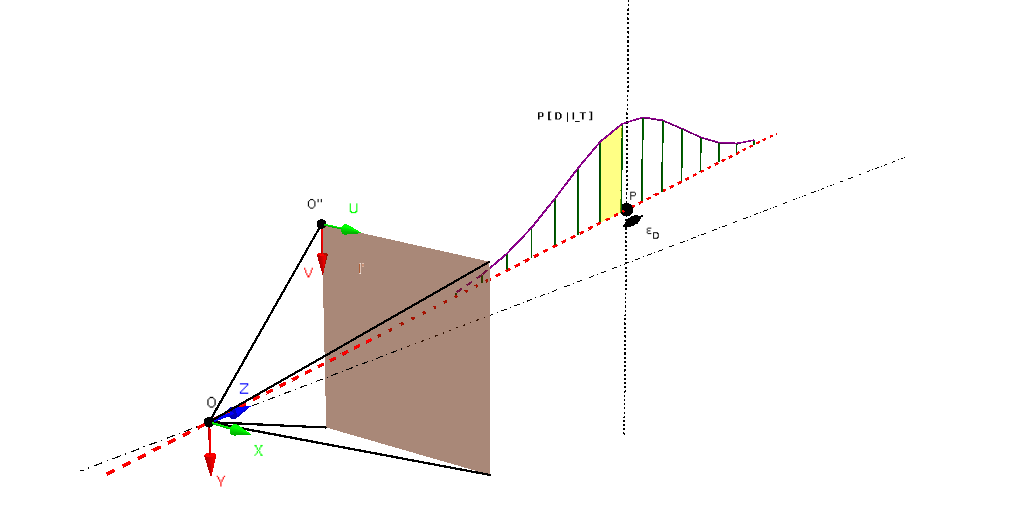
\includegraphics[width=12cm]{img/orf_normal.png}
		\caption{The interval around the measured depth $d_T^i$ is divided in $j$ steps of length $\epsilon_D$}
		\label{fig:orf_normal}
	\end{center}
\end{figure}


As presented in figure \ref{fig:orf_normal}, this interval is then discretized around $\hat{D}_T$ with a step equal to the stereoscopic accuracy sub-sampled by a factor $k_int$ ($k_{int} = 4$ in this work). In \cite{stereo_resolution} and \cite{stereo_resolution_2}, this resolution is equal to:
\begin{equation}
\label{eq:stereo_acc}
\epsilon_D = \dfrac{D^2}{b\, f}\,\epsilon_p
\end{equation}
Where $D$ is the depth, $b$ is the \textit{baseline} between $L$ and $R$ cameras, $f$ is the focal length (assumed to be the same for $L$ and $R$) and $\epsilon_p$ is the distance between two pixels on the camera ($6 \mu m$ for \gls{VERTIGO}) as shown in figure \ref{fig:cam_stereo_resolution}.

% figure cam_stereo_resolution
\begin{figure}[H]
	\begin{center}
		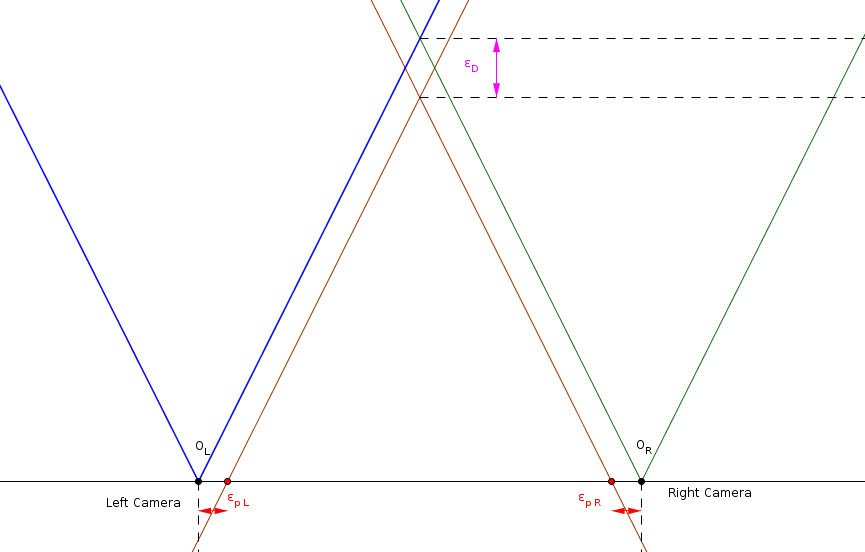
\includegraphics[width=6cm]{img/cam_stereo_resolution.png}
		\caption{The theoretical depth error for stereo devices depends on the depth $D$, the baseline between cameras $b$, the pixel size $\epsilon_p$ and the focal length $f$}
		\label{fig:cam_stereo_resolution}
	\end{center}
\end{figure}

\subsubsection{Optical Range Finder Probabilistic Model}
For each pixel of the depth map $d^i$ ($i=1..n$), we have constructed a sample of $j$ points $d^{i,j}$ ($j=1..m$) which are the candidates to represent the true depth $D$. As explained in section \ref{subsec:fusion:overview}, the next step to perform fusion consists of determining $\mathit{P}[d^i = d^{i,j} |I_T]$ and $\mathit{P}[d^i = d^{i,j}|I_L, I_R]$.
As shown previously, we can directly write:
\begin{equation}
\mathit{P}[d^i = d^{i,j}|I_T] = \frac{1}{\sigma_w^i \sqrt{2\pi} } e^{ -\frac{(d^{i,j} - d^i)^2}{2{\sigma_w^i}^2}}
\end{equation}

\subsubsection{Stereoscopic Cameras Probabilistic Model}
The computation of the probability $\mathit{P}[d^i = d^{i,j}|I_L, I_R]$ involves the re-projection of the 3D coordinates obtained for all $d^{i,j}$ from the \gls{ORF} (figure \ref{fig:stereo_proba}). It is a way to avoid straightforward feature matching whose results depend on the texture level of the scene as explained previously.

% Figure stereo_proba
\begin{figure}[H]
	\begin{center}
		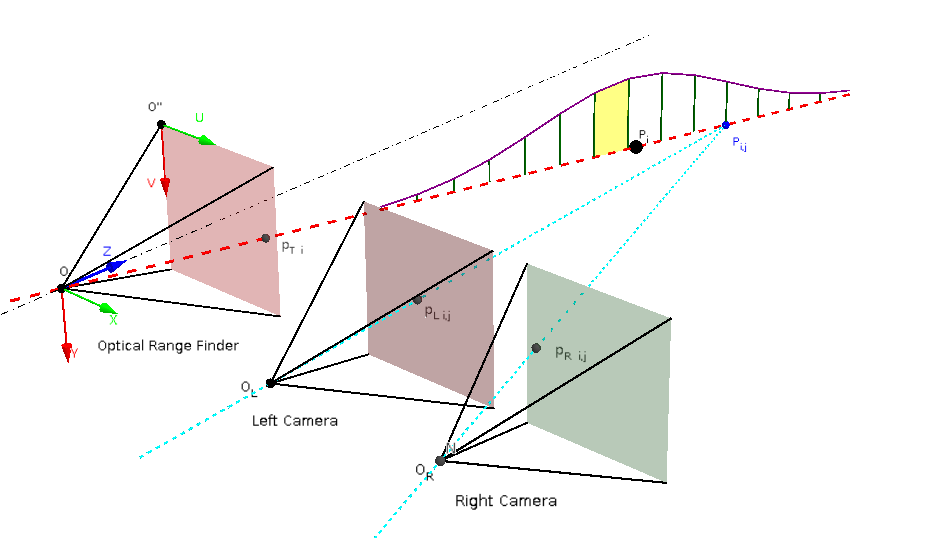
\includegraphics[width=12cm]{img/cam_stereo_proba.png}
		\caption{For each pixel, each $P_T^{i,j}$ is reprojected in $L$ and $R$ image planes. From those coordinates, a probability will be established to correct the depth measured by the \gls{ORF}}
		\label{fig:stereo_proba}
	\end{center}
\end{figure}

After this re-projection, the probability is computed as an exponential distribution which decreases according to a factor $c_{i,j}$ representing the degree of likeness between a point $P^{i,j}$ projected in $L$ and $R$:
\begin{equation}
\mathit{P}[d^i = d^{i,j}|I_L, I_R] = e^{\dfrac{-c_{i,j}}{\sigma_w^i}}
\end{equation}
In this way, when we project all the $j$ points discretized from the \gls{ORF} Normal probability of a pixel $i$, we can compute a degree likeness for each pair in $L$ and $R$. As a pixel is very tiny, a small offset could incur a big mismatch between $L$ and $R$ projection, that is why we consider a rectangular window of size $(k,l)$ around this point and we compute $c_{i,j}$ as a truncated sum of the absolute difference (\textit{L1-norm}) between each point of the window \cite{stereo_windowing}:
\begin{equation}
c_{i,j} = \mathsf{min}\Big\{\sum_k \sum_l\, \big|I_L(u_{i,j} + k, v_{i,j} + l) - I_R(u_{i,j} + k, v_{i,j} + l)\big|\,,\,thresh\Big\}
\end{equation}
Where the value $thresh$ will be discussed in the results.

\subsubsection{Joint Probability Computation}
For each pixel $i$, we deduce the joint probability:
\begin{equation}
\mathit{P}[d^i = d^{i,j}|I_T,I_L, I_R] = \mathit{P}[d^i = d^{i,j} |I_T]\,\,*\,\,\mathit{P}[d^i = d^{i,j}|I_L, I_R]
\end{equation}

\subsubsection{Depth Estimation Selection}
To create an improved 3D map, the last step consists of selecting the maximal probability in the selected interval for each pixel $i$:
\begin{equation}
\hat{d}_i = \mathsf{max}_{\,j} \Big\{\mathit{P}[d^i = d^{i,j}|I_T,I_L, I_R]\Big\}
\end{equation}

\subsubsection{3D Coordinates Computation}
From the variables $(u_T^i, v_T^i, \hat{d}_i)$, we recover $\hat{P}^i = (\hat{x}^i, \hat{y}^i, \hat{z}^i)$ by inverting the pinhole equation as described in \ref{subsubsec:orf_pinhole_inverstion}.

\subsubsection{Point Cloud Creation}
As a last step, a point cloud $\hat{\mathbf{P}}$ is composed by the assembly of every pixel $\hat{P}^i$

% Figure arch
\begin{figure}[!htt] 
	\begin{center}
		{\scalefont{0.5}
		% Graphic for TeX using PGF
% Title: /home/gabs48/mit/thesis/graphic/arch.dia
% Creator: Dia v0.97.2
% CreationDate: Fri Oct 10 17:15:52 2014
% For: gabs48
% \usepackage{tikz}
% The following commands are not supported in PSTricks at present
% We define them conditionally, so when they are implemented,
% this pgf file will use them.
\ifx\du\undefined
  \newlength{\du}
\fi
\setlength{\du}{15\unitlength}
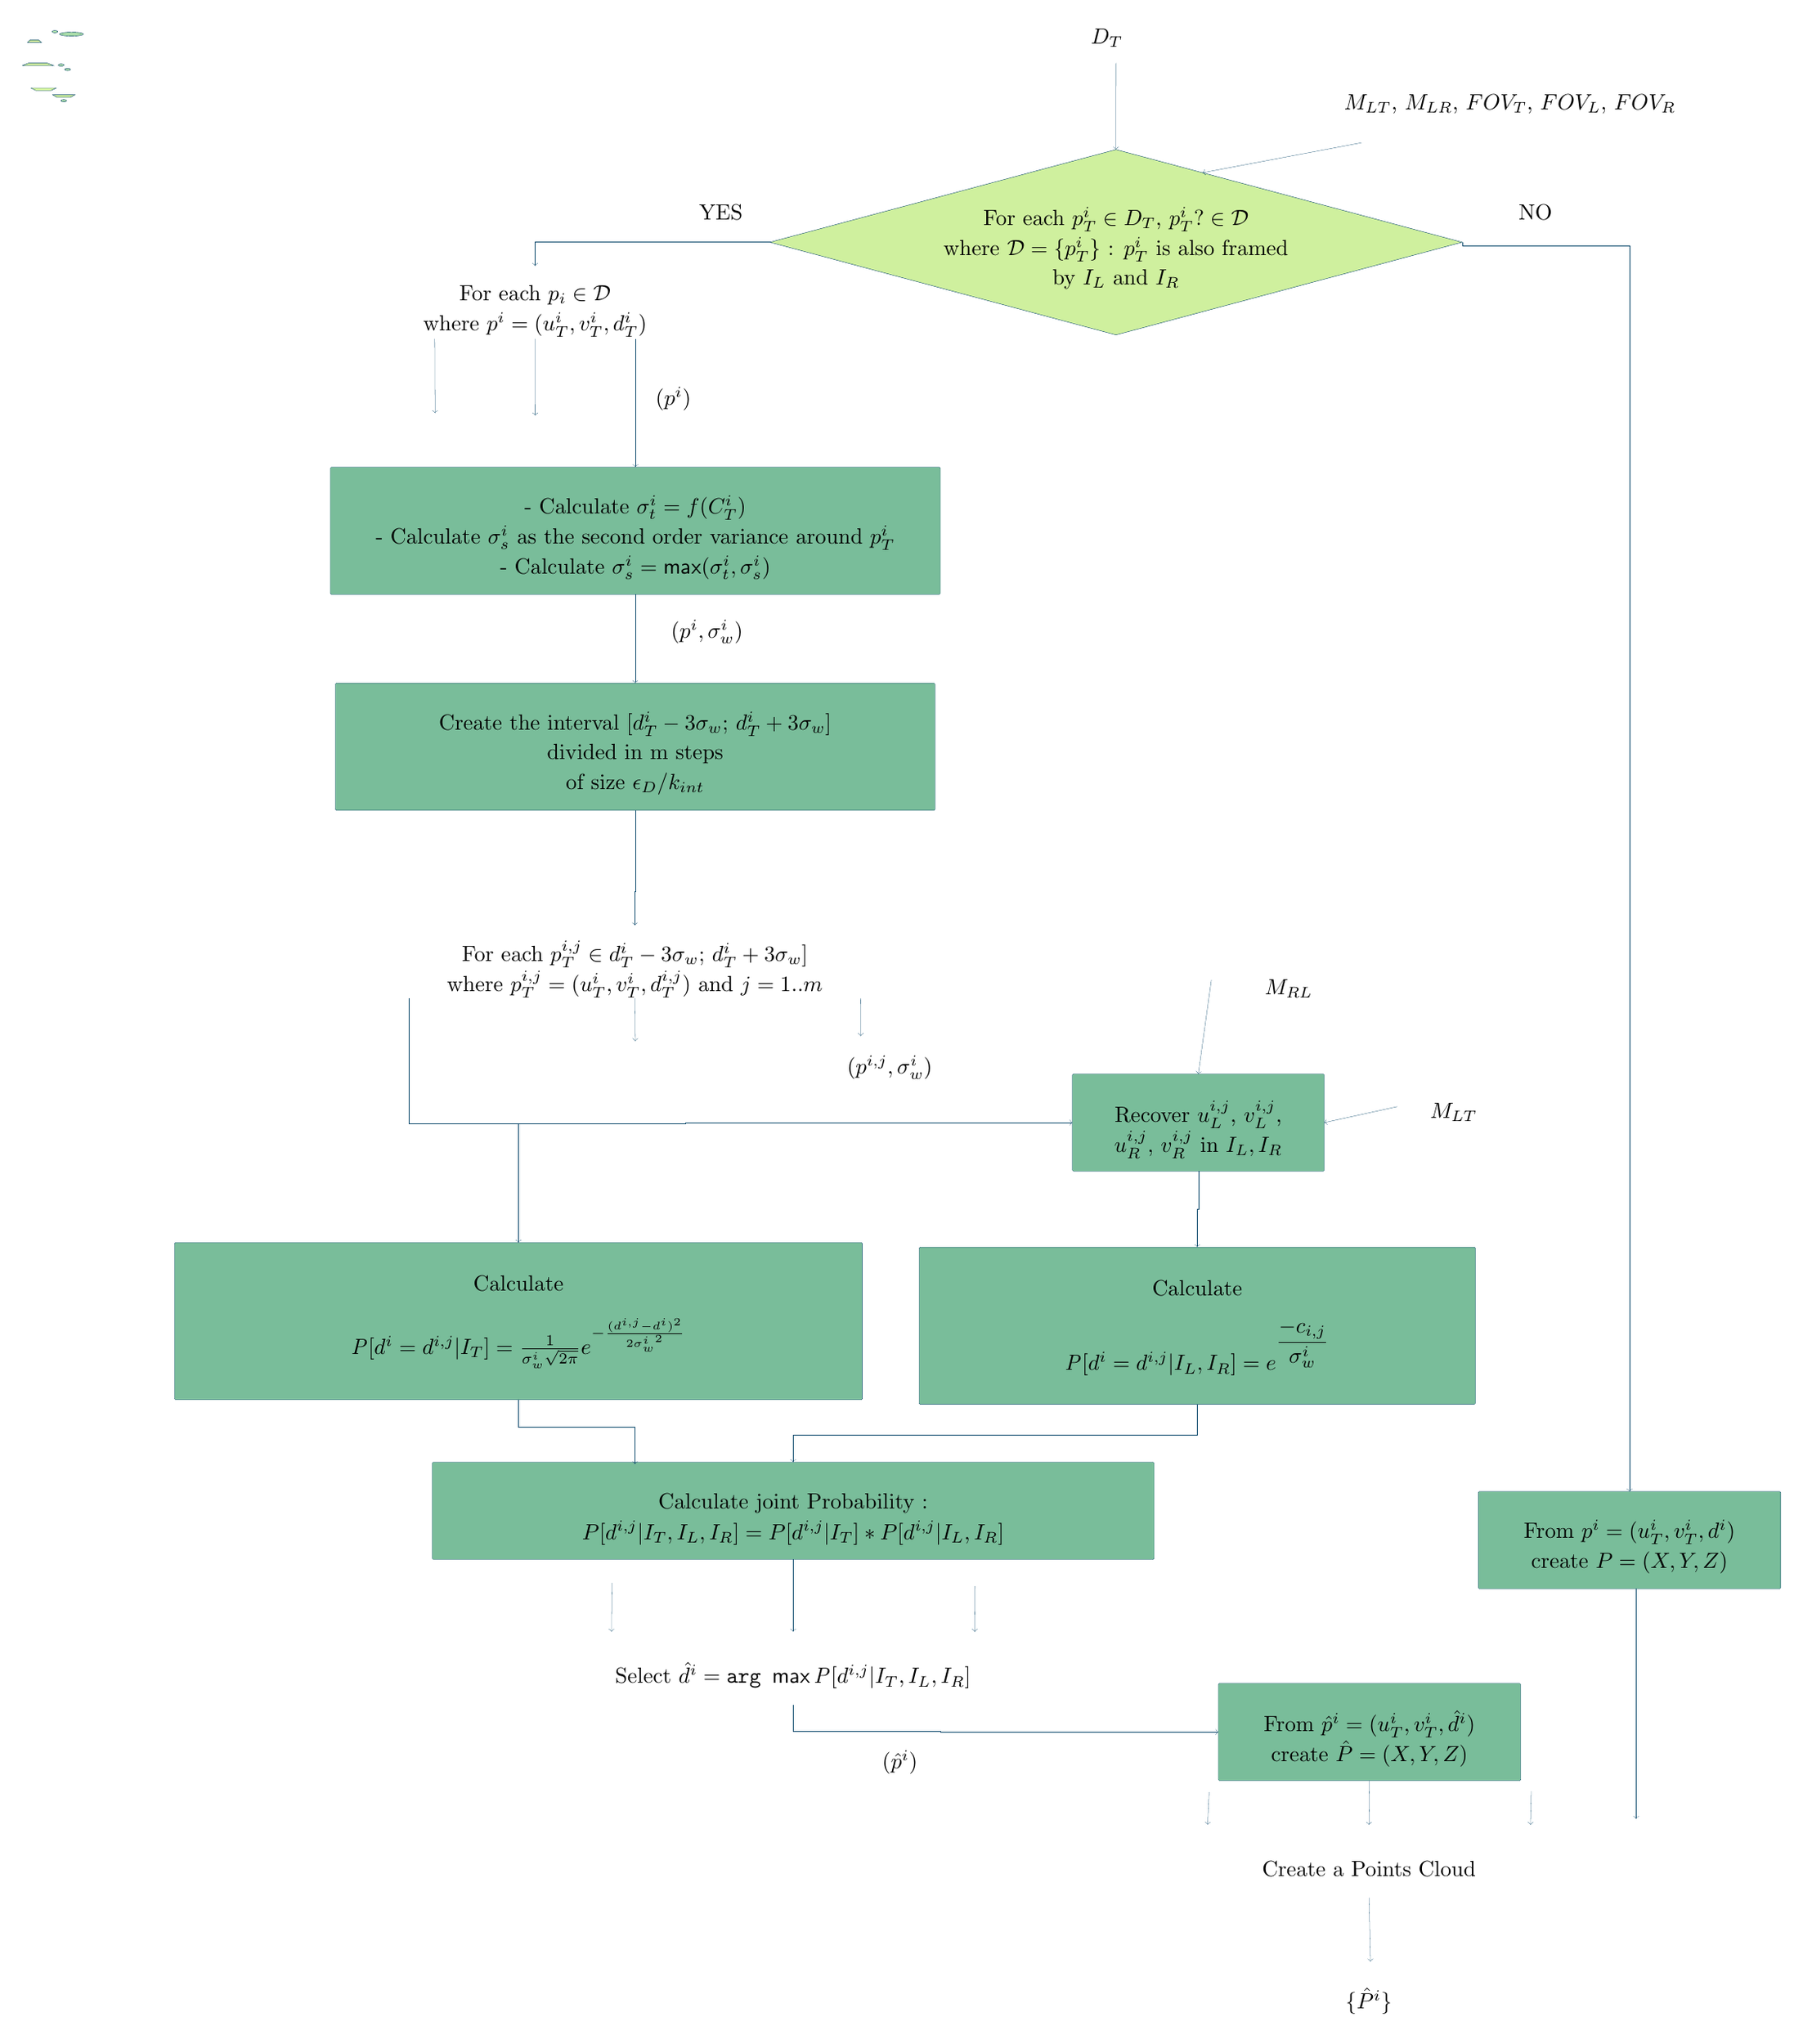
\begin{tikzpicture}
\pgftransformxscale{0.600000}
\pgftransformyscale{-0.600000}
\definecolor{dialinecolor}{rgb}{0.000000, 0.000000, 0.000000}
\pgfsetstrokecolor{dialinecolor}
\definecolor{dialinecolor}{rgb}{1.000000, 1.000000, 1.000000}
\pgfsetfillcolor{dialinecolor}
\pgfsetlinewidth{0.100000\du}
\pgfsetdash{}{0pt}
{\pgfsetcornersarced{\pgfpoint{0.500000\du}{0.500000\du}}\definecolor{dialinecolor}{rgb}{0.474510, 0.741176, 0.603922}
\pgfsetfillcolor{dialinecolor}
\fill (8.393256\du,11.632739\du)--(8.393256\du,15.032739\du)--(24.693256\du,15.032739\du)--(24.693256\du,11.632739\du)--cycle;
}{\pgfsetcornersarced{\pgfpoint{0.500000\du}{0.500000\du}}\definecolor{dialinecolor}{rgb}{0.043137, 0.282353, 0.419608}
\pgfsetstrokecolor{dialinecolor}
\draw (8.393256\du,11.632739\du)--(8.393256\du,15.032739\du)--(24.693256\du,15.032739\du)--(24.693256\du,11.632739\du)--cycle;
}% setfont left to latex
\definecolor{dialinecolor}{rgb}{0.043137, 0.282353, 0.419608}
\pgfsetstrokecolor{dialinecolor}
\node at (16.543256\du,12.727739\du){- Calculate $\sigma_t^i = f(C_T^i)$};
% setfont left to latex
\definecolor{dialinecolor}{rgb}{0.043137, 0.282353, 0.419608}
\pgfsetstrokecolor{dialinecolor}
\node at (16.543256\du,13.527739\du){- Calculate $\sigma_s^i$ as the second order variance around $p_T^{i}$};
% setfont left to latex
\definecolor{dialinecolor}{rgb}{0.043137, 0.282353, 0.419608}
\pgfsetstrokecolor{dialinecolor}
\node at (16.543256\du,14.327739\du){- Calculate $\sigma_s^i = \mathsf{max}(\sigma_t^i, \sigma_s^i)$};
\definecolor{dialinecolor}{rgb}{0.658824, 0.858824, 0.658824}
\pgfsetfillcolor{dialinecolor}
\pgfpathellipse{\pgfpoint{42.058077\du}{1.812780\du}}{\pgfpoint{9.090108\du}{0\du}}{\pgfpoint{0\du}{1.527626\du}}
\pgfusepath{fill}
\pgfsetlinewidth{0.150000\du}
\pgfsetdash{}{0pt}
\pgfsetdash{}{0pt}
\definecolor{dialinecolor}{rgb}{0.043137, 0.282353, 0.419608}
\pgfsetstrokecolor{dialinecolor}
\pgfpathellipse{\pgfpoint{42.058077\du}{1.812780\du}}{\pgfpoint{9.090108\du}{0\du}}{\pgfpoint{0\du}{1.527626\du}}
\pgfusepath{stroke}
\definecolor{dialinecolor}{rgb}{0.811765, 0.941176, 0.619608}
\pgfsetfillcolor{dialinecolor}
\fill (29.385659\du,3.147960\du)--(38.634070\du,5.623995\du)--(29.385659\du,8.100030\du)--(20.137247\du,5.623995\du)--cycle;
\pgfsetlinewidth{0.150000\du}
\pgfsetdash{}{0pt}
\pgfsetdash{}{0pt}
\pgfsetmiterjoin
\definecolor{dialinecolor}{rgb}{0.043137, 0.282353, 0.419608}
\pgfsetstrokecolor{dialinecolor}
\draw (29.385659\du,3.147960\du)--(38.634070\du,5.623995\du)--(29.385659\du,8.100030\du)--(20.137247\du,5.623995\du)--cycle;
% setfont left to latex
\definecolor{dialinecolor}{rgb}{0.043137, 0.282353, 0.419608}
\pgfsetstrokecolor{dialinecolor}
\node at (29.385659\du,5.018995\du){For each $p_T^i \in D_T$, $p_T^i ?\in \mathcal{D}$};
% setfont left to latex
\definecolor{dialinecolor}{rgb}{0.043137, 0.282353, 0.419608}
\pgfsetstrokecolor{dialinecolor}
\node at (29.385659\du,5.818995\du){where $\mathcal{D} = \{p_T^i\}$ : $p_T^i$ is also framed};
% setfont left to latex
\definecolor{dialinecolor}{rgb}{0.043137, 0.282353, 0.419608}
\pgfsetstrokecolor{dialinecolor}
\node at (29.385659\du,6.618995\du){by $I_L$ and $I_R$};
\definecolor{dialinecolor}{rgb}{0.658824, 0.858824, 0.658824}
\pgfsetfillcolor{dialinecolor}
\pgfpathellipse{\pgfpoint{29.387845\du}{-0.057395\du}}{\pgfpoint{2.216383\du}{0\du}}{\pgfpoint{0\du}{0.890342\du}}
\pgfusepath{fill}
\pgfsetlinewidth{0.150000\du}
\pgfsetdash{}{0pt}
\pgfsetdash{}{0pt}
\definecolor{dialinecolor}{rgb}{0.043137, 0.282353, 0.419608}
\pgfsetstrokecolor{dialinecolor}
\pgfpathellipse{\pgfpoint{29.387845\du}{-0.057395\du}}{\pgfpoint{2.216383\du}{0\du}}{\pgfpoint{0\du}{0.890342\du}}
\pgfusepath{stroke}
\pgfsetlinewidth{0.150000\du}
\pgfsetdash{}{0pt}
\pgfsetdash{}{0pt}
\pgfsetbuttcap
\pgfsetmiterjoin
\pgfsetlinewidth{0.150000\du}
\pgfsetbuttcap
\pgfsetmiterjoin
\pgfsetdash{}{0pt}
\definecolor{dialinecolor}{rgb}{0.811765, 0.941176, 0.619608}
\pgfsetfillcolor{dialinecolor}
\pgfpathmoveto{\pgfpoint{8.503452\du}{8.203952\du}}
\pgfpathlineto{\pgfpoint{19.225442\du}{8.203952\du}}
\pgfpathlineto{\pgfpoint{17.081044\du}{6.253952\du}}
\pgfpathlineto{\pgfpoint{10.647850\du}{6.253952\du}}
\pgfpathlineto{\pgfpoint{8.503452\du}{8.203952\du}}
\pgfusepath{fill}
\definecolor{dialinecolor}{rgb}{0.043137, 0.282353, 0.419608}
\pgfsetstrokecolor{dialinecolor}
\pgfpathmoveto{\pgfpoint{8.503452\du}{8.203952\du}}
\pgfpathlineto{\pgfpoint{19.225442\du}{8.203952\du}}
\pgfpathlineto{\pgfpoint{17.081044\du}{6.253952\du}}
\pgfpathlineto{\pgfpoint{10.647850\du}{6.253952\du}}
\pgfpathlineto{\pgfpoint{8.503452\du}{8.203952\du}}
\pgfusepath{stroke}
% setfont left to latex
\definecolor{dialinecolor}{rgb}{0.043137, 0.282353, 0.419608}
\pgfsetstrokecolor{dialinecolor}
\node at (13.864447\du,7.028952\du){For each $p_i \in \mathcal{D}$};
% setfont left to latex
\definecolor{dialinecolor}{rgb}{0.043137, 0.282353, 0.419608}
\pgfsetstrokecolor{dialinecolor}
\node at (13.864447\du,7.828952\du){where $p^i = (u_T^i, v_T^i, d_T^i)$};
\pgfsetlinewidth{0.100000\du}
\pgfsetdash{}{0pt}
{\pgfsetcornersarced{\pgfpoint{0.500000\du}{0.500000\du}}\definecolor{dialinecolor}{rgb}{0.474510, 0.741176, 0.603922}
\pgfsetfillcolor{dialinecolor}
\fill (8.527961\du,17.402406\du)--(8.527961\du,20.802406\du)--(24.550461\du,20.802406\du)--(24.550461\du,17.402406\du)--cycle;
}{\pgfsetcornersarced{\pgfpoint{0.500000\du}{0.500000\du}}\definecolor{dialinecolor}{rgb}{0.043137, 0.282353, 0.419608}
\pgfsetstrokecolor{dialinecolor}
\draw (8.527961\du,17.402406\du)--(8.527961\du,20.802406\du)--(24.550461\du,20.802406\du)--(24.550461\du,17.402406\du)--cycle;
}% setfont left to latex
\definecolor{dialinecolor}{rgb}{0.043137, 0.282353, 0.419608}
\pgfsetstrokecolor{dialinecolor}
\node at (16.539211\du,18.497406\du){Create the interval $[d_T^i - 3 \sigma_w;\,d_T^i + 3 \sigma_w]$};
% setfont left to latex
\definecolor{dialinecolor}{rgb}{0.043137, 0.282353, 0.419608}
\pgfsetstrokecolor{dialinecolor}
\node at (16.539211\du,19.297406\du){divided in m steps};
% setfont left to latex
\definecolor{dialinecolor}{rgb}{0.043137, 0.282353, 0.419608}
\pgfsetstrokecolor{dialinecolor}
\node at (16.539211\du,20.097406\du){of size $\epsilon_D/k_{int}$};
\pgfsetlinewidth{0.150000\du}
\pgfsetdash{}{0pt}
\pgfsetdash{}{0pt}
\pgfsetbuttcap
\pgfsetmiterjoin
\pgfsetlinewidth{0.150000\du}
\pgfsetbuttcap
\pgfsetmiterjoin
\pgfsetdash{}{0pt}
\definecolor{dialinecolor}{rgb}{0.811765, 0.941176, 0.619608}
\pgfsetfillcolor{dialinecolor}
\pgfpathmoveto{\pgfpoint{4.471471\du}{25.824234\du}}
\pgfpathlineto{\pgfpoint{28.590841\du}{25.824234\du}}
\pgfpathlineto{\pgfpoint{23.766967\du}{23.874234\du}}
\pgfpathlineto{\pgfpoint{9.295345\du}{23.874234\du}}
\pgfpathlineto{\pgfpoint{4.471471\du}{25.824234\du}}
\pgfusepath{fill}
\definecolor{dialinecolor}{rgb}{0.043137, 0.282353, 0.419608}
\pgfsetstrokecolor{dialinecolor}
\pgfpathmoveto{\pgfpoint{4.471471\du}{25.824234\du}}
\pgfpathlineto{\pgfpoint{28.590841\du}{25.824234\du}}
\pgfpathlineto{\pgfpoint{23.766967\du}{23.874234\du}}
\pgfpathlineto{\pgfpoint{9.295345\du}{23.874234\du}}
\pgfpathlineto{\pgfpoint{4.471471\du}{25.824234\du}}
\pgfusepath{stroke}
% setfont left to latex
\definecolor{dialinecolor}{rgb}{0.043137, 0.282353, 0.419608}
\pgfsetstrokecolor{dialinecolor}
\node at (16.531156\du,24.649234\du){For each $p_T^{i,j} \in d_T^i - 3 \sigma_w;\,d_T^i + 3 \sigma_w]$};
% setfont left to latex
\definecolor{dialinecolor}{rgb}{0.043137, 0.282353, 0.419608}
\pgfsetstrokecolor{dialinecolor}
\node at (16.531156\du,25.449234\du){where $p_T^{i,j} = (u_T^i, v_T^i, d_T^{i,j})$ and $j=1..m$};
\pgfsetlinewidth{0.100000\du}
\pgfsetdash{}{0pt}
{\pgfsetcornersarced{\pgfpoint{0.500000\du}{0.500000\du}}\definecolor{dialinecolor}{rgb}{0.474510, 0.741176, 0.603922}
\pgfsetfillcolor{dialinecolor}
\fill (4.228975\du,32.349730\du)--(4.228975\du,36.549730\du)--(22.608975\du,36.549730\du)--(22.608975\du,32.349730\du)--cycle;
}{\pgfsetcornersarced{\pgfpoint{0.500000\du}{0.500000\du}}\definecolor{dialinecolor}{rgb}{0.043137, 0.282353, 0.419608}
\pgfsetstrokecolor{dialinecolor}
\draw (4.228975\du,32.349730\du)--(4.228975\du,36.549730\du)--(22.608975\du,36.549730\du)--(22.608975\du,32.349730\du)--cycle;
}% setfont left to latex
\definecolor{dialinecolor}{rgb}{0.043137, 0.282353, 0.419608}
\pgfsetstrokecolor{dialinecolor}
\node at (13.418975\du,33.444730\du){Calculate};
% setfont left to latex
\definecolor{dialinecolor}{rgb}{0.043137, 0.282353, 0.419608}
\pgfsetstrokecolor{dialinecolor}
\node at (13.418975\du,34.244730\du){};
% setfont left to latex
\definecolor{dialinecolor}{rgb}{0.043137, 0.282353, 0.419608}
\pgfsetstrokecolor{dialinecolor}
\node at (13.418975\du,35.044730\du){$\mathit{P}[d^i = d^{i,j}|I_T] = \frac{1}{\sigma_w^i \sqrt{2\pi} } e^{ -\frac{(d^{i,j} - d^i)^2}{2{\sigma_w^i}^2}}$};
% setfont left to latex
\definecolor{dialinecolor}{rgb}{0.043137, 0.282353, 0.419608}
\pgfsetstrokecolor{dialinecolor}
\node at (13.418975\du,35.844730\du){};
\pgfsetlinewidth{0.100000\du}
\pgfsetdash{}{0pt}
{\pgfsetcornersarced{\pgfpoint{0.500000\du}{0.500000\du}}\definecolor{dialinecolor}{rgb}{0.474510, 0.741176, 0.603922}
\pgfsetfillcolor{dialinecolor}
\fill (28.220357\du,27.844371\du)--(28.220357\du,30.444371\du)--(34.950357\du,30.444371\du)--(34.950357\du,27.844371\du)--cycle;
}{\pgfsetcornersarced{\pgfpoint{0.500000\du}{0.500000\du}}\definecolor{dialinecolor}{rgb}{0.043137, 0.282353, 0.419608}
\pgfsetstrokecolor{dialinecolor}
\draw (28.220357\du,27.844371\du)--(28.220357\du,30.444371\du)--(34.950357\du,30.444371\du)--(34.950357\du,27.844371\du)--cycle;
}% setfont left to latex
\definecolor{dialinecolor}{rgb}{0.043137, 0.282353, 0.419608}
\pgfsetstrokecolor{dialinecolor}
\node at (31.585357\du,28.939371\du){Recover $u_L^{i,j}$, $v_L^{i,j}$,};
% setfont left to latex
\definecolor{dialinecolor}{rgb}{0.043137, 0.282353, 0.419608}
\pgfsetstrokecolor{dialinecolor}
\node at (31.585357\du,29.739371\du){$u_R^{i,j}$, $v_R^{i,j}$ in $I_L, I_R$};
\pgfsetlinewidth{0.100000\du}
\pgfsetdash{}{0pt}
{\pgfsetcornersarced{\pgfpoint{0.500000\du}{0.500000\du}}\definecolor{dialinecolor}{rgb}{0.474510, 0.741176, 0.603922}
\pgfsetfillcolor{dialinecolor}
\fill (24.126652\du,32.471767\du)--(24.126652\du,36.671767\du)--(38.989152\du,36.671767\du)--(38.989152\du,32.471767\du)--cycle;
}{\pgfsetcornersarced{\pgfpoint{0.500000\du}{0.500000\du}}\definecolor{dialinecolor}{rgb}{0.043137, 0.282353, 0.419608}
\pgfsetstrokecolor{dialinecolor}
\draw (24.126652\du,32.471767\du)--(24.126652\du,36.671767\du)--(38.989152\du,36.671767\du)--(38.989152\du,32.471767\du)--cycle;
}% setfont left to latex
\definecolor{dialinecolor}{rgb}{0.043137, 0.282353, 0.419608}
\pgfsetstrokecolor{dialinecolor}
\node at (31.557902\du,33.566767\du){Calculate};
% setfont left to latex
\definecolor{dialinecolor}{rgb}{0.043137, 0.282353, 0.419608}
\pgfsetstrokecolor{dialinecolor}
\node at (31.557902\du,34.366767\du){};
% setfont left to latex
\definecolor{dialinecolor}{rgb}{0.043137, 0.282353, 0.419608}
\pgfsetstrokecolor{dialinecolor}
\node at (31.557902\du,35.166767\du){$\mathit{P}[d^i = d^{i,j}|I_L, I_R] = e^{\dfrac{-c_{i,j}}{\sigma_w^i}}$};
% setfont left to latex
\definecolor{dialinecolor}{rgb}{0.043137, 0.282353, 0.419608}
\pgfsetstrokecolor{dialinecolor}
\node at (31.557902\du,35.966767\du){};
\pgfsetlinewidth{0.100000\du}
\pgfsetdash{}{0pt}
{\pgfsetcornersarced{\pgfpoint{0.500000\du}{0.500000\du}}\definecolor{dialinecolor}{rgb}{0.474510, 0.741176, 0.603922}
\pgfsetfillcolor{dialinecolor}
\fill (11.114189\du,38.215757\du)--(11.114189\du,40.815757\du)--(30.404189\du,40.815757\du)--(30.404189\du,38.215757\du)--cycle;
}{\pgfsetcornersarced{\pgfpoint{0.500000\du}{0.500000\du}}\definecolor{dialinecolor}{rgb}{0.043137, 0.282353, 0.419608}
\pgfsetstrokecolor{dialinecolor}
\draw (11.114189\du,38.215757\du)--(11.114189\du,40.815757\du)--(30.404189\du,40.815757\du)--(30.404189\du,38.215757\du)--cycle;
}% setfont left to latex
\definecolor{dialinecolor}{rgb}{0.043137, 0.282353, 0.419608}
\pgfsetstrokecolor{dialinecolor}
\node at (20.759189\du,39.310757\du){Calculate joint Probability :};
% setfont left to latex
\definecolor{dialinecolor}{rgb}{0.043137, 0.282353, 0.419608}
\pgfsetstrokecolor{dialinecolor}
\node at (20.759189\du,40.110757\du){                                              $P[d^{i,j}|I_T, I_L, I_R] = P[d^{i,j}|I_T] * P[d^{i,j}|I_L,I_R]$};
\pgfsetlinewidth{0.150000\du}
\pgfsetdash{}{0pt}
\pgfsetdash{}{0pt}
\pgfsetbuttcap
\pgfsetmiterjoin
\pgfsetlinewidth{0.150000\du}
\pgfsetbuttcap
\pgfsetmiterjoin
\pgfsetdash{}{0pt}
\definecolor{dialinecolor}{rgb}{0.811765, 0.941176, 0.619608}
\pgfsetfillcolor{dialinecolor}
\pgfpathmoveto{\pgfpoint{11.051951\du}{42.746384\du}}
\pgfpathlineto{\pgfpoint{30.463785\du}{42.746384\du}}
\pgfpathlineto{\pgfpoint{26.581418\du}{44.696384\du}}
\pgfpathlineto{\pgfpoint{14.934318\du}{44.696384\du}}
\pgfpathlineto{\pgfpoint{11.051951\du}{42.746384\du}}
\pgfusepath{fill}
\definecolor{dialinecolor}{rgb}{0.043137, 0.282353, 0.419608}
\pgfsetstrokecolor{dialinecolor}
\pgfpathmoveto{\pgfpoint{11.051951\du}{42.746384\du}}
\pgfpathlineto{\pgfpoint{30.463785\du}{42.746384\du}}
\pgfpathlineto{\pgfpoint{26.581418\du}{44.696384\du}}
\pgfpathlineto{\pgfpoint{14.934318\du}{44.696384\du}}
\pgfpathlineto{\pgfpoint{11.051951\du}{42.746384\du}}
\pgfusepath{stroke}
% setfont left to latex
\definecolor{dialinecolor}{rgb}{0.043137, 0.282353, 0.419608}
\pgfsetstrokecolor{dialinecolor}
\node at (20.757868\du,43.921384\du){Select $\hat{d}^i = \mathtt{arg}\enspace \mathsf{max}\,\mathit{P}[d^{i,j}|I_T, I_L, I_R]$};
\definecolor{dialinecolor}{rgb}{0.658824, 0.858824, 0.658824}
\pgfsetfillcolor{dialinecolor}
\pgfpathellipse{\pgfpoint{34.149677\du}{25.334284\du}}{\pgfpoint{2.216383\du}{0\du}}{\pgfpoint{0\du}{0.890342\du}}
\pgfusepath{fill}
\pgfsetlinewidth{0.150000\du}
\pgfsetdash{}{0pt}
\pgfsetdash{}{0pt}
\definecolor{dialinecolor}{rgb}{0.043137, 0.282353, 0.419608}
\pgfsetstrokecolor{dialinecolor}
\pgfpathellipse{\pgfpoint{34.149677\du}{25.334284\du}}{\pgfpoint{2.216383\du}{0\du}}{\pgfpoint{0\du}{0.890342\du}}
\pgfusepath{stroke}
\definecolor{dialinecolor}{rgb}{0.658824, 0.858824, 0.658824}
\pgfsetfillcolor{dialinecolor}
\pgfpathellipse{\pgfpoint{39.116990\du}{28.717865\du}}{\pgfpoint{2.216383\du}{0\du}}{\pgfpoint{0\du}{0.890342\du}}
\pgfusepath{fill}
\pgfsetlinewidth{0.150000\du}
\pgfsetdash{}{0pt}
\pgfsetdash{}{0pt}
\definecolor{dialinecolor}{rgb}{0.043137, 0.282353, 0.419608}
\pgfsetstrokecolor{dialinecolor}
\pgfpathellipse{\pgfpoint{39.116990\du}{28.717865\du}}{\pgfpoint{2.216383\du}{0\du}}{\pgfpoint{0\du}{0.890342\du}}
\pgfusepath{stroke}
\pgfsetlinewidth{0.150000\du}
\pgfsetdash{}{0pt}
\pgfsetdash{}{0pt}
\pgfsetbuttcap
\pgfsetmiterjoin
\pgfsetlinewidth{0.150000\du}
\pgfsetbuttcap
\pgfsetmiterjoin
\pgfsetdash{}{0pt}
\definecolor{dialinecolor}{rgb}{0.811765, 0.941176, 0.619608}
\pgfsetfillcolor{dialinecolor}
\pgfpathmoveto{\pgfpoint{27.521062\du}{47.902946\du}}
\pgfpathlineto{\pgfpoint{44.771062\du}{47.902946\du}}
\pgfpathlineto{\pgfpoint{41.321062\du}{49.852946\du}}
\pgfpathlineto{\pgfpoint{30.971062\du}{49.852946\du}}
\pgfpathlineto{\pgfpoint{27.521062\du}{47.902946\du}}
\pgfusepath{fill}
\definecolor{dialinecolor}{rgb}{0.043137, 0.282353, 0.419608}
\pgfsetstrokecolor{dialinecolor}
\pgfpathmoveto{\pgfpoint{27.521062\du}{47.902946\du}}
\pgfpathlineto{\pgfpoint{44.771062\du}{47.902946\du}}
\pgfpathlineto{\pgfpoint{41.321062\du}{49.852946\du}}
\pgfpathlineto{\pgfpoint{30.971062\du}{49.852946\du}}
\pgfpathlineto{\pgfpoint{27.521062\du}{47.902946\du}}
\pgfusepath{stroke}
% setfont left to latex
\definecolor{dialinecolor}{rgb}{0.043137, 0.282353, 0.419608}
\pgfsetstrokecolor{dialinecolor}
\node at (36.146062\du,49.077946\du){Create a Points Cloud};
\pgfsetlinewidth{0.100000\du}
\pgfsetdash{}{0pt}
{\pgfsetcornersarced{\pgfpoint{0.500000\du}{0.500000\du}}\definecolor{dialinecolor}{rgb}{0.474510, 0.741176, 0.603922}
\pgfsetfillcolor{dialinecolor}
\fill (32.118851\du,44.125315\du)--(32.118851\du,46.725315\du)--(40.198851\du,46.725315\du)--(40.198851\du,44.125315\du)--cycle;
}{\pgfsetcornersarced{\pgfpoint{0.500000\du}{0.500000\du}}\definecolor{dialinecolor}{rgb}{0.043137, 0.282353, 0.419608}
\pgfsetstrokecolor{dialinecolor}
\draw (32.118851\du,44.125315\du)--(32.118851\du,46.725315\du)--(40.198851\du,46.725315\du)--(40.198851\du,44.125315\du)--cycle;
}% setfont left to latex
\definecolor{dialinecolor}{rgb}{0.043137, 0.282353, 0.419608}
\pgfsetstrokecolor{dialinecolor}
\node at (36.158851\du,45.220315\du){From $\hat{p}^i = (u_T^i, v_T^i, \hat{d}^i)$};
% setfont left to latex
\definecolor{dialinecolor}{rgb}{0.043137, 0.282353, 0.419608}
\pgfsetstrokecolor{dialinecolor}
\node at (36.158851\du,46.020315\du){create $\hat{P} = (X,Y,Z)$};
\definecolor{dialinecolor}{rgb}{0.658824, 0.858824, 0.658824}
\pgfsetfillcolor{dialinecolor}
\pgfpathellipse{\pgfpoint{36.185651\du}{52.447506\du}}{\pgfpoint{2.216383\du}{0\du}}{\pgfpoint{0\du}{0.890342\du}}
\pgfusepath{fill}
\pgfsetlinewidth{0.150000\du}
\pgfsetdash{}{0pt}
\pgfsetdash{}{0pt}
\definecolor{dialinecolor}{rgb}{0.043137, 0.282353, 0.419608}
\pgfsetstrokecolor{dialinecolor}
\pgfpathellipse{\pgfpoint{36.185651\du}{52.447506\du}}{\pgfpoint{2.216383\du}{0\du}}{\pgfpoint{0\du}{0.890342\du}}
\pgfusepath{stroke}
\pgfsetlinewidth{0.100000\du}
\pgfsetbuttcap
\pgfsetdash{}{0pt}
{
\definecolor{dialinecolor}{rgb}{0.043137, 0.282353, 0.419608}
\pgfsetfillcolor{dialinecolor}
% was here!!!
\pgfsetarrowsend{to}
\definecolor{dialinecolor}{rgb}{0.043137, 0.282353, 0.419608}
\pgfsetstrokecolor{dialinecolor}
\draw (20.137247\du,5.623995\du)--(20.137247\du,5.617463\du)--(13.864447\du,5.617463\du)--(13.864447\du,6.253952\du);
}
% setfont left to latex
\pgfsetlinewidth{0.100000\du}
\pgfsetbuttcap
\pgfsetdash{}{0pt}
{
\definecolor{dialinecolor}{rgb}{0.043137, 0.282353, 0.419608}
\pgfsetfillcolor{dialinecolor}
% was here!!!
\pgfsetarrowsend{to}
\definecolor{dialinecolor}{rgb}{0.043137, 0.282353, 0.419608}
\pgfsetstrokecolor{dialinecolor}
\draw (16.544944\du,8.203952\du)--(16.544944\du,9.646562\du)--(16.541954\du,9.646562\du)--(16.541954\du,10.132739\du)--(16.543256\du,10.132739\du)--(16.543256\du,11.632739\du);
}
% setfont left to latex
\pgfsetlinewidth{0.100000\du}
\pgfsetbuttcap
\pgfsetdash{}{0pt}
{
\definecolor{dialinecolor}{rgb}{0.043137, 0.282353, 0.419608}
\pgfsetfillcolor{dialinecolor}
% was here!!!
\pgfsetarrowsend{to}
\definecolor{dialinecolor}{rgb}{0.043137, 0.282353, 0.419608}
\pgfsetstrokecolor{dialinecolor}
\draw (16.543256\du,15.032739\du)--(16.543256\du,16.217573\du)--(16.539211\du,16.217573\du)--(16.539211\du,17.402406\du);
}
% setfont left to latex
\pgfsetlinewidth{0.100000\du}
\pgfsetbuttcap
\pgfsetdash{}{0pt}
{
\definecolor{dialinecolor}{rgb}{0.043137, 0.282353, 0.419608}
\pgfsetfillcolor{dialinecolor}
% was here!!!
\pgfsetarrowsend{to}
\definecolor{dialinecolor}{rgb}{0.043137, 0.282353, 0.419608}
\pgfsetstrokecolor{dialinecolor}
\draw (16.539211\du,20.802406\du)--(16.539211\du,22.294875\du)--(16.541575\du,22.294875\du)--(16.541575\du,22.969630\du)--(16.531156\du,22.969630\du)--(16.531156\du,23.874234\du);
}
% setfont left to latex
\pgfsetlinewidth{0.100000\du}
\pgfsetbuttcap
\pgfsetdash{}{0pt}
{
\definecolor{dialinecolor}{rgb}{0.043137, 0.282353, 0.419608}
\pgfsetfillcolor{dialinecolor}
% was here!!!
\pgfsetarrowsend{to}
\definecolor{dialinecolor}{rgb}{0.043137, 0.282353, 0.419608}
\pgfsetstrokecolor{dialinecolor}
\draw (31.585357\du,30.444371\du)--(31.585357\du,31.458069\du)--(31.557902\du,31.458069\du)--(31.557902\du,32.471767\du);
}
% setfont left to latex
\pgfsetlinewidth{0.100000\du}
\pgfsetbuttcap
\pgfsetdash{}{0pt}
{
\definecolor{dialinecolor}{rgb}{0.043137, 0.282353, 0.419608}
\pgfsetfillcolor{dialinecolor}
% was here!!!
\pgfsetarrowsend{to}
\definecolor{dialinecolor}{rgb}{0.043137, 0.282353, 0.419608}
\pgfsetstrokecolor{dialinecolor}
\draw (13.418975\du,36.549730\du)--(13.418975\du,37.266589\du)--(16.532864\du,37.266589\du)--(16.532864\du,38.268396\du);
}
% setfont left to latex
\pgfsetlinewidth{0.100000\du}
\pgfsetbuttcap
\pgfsetdash{}{0pt}
{
\definecolor{dialinecolor}{rgb}{0.043137, 0.282353, 0.419608}
\pgfsetfillcolor{dialinecolor}
% was here!!!
\pgfsetarrowsend{to}
\definecolor{dialinecolor}{rgb}{0.043137, 0.282353, 0.419608}
\pgfsetstrokecolor{dialinecolor}
\draw (31.557902\du,36.671767\du)--(31.557902\du,37.485225\du)--(20.759189\du,37.485225\du)--(20.759189\du,38.215757\du);
}
% setfont left to latex
\pgfsetlinewidth{0.100000\du}
\pgfsetbuttcap
\pgfsetdash{}{0pt}
{
\definecolor{dialinecolor}{rgb}{0.043137, 0.282353, 0.419608}
\pgfsetfillcolor{dialinecolor}
% was here!!!
\pgfsetarrowsend{to}
\definecolor{dialinecolor}{rgb}{0.043137, 0.282353, 0.419608}
\pgfsetstrokecolor{dialinecolor}
\draw (20.757868\du,44.696384\du)--(20.757868\du,45.409679\du)--(24.695920\du,45.409679\du)--(24.695920\du,45.425315\du)--(32.118851\du,45.425315\du);
}
% setfont left to latex
\pgfsetlinewidth{0.100000\du}
\pgfsetbuttcap
\pgfsetdash{}{0pt}
{
\definecolor{dialinecolor}{rgb}{0.043137, 0.282353, 0.419608}
\pgfsetfillcolor{dialinecolor}
% was here!!!
\pgfsetarrowsend{to}
\definecolor{dialinecolor}{rgb}{0.043137, 0.282353, 0.419608}
\pgfsetstrokecolor{dialinecolor}
\draw (20.759189\du,40.815757\du)--(20.759189\du,41.252845\du)--(20.749941\du,41.252845\du)--(20.749941\du,41.246384\du)--(20.757868\du,41.246384\du)--(20.757868\du,42.746384\du);
}
% setfont left to latex
\pgfsetlinewidth{0.100000\du}
\pgfsetbuttcap
\pgfsetdash{}{0pt}
{
\definecolor{dialinecolor}{rgb}{0.043137, 0.282353, 0.419608}
\pgfsetfillcolor{dialinecolor}
% was here!!!
\pgfsetarrowsend{to}
\definecolor{dialinecolor}{rgb}{0.043137, 0.282353, 0.419608}
\pgfsetstrokecolor{dialinecolor}
\draw (43.105998\du,40.300963\du)--(43.105998\du,41.328680\du)--(43.280065\du,41.328680\du)--(43.280065\du,47.744896\du);
}
% setfont left to latex
\pgfsetlinewidth{0.100000\du}
\pgfsetbuttcap
\pgfsetdash{}{0pt}
{
\definecolor{dialinecolor}{rgb}{0.043137, 0.282353, 0.419608}
\pgfsetfillcolor{dialinecolor}
% was here!!!
\pgfsetarrowsend{to}
\definecolor{dialinecolor}{rgb}{0.043137, 0.282353, 0.419608}
\pgfsetstrokecolor{dialinecolor}
\draw (38.634070\du,5.623995\du)--(38.634070\du,5.710582\du)--(43.105998\du,5.710582\du)--(43.105998\du,39.000963\du);
}
% setfont left to latex
\pgfsetlinewidth{0.100000\du}
\pgfsetdash{}{0pt}
\pgfsetdash{}{0pt}
\pgfsetbuttcap
{
\definecolor{dialinecolor}{rgb}{0.043137, 0.282353, 0.419608}
\pgfsetfillcolor{dialinecolor}
% was here!!!
\pgfsetarrowsend{to}
\definecolor{dialinecolor}{rgb}{0.043137, 0.282353, 0.419608}
\pgfsetstrokecolor{dialinecolor}
\draw (31.933294\du,25.334284\du)--(31.585357\du,27.844371\du);
}
\pgfsetlinewidth{0.100000\du}
\pgfsetdash{}{0pt}
\pgfsetdash{}{0pt}
\pgfsetbuttcap
{
\definecolor{dialinecolor}{rgb}{0.043137, 0.282353, 0.419608}
\pgfsetfillcolor{dialinecolor}
% was here!!!
\pgfsetarrowsend{to}
\definecolor{dialinecolor}{rgb}{0.043137, 0.282353, 0.419608}
\pgfsetstrokecolor{dialinecolor}
\draw (36.900607\du,28.717865\du)--(34.950357\du,29.144371\du);
}
\pgfsetlinewidth{0.100000\du}
\pgfsetdash{}{0pt}
\pgfsetdash{}{0pt}
\pgfsetbuttcap
{
\definecolor{dialinecolor}{rgb}{0.043137, 0.282353, 0.419608}
\pgfsetfillcolor{dialinecolor}
% was here!!!
\pgfsetarrowsend{to}
\definecolor{dialinecolor}{rgb}{0.043137, 0.282353, 0.419608}
\pgfsetstrokecolor{dialinecolor}
\draw (29.387845\du,0.832947\du)--(29.385659\du,3.147960\du);
}
\pgfsetlinewidth{0.100000\du}
\pgfsetdash{}{0pt}
\pgfsetdash{}{0pt}
\pgfsetbuttcap
{
\definecolor{dialinecolor}{rgb}{0.043137, 0.282353, 0.419608}
\pgfsetfillcolor{dialinecolor}
% was here!!!
\pgfsetarrowsend{to}
\definecolor{dialinecolor}{rgb}{0.043137, 0.282353, 0.419608}
\pgfsetstrokecolor{dialinecolor}
\draw (35.942051\du,2.966400\du)--(31.697762\du,3.766968\du);
}
\pgfsetlinewidth{0.100000\du}
\pgfsetdash{}{0pt}
\pgfsetdash{}{0pt}
\pgfsetbuttcap
{
\definecolor{dialinecolor}{rgb}{0.043137, 0.282353, 0.419608}
\pgfsetfillcolor{dialinecolor}
% was here!!!
\pgfsetarrowsend{to}
\definecolor{dialinecolor}{rgb}{0.043137, 0.282353, 0.419608}
\pgfsetstrokecolor{dialinecolor}
\draw (36.146062\du,49.852946\du)--(36.185651\du,51.557164\du);
}
\pgfsetlinewidth{0.100000\du}
\pgfsetdash{}{0pt}
\pgfsetdash{}{0pt}
\pgfsetbuttcap
{
\definecolor{dialinecolor}{rgb}{0.043137, 0.282353, 0.419608}
\pgfsetfillcolor{dialinecolor}
% was here!!!
\pgfsetarrowsend{to}
\definecolor{dialinecolor}{rgb}{0.043137, 0.282353, 0.419608}
\pgfsetstrokecolor{dialinecolor}
\draw (13.864447\du,8.203952\du)--(13.867615\du,10.251760\du);
}
\pgfsetlinewidth{0.100000\du}
\pgfsetdash{}{0pt}
\pgfsetdash{}{0pt}
\pgfsetbuttcap
{
\definecolor{dialinecolor}{rgb}{0.043137, 0.282353, 0.419608}
\pgfsetfillcolor{dialinecolor}
% was here!!!
\pgfsetarrowsend{to}
\definecolor{dialinecolor}{rgb}{0.043137, 0.282353, 0.419608}
\pgfsetstrokecolor{dialinecolor}
\draw (11.183949\du,8.203952\du)--(11.192252\du,10.189542\du);
}
\pgfsetlinewidth{0.100000\du}
\pgfsetdash{}{0pt}
\pgfsetdash{}{0pt}
\pgfsetbuttcap
{
\definecolor{dialinecolor}{rgb}{0.043137, 0.282353, 0.419608}
\pgfsetfillcolor{dialinecolor}
% was here!!!
\pgfsetarrowsend{to}
\definecolor{dialinecolor}{rgb}{0.043137, 0.282353, 0.419608}
\pgfsetstrokecolor{dialinecolor}
\draw (15.918079\du,41.438974\du)--(15.904910\du,42.746384\du);
}
\pgfsetlinewidth{0.100000\du}
\pgfsetdash{}{0pt}
\pgfsetdash{}{0pt}
\pgfsetbuttcap
{
\definecolor{dialinecolor}{rgb}{0.043137, 0.282353, 0.419608}
\pgfsetfillcolor{dialinecolor}
% was here!!!
\pgfsetarrowsend{to}
\definecolor{dialinecolor}{rgb}{0.043137, 0.282353, 0.419608}
\pgfsetstrokecolor{dialinecolor}
\draw (25.620202\du,41.529367\du)--(25.610826\du,42.746384\du);
}
\pgfsetlinewidth{0.100000\du}
\pgfsetdash{}{0pt}
\pgfsetdash{}{0pt}
\pgfsetbuttcap
{
\definecolor{dialinecolor}{rgb}{0.043137, 0.282353, 0.419608}
\pgfsetfillcolor{dialinecolor}
% was here!!!
\pgfsetarrowsend{to}
\definecolor{dialinecolor}{rgb}{0.043137, 0.282353, 0.419608}
\pgfsetstrokecolor{dialinecolor}
\draw (40.481831\du,47.006651\du)--(40.458562\du,47.902946\du);
}
\pgfsetlinewidth{0.100000\du}
\pgfsetdash{}{0pt}
\pgfsetdash{}{0pt}
\pgfsetbuttcap
{
\definecolor{dialinecolor}{rgb}{0.043137, 0.282353, 0.419608}
\pgfsetfillcolor{dialinecolor}
% was here!!!
\pgfsetarrowsend{to}
\definecolor{dialinecolor}{rgb}{0.043137, 0.282353, 0.419608}
\pgfsetstrokecolor{dialinecolor}
\draw (31.873027\du,47.032813\du)--(31.833562\du,47.902946\du);
}
% setfont left to latex
\definecolor{dialinecolor}{rgb}{0.043137, 0.282353, 0.419608}
\pgfsetstrokecolor{dialinecolor}
\node[anchor=west] at (28.519959\du,0.177349\du){$D_T$};
% setfont left to latex
\definecolor{dialinecolor}{rgb}{0.043137, 0.282353, 0.419608}
\pgfsetstrokecolor{dialinecolor}
\node[anchor=west] at (35.286080\du,1.936752\du){$M_{LT}$, $M_{LR}$, $FOV_T$, $FOV_L$, $FOV_R$};
% setfont left to latex
\definecolor{dialinecolor}{rgb}{0.043137, 0.282353, 0.419608}
\pgfsetstrokecolor{dialinecolor}
\node[anchor=west] at (33.166236\du,25.564654\du){$M_{RL}$};
% setfont left to latex
\definecolor{dialinecolor}{rgb}{0.043137, 0.282353, 0.419608}
\pgfsetstrokecolor{dialinecolor}
\node[anchor=west] at (39.116990\du,28.717865\du){};
% setfont left to latex
\definecolor{dialinecolor}{rgb}{0.043137, 0.282353, 0.419608}
\pgfsetstrokecolor{dialinecolor}
\node[anchor=west] at (37.581742\du,28.873656\du){$M_{LT}$};
% setfont left to latex
\definecolor{dialinecolor}{rgb}{0.043137, 0.282353, 0.419608}
\pgfsetstrokecolor{dialinecolor}
\node[anchor=west] at (35.324793\du,52.617252\du){$\{\hat{P}^i\}$ };
\pgfsetlinewidth{0.100000\du}
\pgfsetdash{}{0pt}
\pgfsetdash{}{0pt}
\pgfsetbuttcap
{
\definecolor{dialinecolor}{rgb}{0.043137, 0.282353, 0.419608}
\pgfsetfillcolor{dialinecolor}
% was here!!!
\pgfsetarrowsend{to}
\definecolor{dialinecolor}{rgb}{0.043137, 0.282353, 0.419608}
\pgfsetstrokecolor{dialinecolor}
\draw (16.531156\du,25.824234\du)--(16.541001\du,26.965832\du);
}
\pgfsetlinewidth{0.100000\du}
\pgfsetdash{}{0pt}
\pgfsetdash{}{0pt}
\pgfsetbuttcap
{
\definecolor{dialinecolor}{rgb}{0.043137, 0.282353, 0.419608}
\pgfsetfillcolor{dialinecolor}
% was here!!!
\pgfsetarrowsend{to}
\definecolor{dialinecolor}{rgb}{0.043137, 0.282353, 0.419608}
\pgfsetstrokecolor{dialinecolor}
\draw (22.560999\du,25.824234\du)--(22.565921\du,26.828007\du);
}
% setfont left to latex
\definecolor{dialinecolor}{rgb}{0.043137, 0.282353, 0.419608}
\pgfsetstrokecolor{dialinecolor}
\node[anchor=west] at (39.948991\du,4.833632\du){NO};
% setfont left to latex
\definecolor{dialinecolor}{rgb}{0.043137, 0.282353, 0.419608}
\pgfsetstrokecolor{dialinecolor}
\node[anchor=west] at (18.048347\du,4.833632\du){YES};
% setfont left to latex
\definecolor{dialinecolor}{rgb}{0.043137, 0.282353, 0.419608}
\pgfsetstrokecolor{dialinecolor}
\node[anchor=west] at (16.886949\du,9.811051\du){$(p^i)$};
% setfont left to latex
\definecolor{dialinecolor}{rgb}{0.043137, 0.282353, 0.419608}
\pgfsetstrokecolor{dialinecolor}
\node[anchor=west] at (17.301734\du,16.032825\du){$(p^i, \sigma_w^i)$};
% setfont left to latex
\definecolor{dialinecolor}{rgb}{0.043137, 0.282353, 0.419608}
\pgfsetstrokecolor{dialinecolor}
\node[anchor=west] at (22.005083\du,27.679361\du){$(p^{i,j}, \sigma_w^i)$};
% setfont left to latex
\definecolor{dialinecolor}{rgb}{0.043137, 0.282353, 0.419608}
\pgfsetstrokecolor{dialinecolor}
\node[anchor=west] at (22.942809\du,46.229168\du){$(\hat{p}^i)$};
\pgfsetlinewidth{0.100000\du}
\pgfsetbuttcap
\pgfsetdash{}{0pt}
{
\definecolor{dialinecolor}{rgb}{0.043137, 0.282353, 0.419608}
\pgfsetfillcolor{dialinecolor}
% was here!!!
\pgfsetarrowsend{to}
\definecolor{dialinecolor}{rgb}{0.043137, 0.282353, 0.419608}
\pgfsetstrokecolor{dialinecolor}
\draw (10.501314\du,25.824234\du)--(10.501314\du,29.175675\du)--(17.886866\du,29.175675\du)--(17.886866\du,29.144371\du)--(28.220357\du,29.144371\du);
}
% setfont left to latex
\pgfsetlinewidth{0.100000\du}
\pgfsetbuttcap
\pgfsetdash{}{0pt}
{
\definecolor{dialinecolor}{rgb}{0.043137, 0.282353, 0.419608}
\pgfsetfillcolor{dialinecolor}
% was here!!!
\pgfsetarrowsend{to}
\definecolor{dialinecolor}{rgb}{0.043137, 0.282353, 0.419608}
\pgfsetstrokecolor{dialinecolor}
\draw (10.501314\du,25.824234\du)--(10.501314\du,29.175675\du)--(13.418975\du,29.175675\du)--(13.418975\du,32.349730\du);
}
% setfont left to latex
\pgfsetlinewidth{0.100000\du}
\pgfsetdash{}{0pt}
\pgfsetdash{}{0pt}
\pgfsetbuttcap
{
\definecolor{dialinecolor}{rgb}{0.043137, 0.282353, 0.419608}
\pgfsetfillcolor{dialinecolor}
% was here!!!
\pgfsetarrowsend{to}
\definecolor{dialinecolor}{rgb}{0.043137, 0.282353, 0.419608}
\pgfsetstrokecolor{dialinecolor}
\draw (36.158851\du,46.725315\du)--(36.146062\du,47.902946\du);
}
\pgfsetlinewidth{0.100000\du}
\pgfsetdash{}{0pt}
{\pgfsetcornersarced{\pgfpoint{0.500000\du}{0.500000\du}}\definecolor{dialinecolor}{rgb}{0.474510, 0.741176, 0.603922}
\pgfsetfillcolor{dialinecolor}
\fill (39.065998\du,39.000963\du)--(39.065998\du,41.600963\du)--(47.145998\du,41.600963\du)--(47.145998\du,39.000963\du)--cycle;
}{\pgfsetcornersarced{\pgfpoint{0.500000\du}{0.500000\du}}\definecolor{dialinecolor}{rgb}{0.043137, 0.282353, 0.419608}
\pgfsetstrokecolor{dialinecolor}
\draw (39.065998\du,39.000963\du)--(39.065998\du,41.600963\du)--(47.145998\du,41.600963\du)--(47.145998\du,39.000963\du)--cycle;
}% setfont left to latex
\definecolor{dialinecolor}{rgb}{0.043137, 0.282353, 0.419608}
\pgfsetstrokecolor{dialinecolor}
\node at (43.105998\du,40.095963\du){From $p^i = (u_T^i, v_T^i, d^i)$};
% setfont left to latex
\definecolor{dialinecolor}{rgb}{0.043137, 0.282353, 0.419608}
\pgfsetstrokecolor{dialinecolor}
\node at (43.105998\du,40.895963\du){create $P = (X,Y,Z)$};
\end{tikzpicture}

		}
	\end{center}
	\caption{The global architecture of the fusion algorithm. Fusion is not performed straightforwardly to avoid feature matching in poor-textured environment}\label{fig:fusion_arch}
\end{figure}
% % Third Chapter : Implementation
%
% Master Thesis: Calibration and fusion of stereo cameras and optical-range finder sensors
% for in-space localization and mapping
%
% Achieved at Space System Lab, M.I.T.
% Supervisor: Alvar Saenz-Otero, Daniel Alazard
%
% Institut Sup�rieur de l'A�ronautique et de l'Espace
% Major: Telecommunications et r�seaux - Syst�mes Spatiaux et Lanceurs
% Gabriel Urbain - October 2014
%%

\chapter{Implementation}

\section{Language and Libraries}

\section{Software Architecture}

\section{Cameras data acquisition}
\subsection{Optical Range Finder}
\subsection{Thermographic Camera}
\subsection{Optical Cameras}

\section{Cameras Calibration}
\subsection{Optical Range Finder Calibration}
\subsection{Stereoscopic Cameras Calibration}
\subsection{Multi-Sensors Calibration}

\section{Sensor Fusion}

\section{Miscellaneous Implementation}
\subsection{Time Stamps}

% % Fourth Chapter : Results
%
% Master Thesis: Calibration and Fusion of Stereoscopic and Time-of-Flight 
% Cameras for Zero Gravity Targets Inspection
%
% Achieved at Space System Lab, M.I.T.
% Supervisor: Alvar Saenz-Otero, Daniel Alazard
%
% Institut Sup�rieur de l'A�ronautique et de l'Espace
% Major: Telecommunications et r�seaux - Syst�mes Spatiaux et Lanceurs
% Gabriel Urbain - October 2014
%%

\chapter{Results}
\label{chapter:results}
In this chapter, the results obtained in the laboratory and during an \gls{RGA} parabolic flight test session are presented and analyzed in order to make conclusions about the performance of the algorithms elaborated in this project. The first section put forth the sensors performance and give a qualitative appreciation for each of them motivating the use of a fusion algorithm. The second section takes an interest in the calibration and, through images and measurements, highlights the accuracy of the algorithm. Finally, in the third section, we show the current results from the multi-sensor fusion algorithm obtained during ground and \gls{RGA} test sessions and try to explain why they may be not as good as expected theoretically.

\section{ORF Acquisition}forth
PARLER du TRIGGER

The \gls{ORF} C++ \gls{API} as proposed by the constructor MESA-Imaging allows the user to get three different images in a single capture:
\begin{itemize*}
\item A depth image $D_T$ coded in 10 bits from which a distance in meters can be computed for each pixel
\item A visual image of the environment $V_T$ coded in 16 bits
\item A confidence image acting as a indicator of confidence in the depth measurement coded in 16 bits
\end{itemize*}
Thanks to the pinhole inversion method presented in chapter \ref{chapter:theory}, a 3D point cloud containing visual information can be created. In this section, we will present the image acquisition, the \gls{ORF} calibration, the depth measurement accuracy and the 3D points cloud reconstruction before to conclude on the ORF imperfections.

\subsection{Acquisition}
Figure \ref{fig:manip_0_0_1} shows three typical images captured in a stationary environment. We can see that further the distance, the lighter the depth picture. We can also notice the increasing noise farther from the center of the camera, the lower confidence on the objects edges (due to scattering) and the poor quality of the visual image (partly due to image equalization to adapt to changing lighting conditions).
% figure manip_0_0_1
\begin{figure}[!htt]
\begin{center}
\begin{subfigure}{5cm}
  \centering
  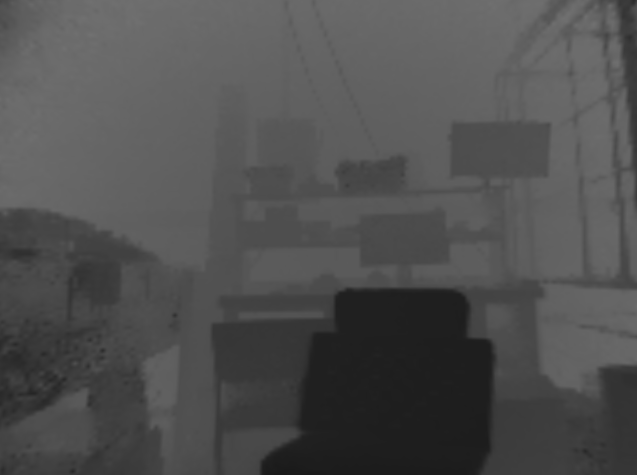
\includegraphics[width=4.8cm]{img/manip_0_0_1_a.png}
\end{subfigure}%
\begin{subfigure}{5cm}
  \centering
  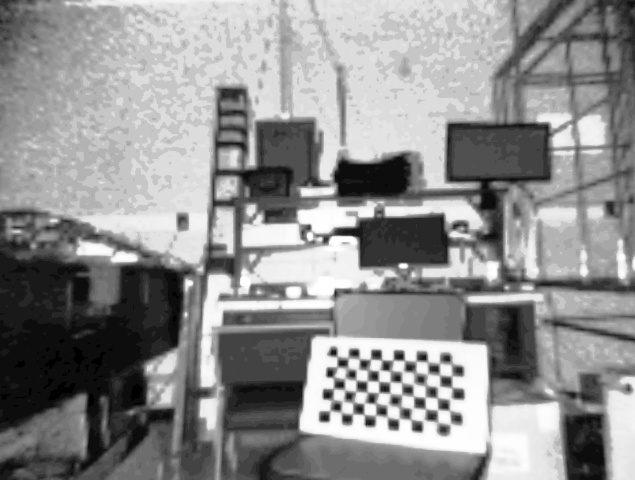
\includegraphics[width=4.8cm]{img/manip_0_0_1_b.png}
\end{subfigure}
\begin{subfigure}{5cm}
  \centering
  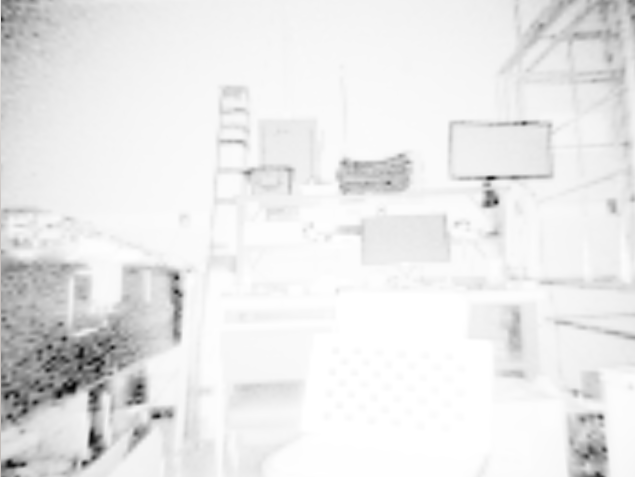
\includegraphics[width=4.8cm]{img/manip_0_0_1_c.png}
\end{subfigure}
\caption{Left: depth image - the darker, the nearer. Center: visual image. Right: confidence image - the variance is high on objects rims (scattering), on the picture edges (sensor limitations) and on some surfaces (thermal noise).}
\label{fig:manip_0_0_1}
\end{center}
\end{figure}
The limited range is highlighted in figure \ref{fig:manip_0_0_2} where an object is put a few centimeters away from the camera. The confidence becomes extremely bad (black) as the measured distance is clearly far from reality.
% figure manip_0_0_2
\begin{figure}[!htt]
\begin{center}
\begin{subfigure}{5cm}
  \centering
  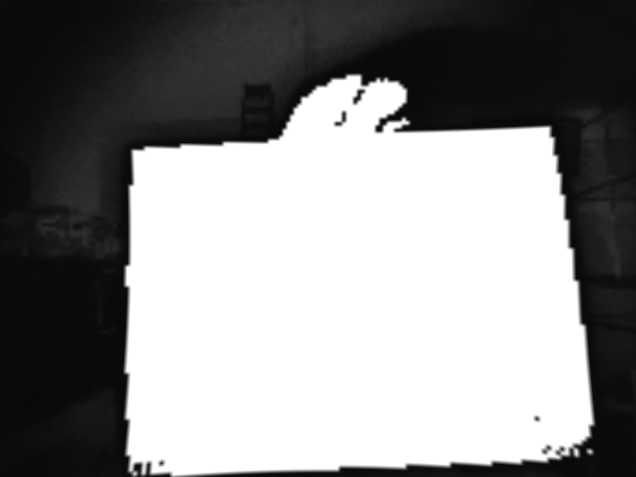
\includegraphics[width=4.8cm]{img/manip_0_0_2_a.png}
\end{subfigure}%
\begin{subfigure}{5cm}
  \centering
  
\includegraphics[width=4.8cm]{img/manip_0_0_2_b.png}
\end{subfigure}
\begin{subfigure}{5cm}
  \centering
  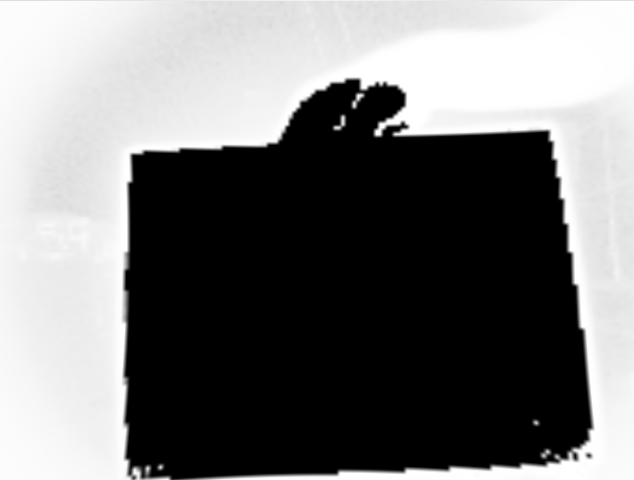
\includegraphics[width=4.8cm]{img/manip_0_0_2_c.png}
\end{subfigure}
\caption{When the object exceed the range limitation of the camera, the measurement can be twisted.}
\label{fig:manip_0_0_2}
\end{center}
\end{figure}
In figure \ref{fig:manip_0_0_3}, the same object is held a little farther so it can be measured correctly. However, the low luminosity induces the automatic exposure regulation to wait a little longer during the capture in order to make a good measurement, leading to very noisy pictures when the environment is brighter.
% figure manip_0_0_3
\begin{figure}[!htt]
\begin{center}
\begin{subfigure}{5cm}
  \centering
  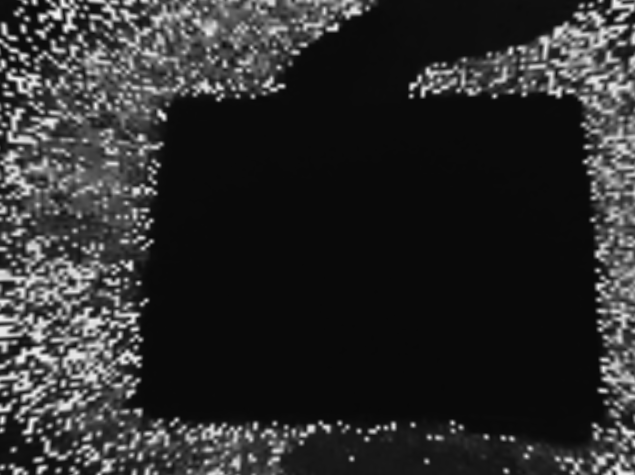
\includegraphics[width=4.8cm]{img/manip_0_0_3_a.png}
\end{subfigure}%
\begin{subfigure}{5cm}
  \centering
  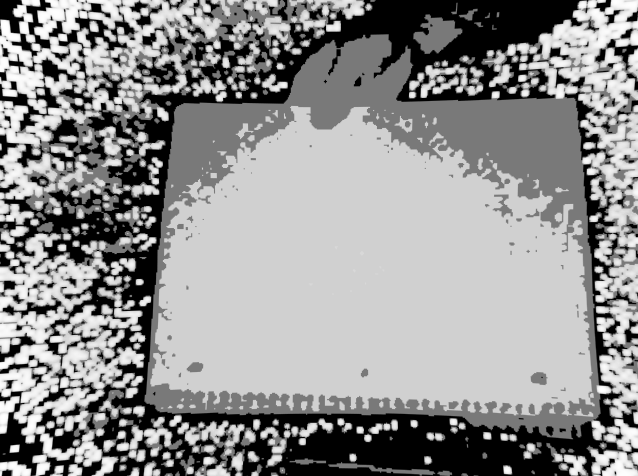
\includegraphics[width=4.8cm]{img/manip_0_0_3_b.png}
\end{subfigure}
\begin{subfigure}{5cm}
  \centering
  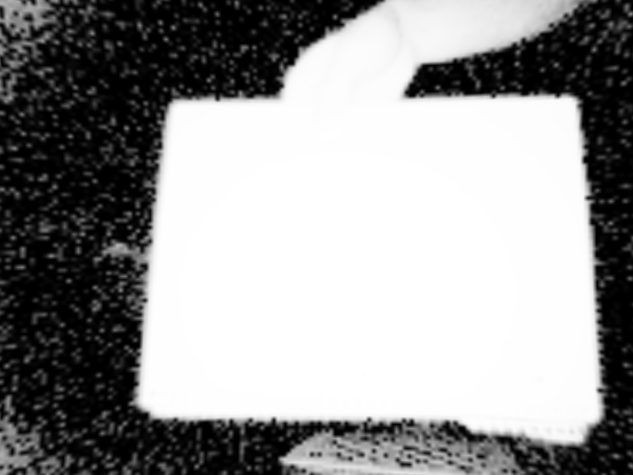
\includegraphics[width=4.8cm]{img/manip_0_0_3_c.png}
\end{subfigure}
\caption{If the object is too close (even if respecting the range limitation), auto-exposure can lead to very high noise in the background.}
\label{fig:manip_0_0_3}
\end{center}
\end{figure}
Figure \ref{fig:manip_0_0_4} illustrates that the quality of the measurement is material-dependent. Here, the reflection of an aluminum slab corrupts the depth and visual pictures when the computation of confidence does not highlight the problem everywhere on the slab which means that the quality of a measurement cannot be qualified by the confidence picture only.
% figure manip_0_0_4
\begin{figure}[!htt]
\begin{center}
\begin{subfigure}{5cm}
  \centering
  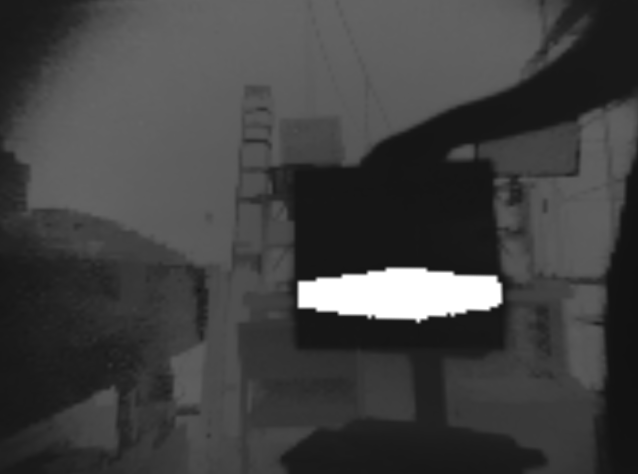
\includegraphics[width=4.8cm]{img/manip_0_0_4_a.png}
\end{subfigure}%
\begin{subfigure}{5cm}
  \centering
  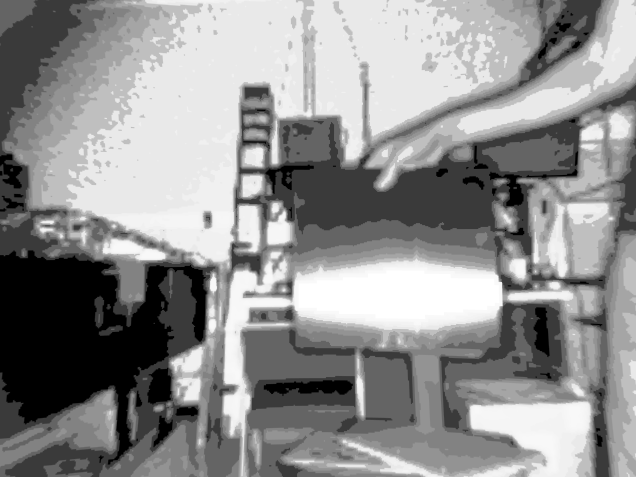
\includegraphics[width=4.8cm]{img/manip_0_0_4_b.png}
\end{subfigure}
\begin{subfigure}{5cm}
  \centering
  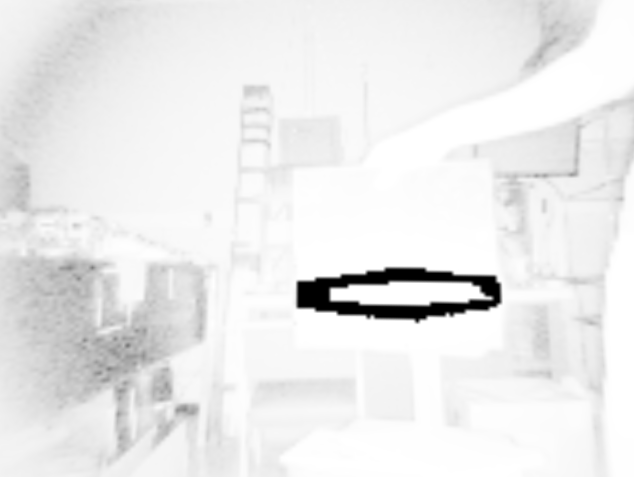
\includegraphics[width=4.8cm]{img/manip_0_0_4_c.png}
\end{subfigure}
\caption{The nature of the material (here some aluminum) changes the reflection properties, hence the measurement quality.}
\label{fig:manip_0_0_4}
\end{center}
\end{figure}
Last but not least, the problem of relative movement between the camera and the environment is presented in figure \ref{fig:manip_0_0_5}. On those pictures, a checkerboard is moved with a speed barely higher than a few centimeters per second and leads to very bad results. This can be a very important issue in space where the studied system is supposed to track and analyze the properties of spinning and tumbling targets.
% figure manip_0_0_5
\begin{figure}[!htt]
\begin{center}
\begin{subfigure}{5cm}
  \centering
  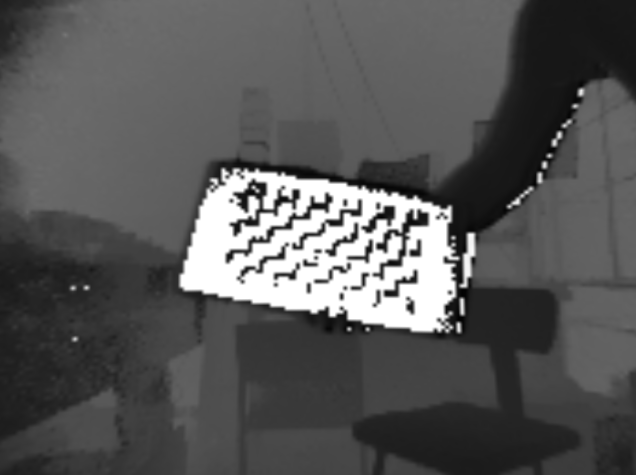
\includegraphics[width=4.8cm]{img/manip_0_0_5_a.png}
\end{subfigure}%
\begin{subfigure}{5cm}
  \centering
  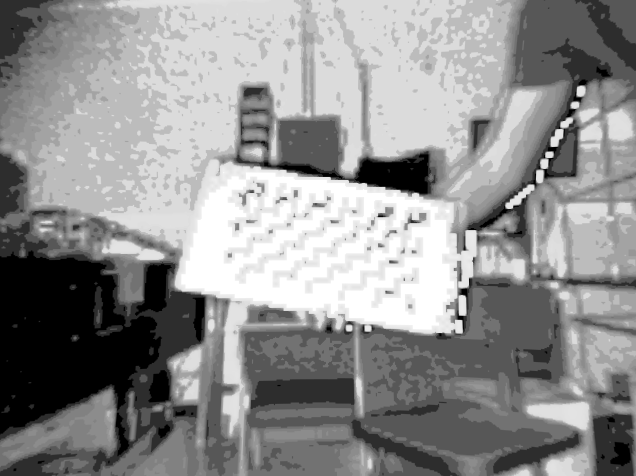
\includegraphics[width=4.8cm]{img/manip_0_0_5_b.png}
\end{subfigure}
\begin{subfigure}{5cm}
  \centering
  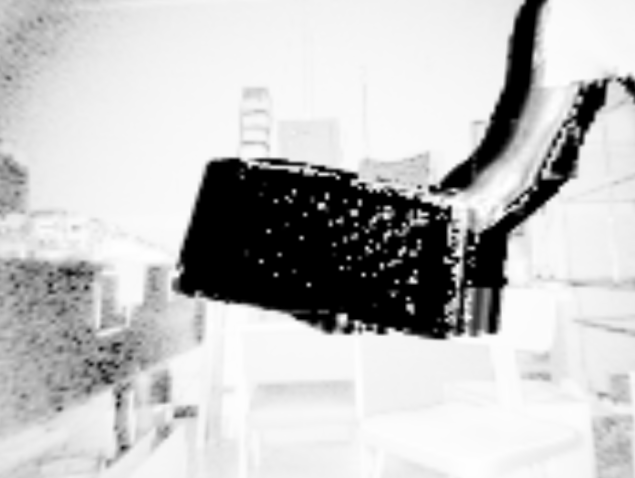
\includegraphics[width=4.8cm]{img/manip_0_0_5_c.png}
\end{subfigure}
\caption{The movement is a decisive factor driving the measurement accuracy. A relative speed of a few dozens of centimeters per second causes a substantial error in the checkerboard depth measurement.}
\label{fig:manip_0_0_5}
\end{center}
\end{figure}

\subsection{Calibration and distortions Rectification}
In figure \ref{fig:manip_0_1_1}, many typical pictures are taken in the limits of the space where checkerboards can be detected using only the visual image. From the coordinates of the points, the software gives the following \textit{intrinsic matrix}:
\begin{equation}
\begin{pmatrix}[0.8]
532.74 & 0 & 308.64\\
0 & 490.43 & 222.22\\
0 & 0 & 1
\end{pmatrix}
\end{equation}
Where the distances are in pixels. Given a pixel size of  $40 \mu m$ (see chapter \ref{chapter:intro}) and the picture scaling ratio of 3.68 along $U$ and 3.33 along $V$, we deduce $f_U = 5.9 mm$ and $f_V = 5.9 mm$ where the small differences with the values as provided by the constructor can be explained by a variable focal length. Besides, $c_U = 308$ and $c_V = 222$ are not far from the theoretical center $c_U = 320$ and $c_V = 240$. The distortion coefficients are equals to:
\begin{equation}
\label{eq:intrinsic}
\begin{pmatrix}[0.8]
-3.45e-01 & 1.44e-01 &-2.20e-04 & 1.91e-03 & 5.181e-02
\end{pmatrix}
\end{equation}
Figure \ref{fig:manip_0_1_2} shows the result after the distortion rectification for a very close object.

% Figure manip_0_1_1
\begin{figure}[!htt]
\begin{center}
\begin{subfigure}{5cm}
  \centering
  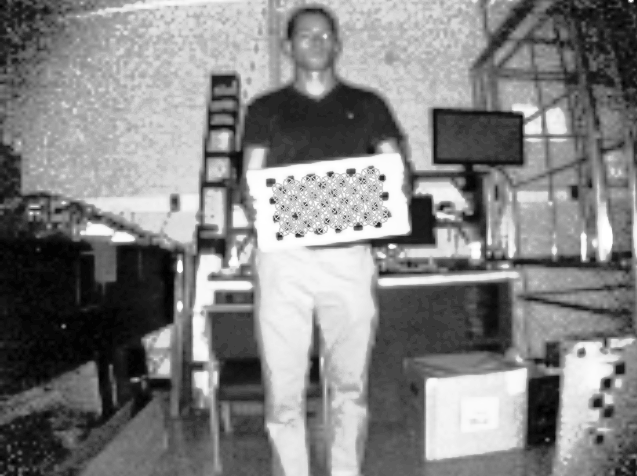
\includegraphics[width=4.8cm]{img/manip_0_1_1_a.png}
\end{subfigure}%
\begin{subfigure}{5cm}
  \centering
  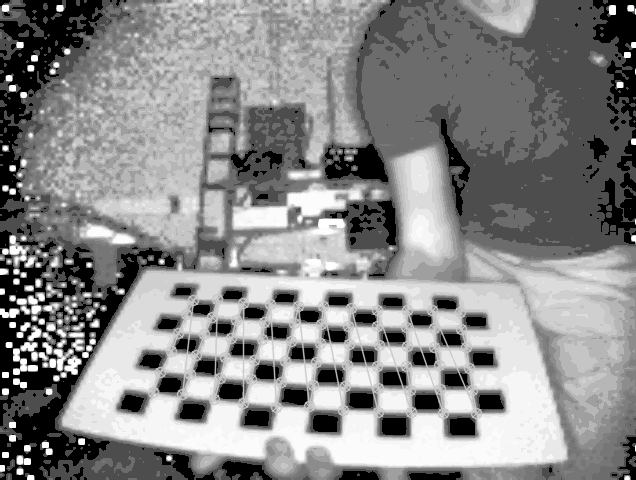
\includegraphics[width=4.8cm]{img/manip_0_1_1_b.png}
\end{subfigure}
\begin{subfigure}{5cm}
  \centering
  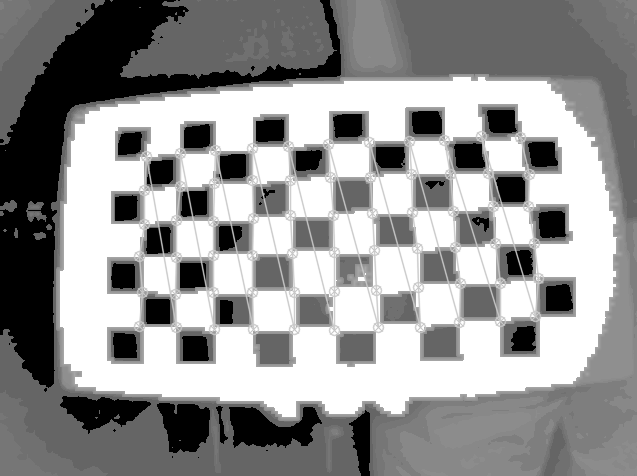
\includegraphics[width=4.8cm]{img/manip_0_1_1_c.png}
\end{subfigure}
\caption{We vary the checkerboard orientation to the limits of detection to cover the space at maximum. Left: the farthest distance. Center: the maximal inclination. Right: the closest distance.}
\label{fig:manip_0_1_1}
\end{center}
\end{figure}
% Figure manip_0_1_2
\begin{figure}[!htt]
\begin{center}
\begin{subfigure}{5cm}
  \centering
  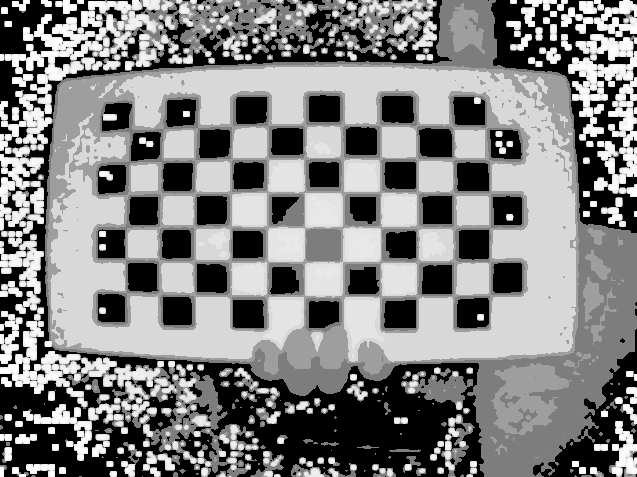
\includegraphics[width=4.8cm]{img/manip_0_1_2_a.png}
\end{subfigure}%
\begin{subfigure}{5cm}
  \centering
  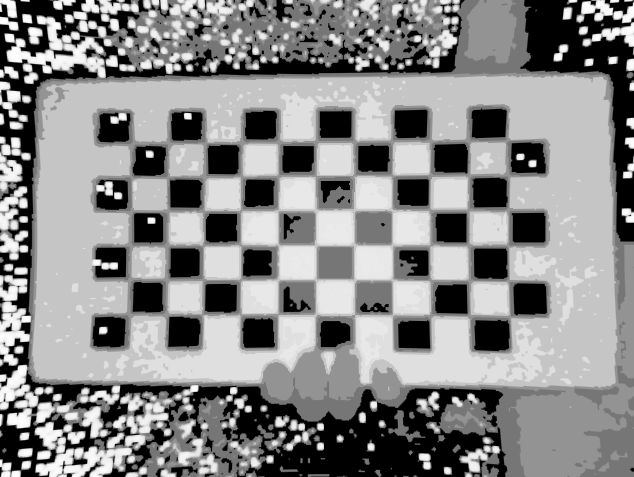
\includegraphics[width=4.8cm]{img/manip_0_1_2_b.png}
\end{subfigure}
\caption{Left: a checkerboard before rectification. Right: the same checkerboard after the distortions rectification. The edges are now straight and parallel.}
\label{fig:manip_0_1_2}
\end{center}
\end{figure}
\subsection{Absolute Depth Measurement}
In this paragraph, one of the examples implemented with this project software is used to compute the depth of a calibration target situated $1m$ away from the \gls{ORF} camera (figure \ref{fig:manip_0_2_1}). 
% Figure fig:manip_0_2_1
\begin{figure}[!htt]
\begin{center}
  \centering
  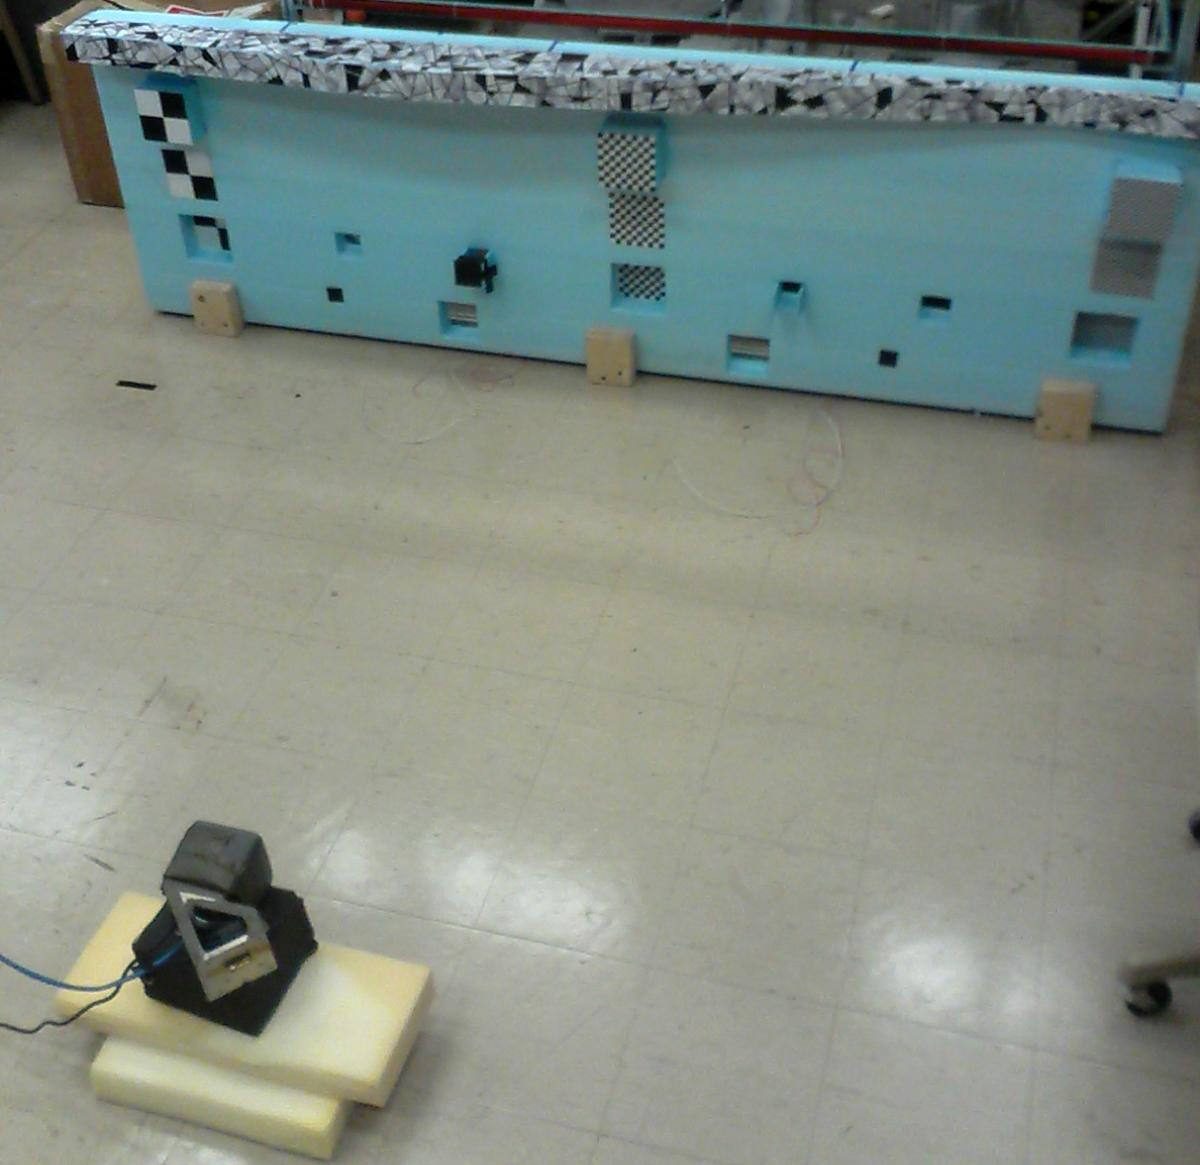
\includegraphics[width=7cm]{img/orf_meas_setup.jpg}
\caption{The setup used for \gls{ORF} calibration.}
\label{fig:manip_0_2_1}
\end{center}
\end{figure}
To take the noise into account, the capture of figure \ref{fig:manip_0_2_2} is realized several times to compensate the thermal noise of $1.026mm$. This difference of a few millimeters is explained by the inaccuracy of the setup itself, the material reflectivity, and the fact that the measured point is not directly along the focal axis (we then measure the hypothesis as presented in figure \ref{fig:orf_depth})
% Figure fig:manip_0_2_2
\begin{figure}[!htt]
\begin{center}
\begin{subfigure}{5cm}
  \centering
  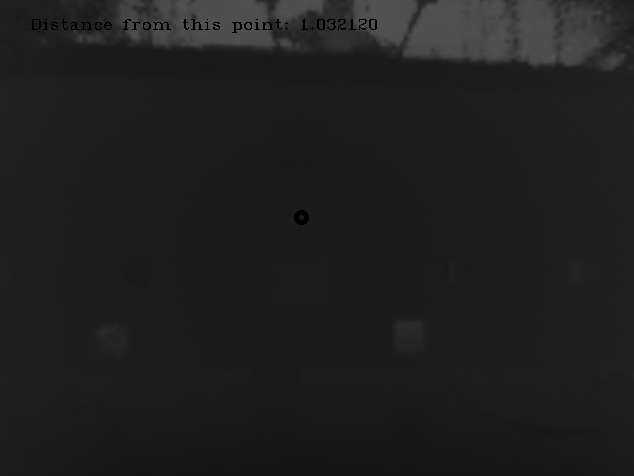
\includegraphics[width=4.8cm]{img/manip_0_2_2_a.png}
\end{subfigure}%
\begin{subfigure}{5cm}
  \centering
  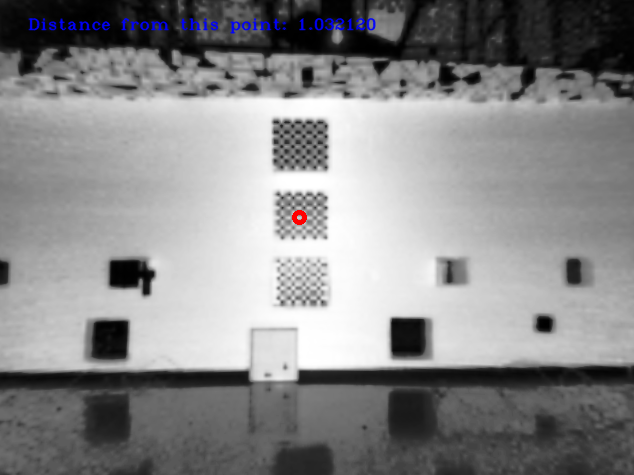
\includegraphics[width=4.8cm]{img/manip_0_2_2_b.png}
\end{subfigure}
\begin{subfigure}{5cm}
  \centering
  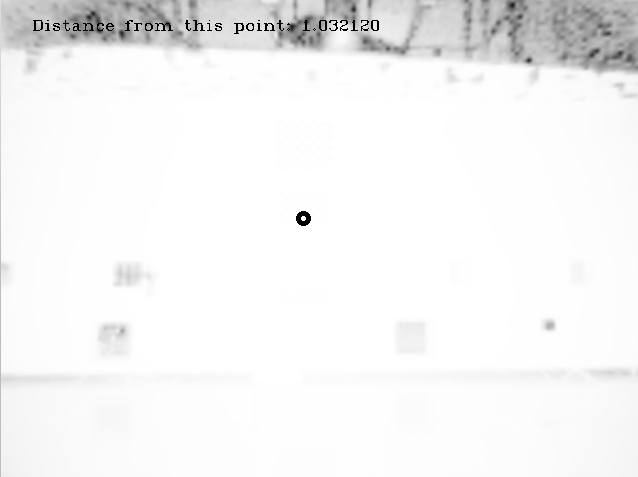
\includegraphics[width=4.8cm]{img/manip_0_2_2_c.png}
\end{subfigure}
\caption{Several measurement are effectuated in the center of the target and their mean is computed to compensate Gaussian noise.}
\label{fig:manip_0_2_2}
\end{center}
\end{figure}
This last effect is showed in figure \ref{fig:manip_0_2_3}, where the measured depth is equal to $1.159m$ when the $Z$ coordinate should be still about $1m$.
% Figure fig:manip_0_2_3
\begin{figure}[!htt]
\begin{center}
\begin{subfigure}{5cm}
  \centering
  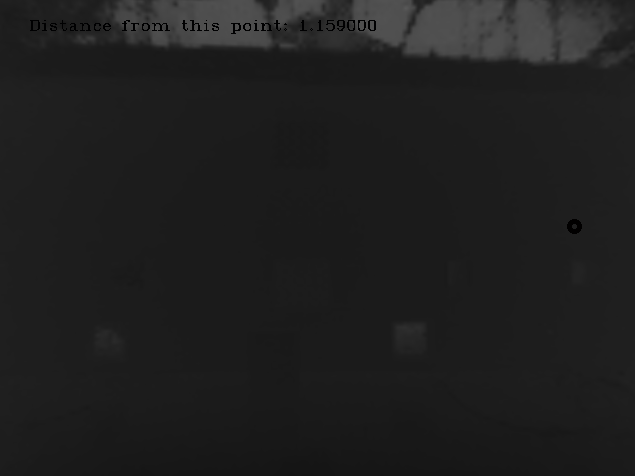
\includegraphics[width=4.8cm]{img/manip_0_2_3_a.png}
\end{subfigure}%
\begin{subfigure}{5cm}
  \centering
  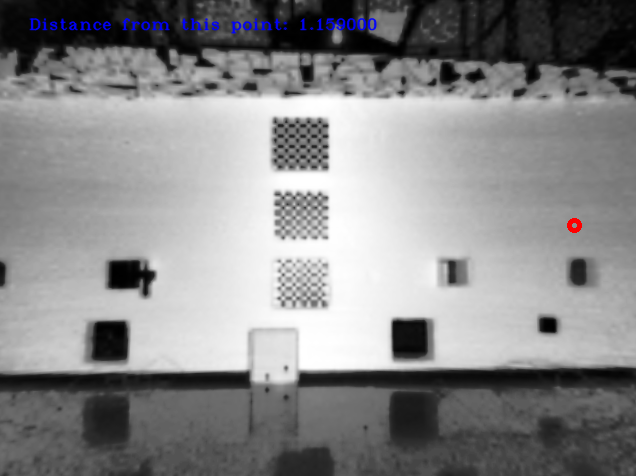
\includegraphics[width=4.8cm]{img/manip_0_2_3_b.png}
\end{subfigure}
\begin{subfigure}{5cm}
  \centering
  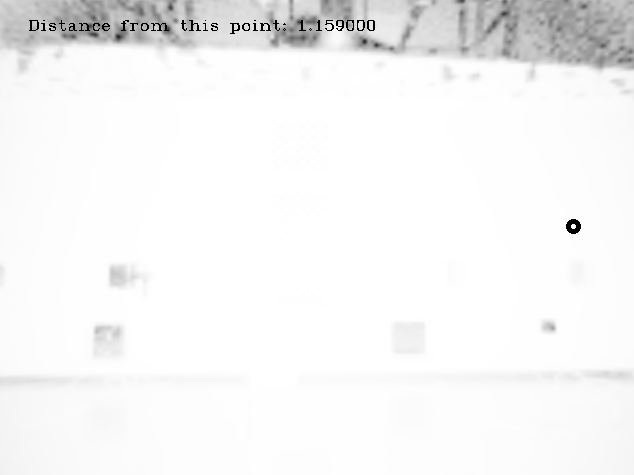
\includegraphics[width=4.8cm]{img/manip_0_2_3_c.png}
\end{subfigure}
\caption{The same measurement are made on the right of the target to illustrate the problem of $XYZ$ reconstruction from the depth.}
\label{fig:manip_0_2_3}
\end{center}
\end{figure}

\subsection{Relative Depth Measurement}
Using the data of the two last paragraphs, we can also compute $XYZ$ coordinates in the $T$ coordinate system using pinhole inversion. This time, we perform six captures in three targets presenting a relative difference of $2 inches$ in $Z$ coordinates and we compute this relative distance to get rid of the systemic error in the setup accuracy (figure \ref{fig:manip_0_3_1}). We obtain then:
%Figure manip_0_3_1
\begin{figure}[!htt]
\begin{center}
\begin{subfigure}{5cm}
  \centering
  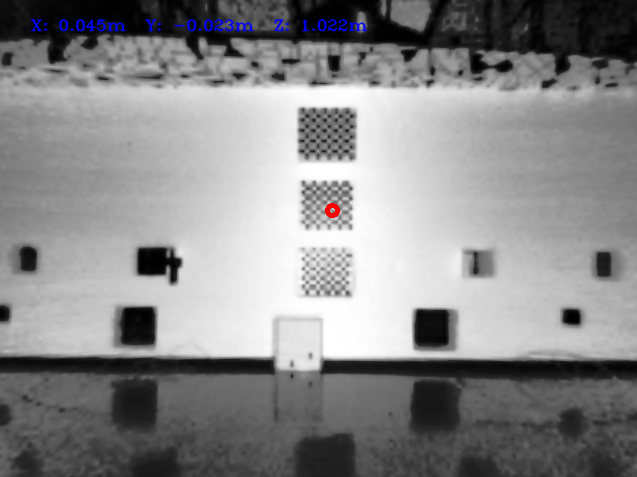
\includegraphics[width=4.8cm]{img/manip_0_3_1_a.png}
\end{subfigure}%
\begin{subfigure}{5cm}
  \centering
  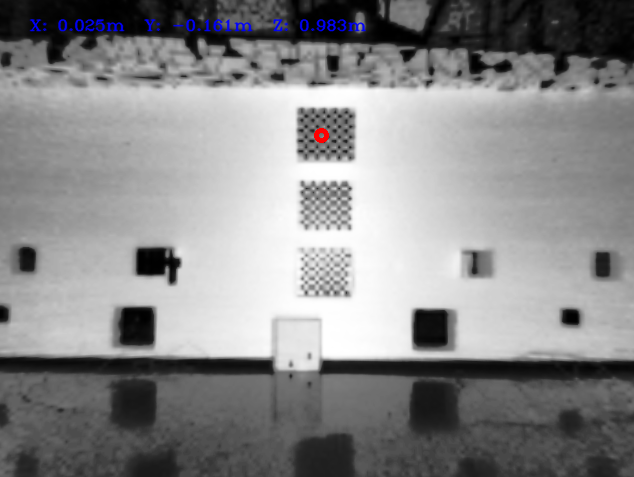
\includegraphics[width=4.8cm]{img/manip_0_3_1_b.png}
\end{subfigure}
\begin{subfigure}{5cm}
  \centering
  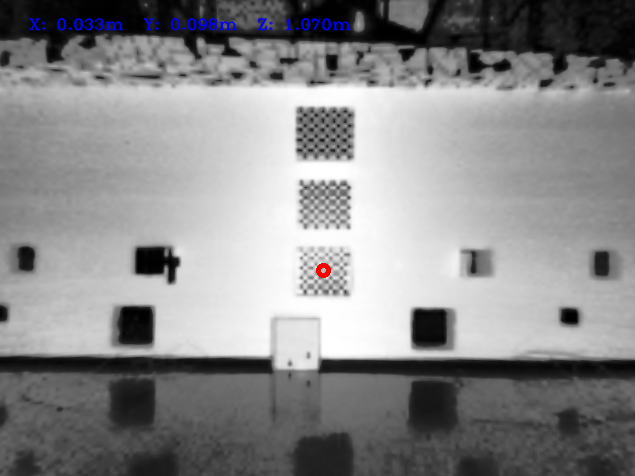
\includegraphics[width=4.8cm]{img/manip_0_3_1_c.png}
\end{subfigure}
\caption{The mean $XYZ$ coordinates are computed for three different points to deduce the relative $Z$ distance between them and compare it to the reference benchmark.}
\label{fig:manip_0_3_1}
\end{center}
\end{figure}
To be more general and verify that $X$ and $Y$ coordinates are also correct (they depends on $f_U$, $f_V$, $c_U$, $c_V$ unlike the $Z$ coordinate) we can also measure the euclidean distance between two vertexes of a target with a known geometry framed by a camera with a random angle and distance (figure \ref{fig:manip_0_3_2}). Once again, this experiment is repeated several times and the mean distance is computed:
\begin{equation}
\bar{d} = \sqrt{(\bar{x_1} - \bar{x_2})^2 + (\bar{y_1} - \bar{y_2})^2 + (\bar{z_1} - \bar{z_2})^2} = 6.24 cm
\end{equation}
Which is blaaaaaa compared to the blaaaaa we were supposed to obtain.
%Figure manip_0_3_2
\begin{figure}[!htt]
\begin{center}
\begin{subfigure}{5cm}
  \centering
  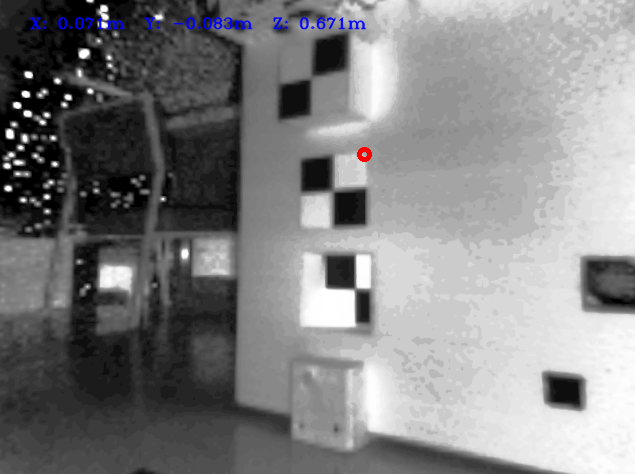
\includegraphics[width=4.8cm]{img/manip_0_3_2_a.png}
\end{subfigure}%
\begin{subfigure}{5cm}
  \centering
  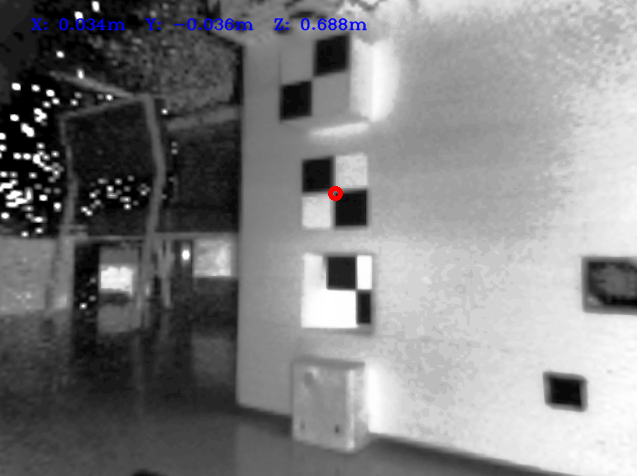
\includegraphics[width=4.8cm]{img/manip_0_3_2_b.png}
\end{subfigure}
\caption{The mean $XYZ$ coordinates are computed for two different points to deduce the euclidean distance between them and compare it to the reference benchmark.}
\label{fig:manip_0_3_2}
\end{center}
\end{figure}


\subsection{3D Points Cloud Construction}
\label{subsec:3D_reconstruction}
In these last experiments, a point cloud is constructed using the \gls{PCL} library tools included in the software developed in this project. In figure \ref{fig:manip_0_4_1}, two views of the same points cloud are given. We can notice that the visual image is included in the process since we can see the pattern on the checkerboard. The importance of the scattering and the thermal noise can be highlighted especially if we look precisely to the edges of the checkerboard and its shape from above (which is supposed to be flat).
%Figure manip_0_4_1
\begin{figure}[!htt]
\begin{center}
\begin{subfigure}{7cm}
  \centering
  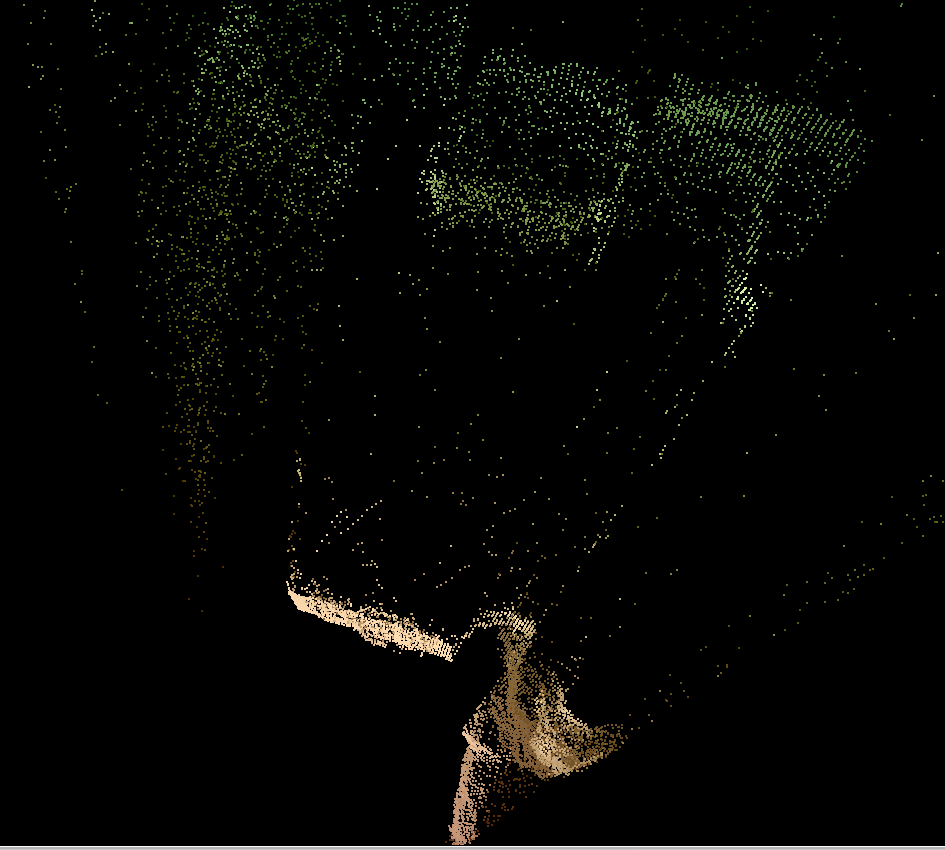
\includegraphics[width=6.8cm]{img/manip_0_4_1_a.png}
\end{subfigure}%
\begin{subfigure}{7cm}
  \centering
  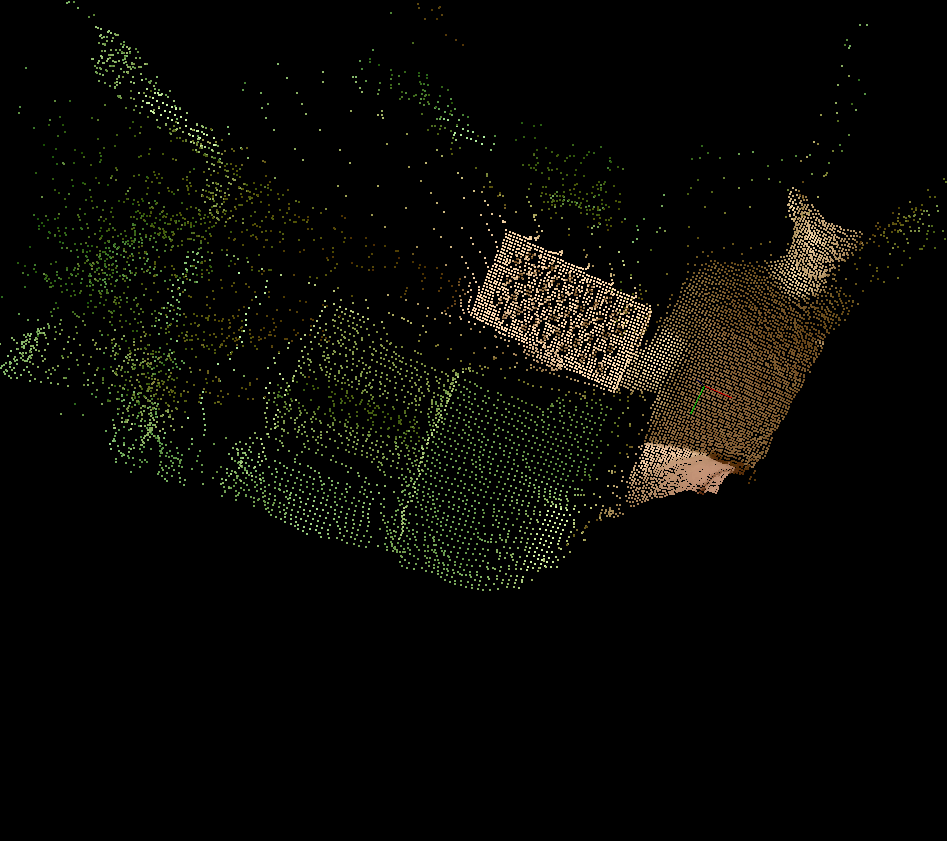
\includegraphics[width=6.8cm]{img/manip_0_4_1_b.png}
\end{subfigure}
\caption{A 3D points cloud with visual information reconstructed from \gls{ORF} pictures. Scattering around edges and thermal noise in the background can be observed.}
\label{fig:manip_0_4_1}
\end{center}
\end{figure}
Figure \ref{fig:manip_0_4_2} illustrates the importance of the noise due to auto-exposure when an object is very close to the lens.
%Figure manip_0_4_2
\begin{figure}[!htt]
\begin{center}
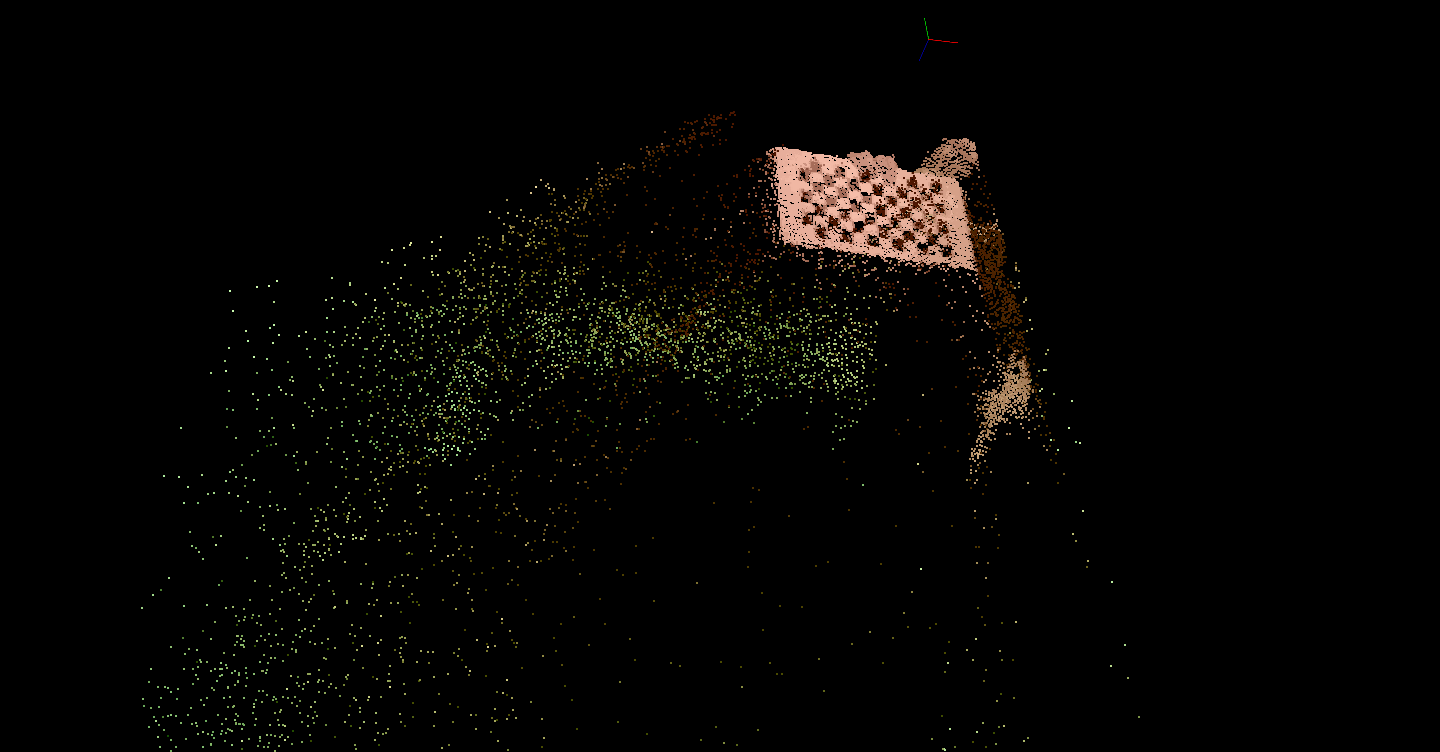
\includegraphics[width=10cm]{img/manip_0_4_2.png}
\caption{When the target is too close from the camera, the background becomes very noisy because of the auto-exposure.}
\label{fig:manip_0_4_2}
\end{center}
\end{figure}

\section{Stereo Acquisition}
In this section, we will discuss the efficiency of the VERTIGO sensors and algorithm. As a lot of work has already been done on the subject, for instance in \cite{vertigo_phd}, \cite{muggler_phd} and \cite{makowka_phd}, this project simply focused on the comparison with the \gls{ORF} camera and points out the complementarity of the two systems.

The reconstruction of a 3D points cloud from stereo sensors is performed through the elaboration of a disparity map, whose information is quite similar to that of the \gls{ORF} depth map. To create this disparity map, different techniques can be used, a taxonomy of those is given in \cite{stereo_methods_comparaison}. Basically, the process always implies the following steps: features detection and matching, aggregation, disparity computation and optimization. The quality of the disparity image is dependent on the number of matchable features, called supporting points, in the left and right pictures: if the considered environment is highly textured, this will lead to accurate 3D reconstruction while uniform patches will not give reliable results. The interstices between supporting points is filled by aggregation methods around those points which have also a lot of influence on the final disparity map. In figure \ref{fig:manip_1_1}, the results of a block matching stereo function provided in OpenCV libraries illustrate our remarks.
% Figure manip_1_1
\begin{figure}[!htt]
\begin{center}
\begin{subfigure}{5cm}
  \centering
  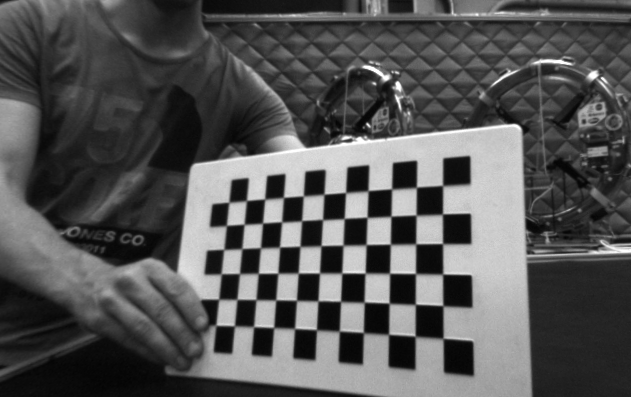
\includegraphics[width=4.8cm]{img/manip_1_1_a.png}
\end{subfigure}%
\begin{subfigure}{5cm}
  \centering
  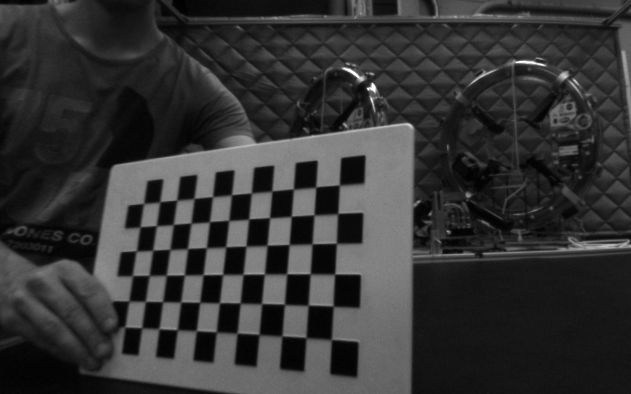
\includegraphics[width=4.8cm]{img/manip_1_1_b.png}
\end{subfigure}
\begin{subfigure}{4cm}
  \centering
  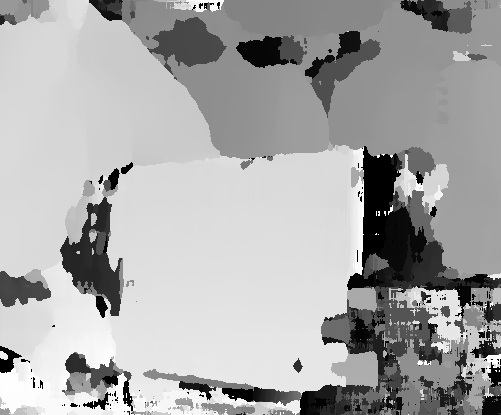
\includegraphics[width=3.8cm]{img/manip_1_1_c.png}
\end{subfigure}
\caption{Left: Left image. Center: Right image. Right: disparity map reconstructed with OpenCV stereo block matching function - the checkerboard (high textured) gives a good result when the patch in the bottom right corner (uniform) is badly represented.}
\label{fig:manip_1_1}
\end{center}
\end{figure}
However, if the stereo vision algorithms suffer from this texture dependency, they do not encounter the same problems as the \gls{ORF} in term of movement and luminosity conditions. This complementarity has been proved qualitatively with the use of a setup involving the \gls{ORF} and the VERTIGO goggles capturing simultaneous pictures of the same object. 
% Figure manip_1_2
\begin{figure}[!htt]
\begin{center}
\begin{subfigure}{4.2cm}
  \centering
  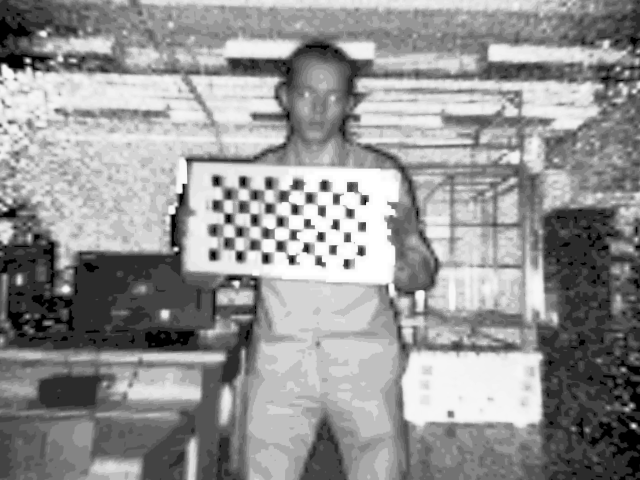
\includegraphics[width=3.8cm]{img/manip_1_2_a.png}
\end{subfigure}%
\begin{subfigure}{4cm}
  \centering
  \includegraphics[width=3.8cm]{img/manip_1_2_b.png}
\end{subfigure}
\begin{subfigure}{4cm}
  \centering
  \includegraphics[width=3.8cm]{img/manip_1_2_c.png}
\end{subfigure}
\vspace{0.5cm}
\begin{subfigure}{5cm}
  \centering
  \includegraphics[width=3.8cm]{img/manip_1_2_d.png}
\end{subfigure}%
\begin{subfigure}{4cm}
  \centering
  \includegraphics[width=3.8cm]{img/manip_1_2_e.png}
\end{subfigure}
\begin{subfigure}{4cm}
  \centering
  \includegraphics[width=3.8cm]{img/manip_1_2_f.png}
\end{subfigure}
\caption{Above: visual, confidence and depth images captured with the ORF - the movement induces a error in the depth measurement. Below: Left and right images of the stereo sensor and the disparity map - even with the movement, the result is acceptable for the checkerboard.}
\label{fig:manip_1_2}
\end{center}
\end{figure}
In figure \ref{fig:manip_1_2}, the movement reliability is highlighted: a checkerboard animated with a speed of the few dozen of centimeters per second is captured by the two sensors. Even if the stereo images could be considered a little more blurred than in the static case, they are still sufficient to detect features and a disparity map can be more reliable for textured pattern than the \gls{ORF} depth map.
% Figure manip_1_3
\begin{figure}[!htt]
\begin{center}
\begin{subfigure}{4.2cm}
  \centering
  \includegraphics[width=3.8cm]{img/manip_1_3_a.png}
\end{subfigure}%
\begin{subfigure}{4cm}
  \centering
  \includegraphics[width=3.8cm]{img/manip_1_3_b.png}
\end{subfigure}
\begin{subfigure}{4cm}
  \centering
  \includegraphics[width=3.8cm]{img/manip_1_3_c.png}
\end{subfigure}
\vspace{0.5cm}
\begin{subfigure}{4cm}
  \centering
  \includegraphics[width=3.8cm]{img/manip_1_3_d.png}
\end{subfigure}%
\begin{subfigure}{4cm}
  \centering
  \includegraphics[width=3.8cm]{img/manip_1_3_e.png}
\end{subfigure}
\begin{subfigure}{4cm}
  \centering
  \includegraphics[width=3.8cm]{img/manip_1_3_f.png}
\end{subfigure}
\caption{Above: visual, confidence and depth images captured with the ORF - as the checkerboard is too close, the depth measurement is very bad. Below: Left and right images of the stereo sensor and the disparity map - the checkerboard depth measurement is still correct near the camera.}
\label{fig:manip_1_3}
\end{center}
\end{figure}
An illustration of the range reliability is given in figure \ref{fig:manip_1_3} where the \gls{ORF} shows difficulty to estimate correctly the depth of a checkerboard too close to the camera when the stereo sensors will not notice any difference.


\section{Multi-sensors Calibration}
To determine the performances of the calibration algorithm we discussed in section \ref{subsec:system_calib}, we connect the \gls{ORF} and the stereo cameras to the VERTIGO computer and we acquire synchronous images of a checkerboard (figure \ref{fig:manip_2_1}). It is important for each capture to make sure the checkerboard is not moving and the luminous conditions are sufficient by checking the confidence picture (figure \ref{fig:manip_2_2}).

% Figure manip_2_1
\begin{figure}[!htt]
\begin{center}
\includegraphics[width=10cm]{img/manip_2_1.jpg}
\caption{The experiment setup: VERTIGO and the ORF camera fixed to the Halo and plugged to the embedded computer.}
\label{fig:manip_2_1}
\end{center}
\end{figure}
% Figure manip_2_2
\begin{figure}[!htt]
\begin{center}
\begin{subfigure}{3cm}
  \centering
  \includegraphics[width=2.8cm]{img/manip_2_2_a.png}
\end{subfigure}%
\begin{subfigure}{2.9cm}
  \centering
  \includegraphics[width=2.8cm]{img/manip_2_2_b.png}
\end{subfigure}
\begin{subfigure}{2.9cm}
  \centering
  \includegraphics[width=2.8cm]{img/manip_2_2_c.png}
\end{subfigure}
\begin{subfigure}{2.9cm}
  \centering
  \includegraphics[width=2.8cm]{img/manip_2_2_d.png}
\end{subfigure}
\begin{subfigure}{2.9cm}
  \centering
  \includegraphics[width=2.8cm]{img/manip_2_2_e.png}
\end{subfigure}
\vspace{0.5cm}
\begin{subfigure}{3cm}
  \centering
  \includegraphics[width=2.8cm]{img/manip_2_2_f.png}
\end{subfigure}%
\begin{subfigure}{2.9cm}
  \centering
  \includegraphics[width=2.8cm]{img/manip_2_2_g.png}
\end{subfigure}
\begin{subfigure}{2.9cm}
  \centering
  \includegraphics[width=2.8cm]{img/manip_2_2_h.png}
\end{subfigure}
\begin{subfigure}{2.9cm}
  \centering
  \includegraphics[width=2.8cm]{img/manip_2_2_i.png}
\end{subfigure}
\begin{subfigure}{2.9cm}
  \centering
  \includegraphics[width=2.8cm]{img/manip_2_2_j.png}
\end{subfigure}
\caption{Above: a bad capture for calibration (from left to right: left image, right image, depth image, confidence image, ORF visual image). Below: a good capture (same meaning).}
\label{fig:manip_2_2}
\end{center}
\end{figure}
We then proceed to corner detection in those images and reconstruct separately the 3D corresponding points for the \gls{ORF} (in the $T$ coordinate system) and the stereo cameras (in the $L$ coordinate system). The transformation matrix between them being still unknown, those points are represented in the same 3D visualization assuming a common origin (figure \ref{fig:manip_2_3}). 
% Figure manip_2_3
\begin{figure}[!htt]
\begin{center}
\includegraphics[width=14cm]{img/manip_2_3.png}
\caption{ORF and stereo reconstructed checkerboard are represented on the same image. Dark blue: stereo board 1. Light blue: ORF board 1. Red: stereo board 2. Rose: ORF board 2. Yellow: stereo board 3. Orange: ORF board 3. Dark green: stereo board 4. Light green: ORF board 4. Dark violet: stereo board 5. Light violet: ORF board 5.}
\label{fig:manip_2_3}
\end{center}
\end{figure}
It is important to understand though that this has no physical meaning, it is just a way to verify a few parameters like the size of the cloud, the regularity of the checkerboard, their straightness or the noise. For example, we can notice the noise more important with the \gls{ORF} as predicted theoretically (figure \ref{fig:manip_2_4}). The RANSAC scheme will help to put aside the points that are too distant each other. The points evaluated by the stereo sensors are more accurate, since the triangulation process is based on feature matching, which is an easier problem for checkerboard corner detection. Hence, the accuracy is driven by the theoretical definition of equation \ref{eq:stereo_acc}, though the focal length and the baseline values depend on the stereo calibration efficiency.


% Figure manip_2_4
\begin{figure}[!htt]
\begin{center}
\begin{subfigure}{7cm}
  \centering
  \includegraphics[width=6.8cm]{img/manip_2_4_a.png}
\end{subfigure}%
\begin{subfigure}{7cm}
  \centering
  \includegraphics[width=6.8cm]{img/manip_2_4_b.png}
\end{subfigure}
\caption{Left: the ORF reconstructed checkerboard (light blue) is noisier than the stereo one (dark blue) in the $Z$ direction. Right: this effect is less pronounced in the $XY$ plane. The holes are due to rejection of the points considered as too noisy.}
\label{fig:manip_2_4}
\end{center}
\end{figure}
A way to check the reliability of the 3D reconstruction is to compute the euclidean distances between each point and compare them to the theoretical $25mm$ of the real checkerboard. On the whole, those distances are always situated around $30mm$ and are bigger for \gls{ORF} which makes theoretical sense, since the noise, naturally higher for the ORF, always has a positive contribution on distance measurements.

In the next part of the process, the sum of the distances between the range finder and the stereo device is minimized and extrinsic matrices are computed. Here, we display the $M_{TL}$ matrices of a calibration using 7 checkerboard capture with the sensors plugged on the Halo.\\
With RANSAC:
\begin{equation}
\begin{pmatrix}[0.7]
0.998 & 0.0465 & 0.0294 & -0.166\\
-0.0456 & 0.999 & -0.0299 & 0.00767\\
-0.0308 & 0.0285 & 0.999 & -0.0589\\
0 & 0 & 0 & 1
\end{pmatrix}
\end{equation}
Without RANSAC:
\begin{equation}
\begin{pmatrix}[0.7]
0.991 & 0.128 & -0.0435 & -0.14\\
-0.128 & 0.992 & -0.00107 & -0.00672\\
0.043 & 0.00663 & 0.999 & -0.0846\\
0 & 0 & 0 & 1
\end{pmatrix}
\end{equation}\\

In those matrices, we can see that the sensors are pretty aligned (rotation coefficient almost equal to 1 on the diagonal and 0 elsewhere) and we can compare the translations with the theoretical one measured on the CAD model of the \gls{INSPECT} project:
\begin{table}[H]
\begin{center}
\footnotesize
\begin{tabular}{|l|c|c|c|c|}
\hline
 & \multicolumn{2}{c|}{\textbf{CAD Model}} & \multicolumn{2}{c|}{\textbf{Calibration Results}}\\
 \hline
 & in \textit{inches} & in $cm$ & with RANSAC (in $cm$) & without RANSAC (in $cm$)\\
\hline
$X$ & 6.3345 & \textbf{16.09} & \textbf{16.6} & 14\\
\hline
$Y$ & 0.7903 & \textbf{2.01} & \textbf{0.77} & -0.67\\
\hline
$Z$ & 1.8662 & \textbf{4.74} & \textbf{5.89} & 8.46\\
\hline
\end{tabular}
\end{center}
\caption{Comparison of the theoretical and calibration results of the translation between the ORF and the left camera.}\label{table:calib}
\end{table}
Given the quality of the sensors and the global mechanical accuracy of the setup, we can consider those results to be quite good. However, it may be important to discuss the limitations:
\begin{itemize*}
\item \textbf{Stereo calibration parameters dependency}: First, as we just reminded, the stereo precision is a function of the focal length $f$ and the baseline $b$ between left and right cameras. Yet, those values are extracted from the stereo calibration and small imprecision on those can strongly affect the error on the final Halo calibration. Indeed, during the triangulation, errors on $b$ and $f$ will cause the reconstructed points cloud to inflate or deflate (figure \ref{fig:manip_2_5}). As the minimization process of this calibration calculates the rotation and translation between the geometric center of each cloud, the calibration will be then dependent on the localization of observed checkerboards (directly influencing the position of the cloud's geometric centers). A checkerboard situated essentially along the $X$ axis would lead to a higher error on $X$. In our example, we observe mainly checkerboard along $Z$ but one of them is shifted on the $Y$ axis, which explain the higher error on $Y$. It is important to understand that this problem is only due to the stereo imprecision, though. Because of this effect, the global observation drawn from all the calibration tests shows a bigger error in $Z$. As a matter of fact, if the checkerboards photographed during the calibration process are near the center of the $XY$ plane, they by necessity have a positive $Z$ coordinate.
\item \textbf{ORF noise}: Secondly, the noise of the \gls{ORF} is directed along the depth axis and is a function of the luminosity and the materials in the environment. Once again, as the cameras look at checkerboard with a positive $Z$, this component is more concerned by the calibration errors. However, the random nature of this process leads to an error with a zero mean value and then have a lower influence than the previous effect.
\end{itemize*}
% Figure manip_2_5
\begin{figure}[!htt]
\begin{center}
\includegraphics[width=12cm]{img/manip_2_5.png}
\caption{The ORF and stereo reconstructed checkerboard are now superposed thanks to the computed transformation matrix. If we look closely, the ORF checkerboard near the camera is shifted toward the camera when the farthest ORF checkerboard is shifted in the other direction. This highlights the fact that the stereo points cloud is too small, due to stereo calibration parameters inaccuracies.}
\label{fig:manip_2_5}
\end{center}
\end{figure}

\section{Multi-Sensor Fusion}
\subsection{Ground Results}
In this section, the results provided by images captured in the ground laboratory are analyzed. We use the setup in figure \ref{fig:manip_2_1} to acquire simultaneous pictures from the \gls{ORF} and \gls{VERTIGO} (figure \ref{fig:manip_3_1}).
% Figure manip_3_1
\begin{figure}[!htt]
\begin{center}
\begin{subfigure}{2.9cm}
  \centering
  \includegraphics[width=2.8cm]{img/manip_3_1_a.png}
\end{subfigure}
\begin{subfigure}{2.9cm}
  \centering
  \includegraphics[width=2.8cm]{img/manip_3_1_b.png}
\end{subfigure}
\begin{subfigure}{2.9cm}
  \centering
  \includegraphics[width=2.8cm]{img/manip_3_1_c.png}
\end{subfigure}%
\begin{subfigure}{2.9cm}
  \centering
  \includegraphics[width=2.8cm]{img/manip_3_1_d.png}
\end{subfigure}
\begin{subfigure}{2.9cm}
  \centering
  \includegraphics[width=2.8cm]{img/manip_3_1_e.png}
\end{subfigure}
\caption{A typical sample of input pictures for fusion. From left to right: ORF depth, ORF visual, ORF confidence, left image, right image.}
\label{fig:manip_3_1}
\end{center}
\end{figure}

With the data provided by the range finder, a 3D points cloud is built as in section \ref{subsec:3D_reconstruction} (figure \ref{fig:manip_3_5}). To gain in clearness, the 3D cloud is sub-sampled, though it would have been possible to do the same with each object in the \gls{FoV} of the three cameras without sub-sampling. The next step consists of computing the variance $\sigma_w^i$ of the \gls{ORF} total noise (thermal and scattering) assigned to each 3D point by using its depth map and the confidence map. Once this variance is computed, we can represent the interval $[d_T^i-3\sigma_w^i;\,d_T^i+3\sigma_w^i]$ around each point in the direction of the depth, defined by the axis linking this point and the optical center of the \gls{ORF}. This interval is discretized into steps whose width is equal to one quarter of the stereoscopic precision (figure \ref{fig:manip_3_5}).
% Figure manip_3_3
\begin{figure}[!htt]
\begin{center}
\begin{subfigure}{7cm}
  \centering
  \includegraphics[width=6.6cm]{img/manip_3_3_a.png}
\end{subfigure}
\begin{subfigure}{7.4cm}
  \centering
  \includegraphics[width=7.2cm]{img/manip_3_3_b.png}
\end{subfigure}
\caption{Left: in blue, the 3D ORF points; in green, a interval has been constructed around those points in function of the noise. Right: in blue and green, idem; in red, the 3D points computed in the end of the fusion.}
\label{fig:manip_3_3}
\end{center}
\end{figure}
Then, the coordinates of those points $p_T^{i,j}$ are moved in the left camera coordinate system $L$, and their projection on the left and right image planes of the stereo sensor is computed (figures \ref{fig:manip_3_3} and \ref{fig:manip_3_4}).
% Figure manip_3_4
\begin{figure}[!htt]
\begin{center}
\begin{subfigure}{7cm}
  \centering
  \includegraphics[width=6.8cm]{img/manip_3_4_a.png}
\end{subfigure}
\begin{subfigure}{7cm}
  \centering
  \includegraphics[width=6.8cm]{img/manip_3_4_b.png}
\end{subfigure}
\caption{The interval around each 3D point are reprojected in the stereo images (sub-sampled in the picture).}
\label{fig:manip_3_4}
\end{center}
\end{figure}
It is therefore possible to calculate the a-priori probability for the \gls{ORF} ($P[p^{i,j}|I_T]$) and the stereoscopic system ($P[p^{i,j}|I_L, I_R]$) and the joint probability ($P[p^{i,j}|I_T, I_L, I_R]$) which is minimized to find the new point $\hat{p}^i$ arising from the fusion (figure \ref{fig:manip_3_5}).
% Figure manip_3_5
\begin{figure}[!htt]
\begin{center}
\begin{subfigure}{7cm}
  \centering
  \includegraphics[width=6.6cm]{img/manip_3_5_a.png}
\end{subfigure}
\begin{subfigure}{7.2cm}
  \centering
  \includegraphics[width=7cm]{img/manip_3_5_b.png}
\end{subfigure}
\caption{Left: a flat checkerboard before fusion. Right: the same checkerboard after the fusion. Unlike the first theoretical assumptions, the fusion algorithm produces noise.}
\label{fig:manip_3_5}
\end{center}
\end{figure}
If we compare the results before and after the fusion, we can see that not only is the computation time at best ten times higher than the acquisition on a laptop computer, but the accuracy is worse after the fusion. We will discuss the reason further in this document.

\subsection{RGA Results}
As for the ground pictures, the fusion algorithm has been tested in a zero gravity environment provided by the NASA \gls{RGA}. To better understand the intent of this experiment, it may be important to remind the context of the project. Indeed, as mentioned in the introduction, this fusion algorithm is part of a \gls{SLAM} algorithm aiming at localizing, mapping and understanding the motion parameters of the objects around. Moreover, this algorithm is intended to be part of a control process meant for operation in an environment that cannot be reproduced outside a zero gravity environment. Tests in a  parabolic flights are then important to prove the reliability of the sensor fusion and acquisition as part as a full system as well as its performances in front of 6 \gls{DoF} moving objects. However, given the limited performances of the algorithm on the ground, this goal is difficult to achieve. We will then just focus on the complementarity of the \gls{VERTIGO} and \gls{ORF} by performing fusion on a set of pictures captured synchronously during \gls{RGA} flights.

TODO + Themrocam


\subsection{Discussion}
In this section, we showed that, despite the demonstrated complementary operation of \gls{VERTIGO} and the \gls{ORF}, the new fusion algorithm does not take full advantage of this complementarity. To discuss the explanations, we classified them into four categories.

\subsubsection{ORF default can induce fusion failure}
If this algorithm is supposed to enhance the accuracy of 3D cloud built with the \gls{ORF} measurements, the image capture makes it impossible for the stereo system to recover from bad images obtained by by the \gls{ORF}. This has been mainly observed during \gls{RGA} tests sessions in which saturation, significant relative speeds, and a too short range have provided inferior results whilst \gls{VERTIGO} alone could have done better. Using the notations of section \ref{subsec:fusion:overview}, we can say that \textbf{certainty} is not assured to increase with the fusion.

\subsubsection{Limited range}
As the size of the merged points cloud is defined by the subspace where all camera \gls{FoV} are crossing, this subspace is then smaller than \gls{VERTIGO} or the \gls{ORF} alone (hardware issue). In other words, the \textbf{completeness} decreases during the fusion process.

\subsubsection{Non-linearity of the stereo process}
The most important phenomenon that seems to explain the bad results of the algorithm is the following: to calculate the stereo probability, we use the projected points in the left and right image by associating a \textit{likeliness coefficient} to each couple of points (assuming a rectangular window around). However, it is notable in figure \ref{fig:manip_3_4} that small calibration errors lead to small shifts between left and right images (in other words, the projection does not point exactly the same detail as it should). When we build a 3D map from stereo pairs in a traditional way, we first match features then project them, which will cause small imprecisions we can deal with; the error can be linearized in this way. On the other hand, in the fusion algorithm case, we perform feature matching after the projection. Therefore, the matching can diverge in case of small calibration offsets; the error cannot be linearized in that way (figure \ref{fig:error}). In conclusion, those calibration errors makes the stereo probability to corrupt the final result: there is a loss in \textbf{accuracy}.
\begin{figure}[!htt]
\begin{center}
\begin{subfigure}{7.2cm}
  \centering
  \includegraphics[width=7cm]{img/fusion_error_1.png}
\end{subfigure}
\begin{subfigure}{7.2cm}
  \centering
  \includegraphics[width=7cm]{img/fusion_error_2.png}
\end{subfigure}
\caption{When the calibration error has a proportional impact on the result in the standard stereo 3D construction, this is not true in our algorithm.}
\label{fig:error}
\end{center}
\end{figure}

\section{Future Work}

\subsection{Improving Calibration}
As we concluded previously, the Halo calibration method that has been designed in this thesis looks promising. Ameliorations that could be implemented in the future are:
\begin{itemize*}
\item Improving the triangulation: if a simple method of triangulation is sufficient to process data in live, calibration must be very accurate at the expense of computation time. Many problems were discovered throughout the project due to the lack of calibration parameter accuracy.
\item Integrate the thermocam: to perform thermocam calibration, we can rely on the same methods as developed in the current version of the software. Intrinsic calibration could use the same OpenCV functions but a IR calibration pattern would be needed \cite{thermo_calib}, \cite{thermo_calib_2}. Concerning the extrinsic calibration, with the same pattern, a solution would be to integrate it into the stereo calibration and use a N-camera OpenCV function instead of the classical stereo calibration function.
\end{itemize*}

\subsection{Improving this Fusion Algorithm}
Despite the observed lack of robustness of the algorithm, it is possible to improve performance through:
\begin{itemize*}
\item Find a better function expressing the link between the confidence image and the thermal noise variance.
\item Minimize the error during the computation of the stereo probability by the use of a more reliable definition of the matches between stereo points despite of the calibration uncertainty.
\item At the end of the algorithm, build a thermal 3D point cloud by re-projecting the 3D point cloud in the thermocam image plane, read the value and combine it with the point position.
\end{itemize*}

\subsection{Building a New Fusion Algorithm}
Even if the issue concerning the stereo probability computation is overcome, there is still the problem of the lack of certainty: it requires good images from the \gls{ORF} as an input which seems not to be always true. Several tracks can be therefore explored:
\begin{itemize*}
\item \textbf{Keep a single stream}: the idea would be then to perform stereo triangulation first and improve it with the help of the ORF which does not require any matching function. However, the theoretical accuracy of the \gls{ORF} is supposed to be less and, once again, in case of bad images from stereo cameras (not enough textures), the entire process would suffer.
\item \textbf{Time division}: However, this would result in a fusion from a spatial point of view only and this does not correspond to the goals of the \gls{INSPECT} project.
\item \textbf{Spatial division}: The idea is to reconstruct two parallel 3D clouds with VERTIGO and the ORF in two different streams then use confidence and range to split the space into different parts. This time, the fusion is only temporal, which is also not the topic of the project.
\item \textbf{Other methods}: Quantity of promising methods are classified in \cite{stereo_tof_taxonomy}. When moving forward in the \gls{INSPECT} project, refinements could be done to select the most interesting.
\end{itemize*}

% % Fifth Chapter : Conclusions
%
% Master Thesis: Calibration and fusion of stereo cameras and optical-range finder sensors
% for in-space localization and mapping
%
% Achieved at Space System Lab, M.I.T.
% Supervisor: Alvar Saenz-Otero, Daniel Alazard
%
% Institut Sup�rieur de l'A�ronautique et de l'Espace
% Major: Telecommunications et r�seaux - Syst�mes Spatiaux et Lanceurs
% Gabriel Urbain - October 2014
%%

\chapter{Conclusions}
%\appendix
%\chapter{Tables}

\begin{table}
\caption{Armadillos}
\label{arm:table}
\begin{center}
\begin{tabular}{||l|l||}\hline
Armadillos & are \\\hline
our	   & friends \\\hline
\end{tabular}
\end{center}
\end{table}

\clearpage
\newpage

%\chapter{Figures}

\vspace*{-3in}

\begin{figure}
\vspace{2.4in}
\caption{Armadillo slaying lawyer.}
\label{arm:fig1}
\end{figure}
\clearpage
\newpage

\begin{figure}
\vspace{2.4in}
\caption{Armadillo eradicating national debt.}
\label{arm:fig2}
\end{figure}
\clearpage
\newpage

%% This defines the bibliography file (main.bib) and the bibliography style.
%% If you want to create a bibliography file by hand, change the contents of
%% this file to a `thebibliography' environment.  For more information 
%% see section 4.3 of the LaTeX manual.
\begin{singlespace}
\bibliography{main}
\bibliographystyle{plain}
\end{singlespace}

\end{document}

